\documentclass[10pt, a4paper, landscape]{article}

% -------------------------------------------------
% 宏包引入
% -------------------------------------------------
\usepackage[fontset=mac]{ctex}       % 中文支持
\usepackage{multicol}   % 多分栏
\usepackage{calc}
\usepackage{ifthen}
\usepackage{array}
\usepackage[landscape]{geometry} % 页面设置
\usepackage{amsmath,amsthm,amsfonts,amssymb} % 数学公式
\usepackage{color,graphicx,overpic} % 颜色与图片
\usepackage{hyperref}   % 超链接
\usepackage{enumitem}   % 列表环境控制
\usepackage{titlesec}   % 标题控制
\usepackage{bm}         % 加粗数学符号
\usepackage{xcolor}
\usepackage{tikz}       % 绘图


\usetikzlibrary{decorations.pathreplacing, positioning} % 加载brace装饰库
\usetikzlibrary{calc, positioning, arrows.meta, decorations.markings}
\setCJKmainfont{PingFang SC}
\setCJKsansfont{PingFang SC}
\setCJKmonofont{PingFang SC}

% -------------------------------------------------
% 自定义颜色
% -------------------------------------------------

\definecolor{myblue}{HTML}{003153} % 蓝色字
\definecolor{myred}{HTML}{85120F}  % 红色字
\definecolor{mygreen}{HTML}{218254}  % 绿色字
\definecolor{hlblue}{HTML}{ADC1DB} % 蓝色高亮
\definecolor{hlred}{HTML}{D66A83}  % 红色高亮
\definecolor{hlyellow}{HTML}{E3C79F}  % 奢金高亮
\definecolor{hlgreen}{HTML}{BED49D}  % 抹茶绿高亮

% -------------------------------------------------
% 极限空间压缩设置 (核心部分)
% -------------------------------------------------

% 1. 页边距设置为极小 (0.5cm)
\geometry{top=0.5cm,left=0.5cm,right=0.5cm,bottom=0.5cm}

% 2. 去掉段落首行缩进,改为段落间略微留空(可选,这里为了紧凑设为0)
\setlength{\parindent}{0pt}
\setlength{\parskip}{0pt}

% 3. 设置正文基础字体大小为 scriptsize (约8pt),如果还觉得大,可以改为 \tiny
\renewcommand{\baselinestretch}{0.9} % 压缩行间距
\let\oldfootnotesize\footnotesize
\renewcommand{\footnotesize}{\fontsize{7pt}{8pt}\selectfont}

% 4. 压缩列表环境 (Itemize/Enumerate) 的间距
\setlist{nolistsep} 
\setlist[itemize]{leftmargin=*}
\setlist[enumerate]{leftmargin=*}

% 5. 压缩标题间距
\titleformat{\section}{\bfseries\scriptsize\color{myblue}}{}{0em}{}[\hrule] % 标题带下划线,蓝色,省空间
\titlespacing*{\section}{0pt}{2pt}{1pt} % 上方留2pt,下方留1pt
\titleformat{\subsection}
    [runin] % 不换行
    {\bfseries\scriptsize} % 粗体、scriptsize,黑色字体
    {} % 不显示编号
    {0pt} % 标题与正文间距
    {\hlyellow} % 用hlyellow高亮命令包裹标题
    [] % 标题内容后无内容
\titleformat{\subsubsection}
    [runin] % 不换行
    {\bfseries\tiny} % 粗体、scriptsize,黑色字体
    {} % 不显示编号
    {0pt} % 标题与正文间距
    {\hlgreen} % 用hlgreen高亮命令包裹标题
    [] % 标题内容后无内容
\titlespacing*{\subsection}{0pt}{1pt}{0.5em} % 上方1pt,下方0.5em(水平间距)
\titlespacing*{\subsubsection}{0pt}{1pt}{0.5em} % 上方1pt,下方0.5em(水平间距)

% -------------------------------------------------
% 自定义命令
% -------------------------------------------------
% 颜色字
\newcommand{\red}[1]{\textbf{\textcolor{myred}{#1}}}  
\newcommand{\blue}[1]{\textbf{\textcolor{myblue}{#1}}} 
\newcommand{\green}[1]{\textbf{\textcolor{mygreen}{#1}}}
\newcommand{\entry}[2]{$\bullet$ \textbf{#1}: #2\par\vspace{0.5pt}}
% 高亮
\newcommand{\cbox}[2][yellow]{\begingroup\setlength{\fboxsep}{1pt}\colorbox{#1}{\strut#2}\endgroup}
\newcommand{\hlblue}[1]{\cbox[hlblue]{#1}}
\newcommand{\hlred}[1]{\cbox[hlred]{#1}}
\newcommand{\hlyellow}[1]{\cbox[hlyellow]{#1}}
\newcommand{\hlgreen}[1]{\cbox[hlgreen]{#1}} 
% 图片插入
\newcommand{\img}[2][0.9\linewidth]{%
    {\par\vspace{1pt}\centering\includegraphics[width=#1]{#2}\par\vspace{1pt}}%
}
% 左图右文 (参数: [图片宽度比例]{图片路径}{右侧文字内容})
\newcommand{\imgleft}[3][0.3]{%
    \noindent\begin{minipage}[t]{#1\linewidth}%
        \vspace{0pt}%
        \includegraphics[width=\linewidth]{#2}%
    \end{minipage}%
    \hfill%
    \begin{minipage}[t]{0.98\linewidth - #1\linewidth}%
        \vspace{0pt}%
        #3%
    \end{minipage}\par\vspace{2pt}%
}
% 左文右图 (参数: [图片宽度比例]{图片路径}{左侧文字内容})
\newcommand{\imgright}[3][0.3]{%
    \noindent\begin{minipage}[t]{0.98\linewidth - #1\linewidth}%
        \vspace{0pt}%
        #3%
    \end{minipage}%
    \hfill%
    \begin{minipage}[t]{#1\linewidth}%
        \vspace{0pt}%
        \includegraphics[width=\linewidth]{#2}%
    \end{minipage}\par\vspace{2pt}%
}
% -------------------------------------------------
% 新增:概念速查表专用命令
% -------------------------------------------------
% 表格容器
\newcommand{\concepttable}[1]{%
    {\setlength{\tabcolsep}{1.5pt}% 局部减小列间距
     \renewcommand{\arraystretch}{0.92}% 局部紧缩行距
     \par\vspace{2pt}{\color{myblue}\hrule height 0.6pt}\vspace{1pt}% 上边框(蓝色,0.6pt粗)
     \noindent\begin{tabular}{@{}p{0.22\linewidth}p{0.76\linewidth}@{}}%
     #1%
     \end{tabular}%
     \vspace{1pt}{\color{myblue}\hrule height 0.6pt}\par\vspace{2pt}}% 下边框(蓝色,0.6pt粗)
}
% 表格行 (参数: {概念名}{解释})
\newcommand{\conrow}[2]{\blue{#1} & #2 \\}



% -------------------------------------------------
% 正文
% -------------------------------------------------
\begin{document}

\tiny

% 三栏布局
\begin{multicols*}{3}

\section{第一章\ 微机概述}

\subsection{冯诺依曼架构}

现代计算机的理论原型,是后续微机硬件组成的逻辑基础

\imgleft[0.2]{images/image-2026-01-09-20-48-55.png}{

    \concepttable{
        \conrow{运算器}{负责数据的\red{算术运算}和\red{逻辑运算}。}
        \conrow{控制器}{负责发布命令,\red{协调}各组件工作。}
        \conrow{存储器}{用于存放\red{指令}和\red{数据}。}
        \conrow{输入设备}{将外部信息转入计算机。}
        \conrow{输出设备}{将计算结果转出给用户。}
    }


}

\subsection{微机设计准则}

\subsubsection{准则 1:并行化 (Parallelism)}

\red{并行化}是通过同时处理多个任务或数据来提高计算速度。


\concepttable{
    \conrow{系统级并行}{
        在宏观系统层面上的并行。体现为通过\red{集成多个处理器}、多个磁盘或多通道 I/O 协同工作来提升整体吞吐量与并发能力。
    }
    \conrow{\red{处理器芯片级别}}{
        指在单个 CPU 内部通过微架构设计实现的并行。
        \par
        \concepttable{
            \conrow{\red{流水线}}{将指令执行过程分解为多个阶段,使多条指令在不同阶段重叠执行,提升吞吐率。}
            \conrow{指令级并行}{包括 \texttt{VLIW}(超长指令字)和 \red{\texttt{Superscalar}(超标量)技术},允许在一个时钟周期内发射/执行多条指令。}
            \conrow{SIMD}{单指令多数据:一条指令同时处理多个数据元素(常用于多媒体/向量计算)。}
            \conrow{多核处理器}{在一片芯片上集成多个执行核心,采用并行线程/进程提升并发处理能力。}
        }
        \vspace{3pt}
    }
    \conrow{电路级并行}{
        在逻辑电路层面的并行优化。体现为例如超前进位加法器和多银行存储(Multiple banks of memory,支持并行读/写以提高内存带宽)。
    }
}

\subsubsection{准则 2:局部性原理 (Locality)}

\blue{统计规律}:程序执行时呈现\red{$90/10$ 规律},即 $90\%$ 的时间花费在 $10\%$ 的指令和数据上,说明工作负载在时间和空间上高度集中。


\concepttable{
    \conrow{时间局部性}{
        如果某条指令或数据被访问了,则在不久的将来它很可能会被再次访问。\par
        典型场景:循环结构中的\red{指令、循环变量}等频繁重复访问的对象。
    }
    \conrow{空间局部性}{
        如果某条指令或数据被访问了,则与其地址相邻的指令或数据通常也会很快被访问。\par
        典型场景:数组元素的\red{顺序访问、顺序执行}的代码指令流。
    }
}

\subsubsection{准则 3:阿姆达尔定律}

注重优化使用频率高的部分,定律说明某一部件的改进对整体性能提升取决于该部件的使用比例与改进幅度。

\concepttable{
    \conrow{Speedup 定义}{
        加速比($Speedup$)定义为:$Speedup=\dfrac{\text{改进前的总执行时间 }(ExTime_{old})}{\text{改进后的总执行时间 }(ExTime_{new})}$。
    }
    \conrow{核心变量}{
        $Fraction_{enhanced}$:被改进部分在原系统中所占时间比例($0\sim1$)。\par
        $Speedup_{enhanced}$:被改进部分自身的加速倍数。
    }
    \conrow{最终公式}{
        $Speedup=\dfrac{1}{(1 - Fraction_{enhanced}) + \dfrac{Fraction_{enhanced}}{Speedup_{enhanced}}}$。
    }
}

\entry{公式解析}{
    $(1 - Fraction_{enhanced})$ 为未改进部分的时间比例(系统的瓶颈),$\dfrac{Fraction_{enhanced}}{Speedup_{enhanced}}$ 为改进后该部分剩余的时间比例。该公式用于估算\red{在给定改进范围和幅度下的整体收益},常用于计算题与性能权衡分析。
}

\entry{\green{堂练 1-1}}{
    \concepttable{
        \conrow{题目条件}{可优化部分占比 \red{$Fraction_{enhanced}=0.4$};\par 该部分加速倍数 \red{$Speedup_{enhanced}=10$}.}
        \conrow{计算过程}{$Speedup=\dfrac{1}{(1 - Fraction_{enhanced}) + \dfrac{Fraction_{enhanced}}{Speedup_{enhanced}}}=\dfrac{1}{(1-0.4)+\dfrac{0.4}{10}}=\dfrac{1}{0.6+0.04}=\dfrac{1}{0.64}\approx 1.56$.}
        \conrow{关键结论}{虽然局部提高了 \red{10 倍},但由于它只占总运行时间的 \red{40\%},整体加速比仅约 \red{1.56},即未改进部分限制整体性能提升。}
    }
}

\subsubsection{处理器性能公式}

\entry{概述}{
    CPU 时间 = 程序的 CPU 时钟周期数 $\times$ 时钟周期时间。
}

\concepttable{
    \conrow{CPI}{平均每条指令耗时的时钟周期数,$\mathrm{CPI}=\dfrac{\text{程序运行所需的 CPU 时钟周期总数}}{\text{指令条数 (\texttt{IC})}}$。)}
    \conrow{性能公式}{$\text{CPU time}=\text{Instruction Count}\times\text{CPI}\times\text{Clock cycle time}$ \par
    或 \par
    $\text{CPU time}=\dfrac{\text{Instruction Count}\times\text{CPI}}{\text{Clock Rate}}$.}
}

\concepttable{
    \conrow{\texttt{Instruction Count}}{由\red{程序与编译器/指令集架构}决定(优化编译、指令密度影响指令条数)。}
    \conrow{\texttt{CPI}}{由\red{微架构}决定(流水线、乱序、缓存命中率、分支预测等影响每指令平均周期数)。}
    \conrow{\texttt{Clock cycle time}}{由工艺与微架构时序决定(\red{更短的时钟周期}或更高的频率可直接降低 CPU time)。}
}

\entry{\green{堂练 1-2}}

\entry{题目背景}{
    \begin{itemize}
        \item 浮点运算(\texttt{FP})指令:出现概率 \red{25\%},每指令 CPI = \red{4}。
        \item \texttt{FPSQR}(浮点平方根)指令:出现概率 \red{2\%},每指令 CPI = \red{20}(耗时很高的特例)。
        \item 其它指令:出现概率隐含为 $1-25\%= \red{75\%}$,每指令 CPI = \red{1.33}。
    \end{itemize}
}

\entry{基线分析(Baseline)}{
    系统原始平均 CPI(加权平均):
    \[
    CPI_{original}=\sum (CPI_i\times Frequency_i)
    \]
    根据简化计算:$CPI_{original}=4\times25\%+1.33\times75\%=1+0.9975\approx \red{2}$。
}

\entry{优化方案}{
    两种优化方案:
    \begin{enumerate}
        \item 方案 (1):针对痛点优化——将 \texttt{FPSQR} 的 CPI 从 \red{20} 降到 \red{2}(约 10 倍加速)。
        \item 方案 (2):针对面向整体优化——将所有 \texttt{FP} 的 CPI 从 \red{4} 降到 \red{2.5}(约 1.6 倍加速)。
    \end{enumerate}
}

\entry{简便差值法}{
    新 CPI = 原 CPI $-$ (单条指令减少的周期数 $\times$ 该指令出现频率)。
}

\concepttable{
    \conrow{方案 (1) — 优化 \texttt{FPSQR}}{
        \begin{itemize}
            \item 单条指令变化:$20\to2$,减少 $\Delta CPI=18$。
            \item 频率:$2\%$。
            \item 对整体影响:$18\times2\%=0.36$。
            \item 新平均 CPI:$2-0.36=\mathbf{1.64}$。
        \end{itemize}
    }
    \conrow{方案 (2) — 优化所有 \texttt{FP}}{
        \begin{itemize}
            \item 单条指令变化:$4\to2.5$,减少 $\Delta CPI=1.5$。
            \item 频率:$25\%$。
            \item 对整体影响:$1.5\times25\%=0.375$。
            \item 新平均 CPI:$2-0.375=1.625\approx\mathbf{1.62}$(保留两位小数)。
        \end{itemize}
    }
}

\entry{结论}{
    比较两方案得出的新平均 CPI:方案 (1) 为 \red{1.64},方案 (2) 为 \red{1.62},两方案数值接近,但方案 (2) 在本例中略优。
}

\subsection{数值单位与运算}

\subsubsection{数值单位换算}

常用的集中于 KB 周围的单位(给存储器章节的计算铺垫)

\concepttable{
    \conrow{位 (bit, \texttt{b})}{ $1\ \texttt{Kb}=1024\ \text{bit}=2^{10}\ \text{bit}$;$1\ \texttt{Mb}=1024\ \texttt{Kb}=2^{20}\ \text{bit}$;$1\ \texttt{Gb}=1024\ \texttt{Mb}=2^{30}\ \text{bit}$;$1\ \texttt{Tb}=1024\ \texttt{Gb}=2^{40}\ \text{bit}$。}
    \conrow{字节 (Byte, \texttt{B})}{ $1\ \texttt{Byte}=8\ \text{bit}$,$1\ \texttt{KB}=1024\ \texttt{Byte}$。}
    \conrow{字 (Word)}{ 一般情况下为 $2\ \texttt{Byte}$(即 $16\ \texttt{bit}$)。}
}

\subsubsection{有符号数的表示与运算}

\entry{补码}{
    \red{现代计算机均采用补码}。补码便于硬件实现加减法,成为实际工程标准。
}

\entry{补码加减法运算规则}{
    \blue{核心思想}:\red{减法变加法},即 $X-Y$ 可转化为 $X+(-Y)$,简化硬件设计。
    \begin{itemize}
        \item \blue{加法}:$[X+Y]_{\text{补}} = [X]_{\text{补}} + [Y]_{\text{补}}$
        \item \blue{减法}:$[X-Y]_{\text{补}} = [X]_{\text{补}} - [Y]_{\text{补}} = [X]_{\text{补}} + [-Y]_{\text{补}}$
    \end{itemize}
    \blue{符号位参与运算}:补码加法时,符号位与数值位同等对待,全部参与二进制加法(逢二进一)。
}

\entry{补码求负(变补规则)}{
    $[-X]_{\text{补}}$ 的求法:将 $[X]_{\text{补}}$ 的\red{所有位(包括符号位)按位取反,再加 $1$}。即“全字取反加一”。
    \blue{注意}:\red{包括符号位},不区分符号和数值位。
}

\subsubsection{有符号溢出}

\entry{有符号数溢出}{
    当运算结果超出运算器所能表示的有符号数范围(例如 8 位有符号数为 $-128$ 到 $+127$)时,产生错误结果,称为\red{溢出}。
}

\concepttable{
    \conrow{判断方法 1(基于符号位)}{
        安全情形:同号相减(正-正、负-负)或异号相加(正+负)。\par
        可能溢出情形:同号相加(正+正、负+负)或异号相减(等价于同号相加)。\par
        \red{判定规则}:\red{同号相加且结果符号与加数符号相反$\Rightarrow$溢出}。
    }
    \conrow{判断方法 2(基于进位}{
        硬件判定:$\displaystyle Overflow = C_7 \oplus C_6$。当 $C_7 \oplus C_6 = 1$ 时为溢出,等于 $0$ 则无溢出。\par
        $C_7$ 为最高位向更高位的进位(符号位产生的进位);$C_6$ 为次高位向符号位的进位。\par
    }
}

\entry{\green{堂练 1-3}}{
    \concepttable{
        \conrow{CASE 1:负数 + 负数}{
            算式:\texttt{10110101}(负) + \texttt{10001111}(负)\par
            结果:\texttt{1 01000100}(最左侧的蓝色 1 为 $C_7$;注意 8 位结果的最高位为 $0$,即表面为正)\par
            判定分析:逻辑法:负数加负数结果变为正数(符号位变化)$\Rightarrow$ \red{溢出}。\par
            进位法:$C_7=1,\;C_6=0$,故 $C_7\oplus C_6=1$,判定为溢出。
        }
        \conrow{CASE 2:正数 + 正数}{
            算式:\texttt{01000010}(正) + \texttt{01100011}(正)\par
            结果:\texttt{10100101}(8 位结果最高位为 $1$,即表面为负)\par
            判定分析:逻辑法:正数加正数结果变为负数(符号位变化)$\Rightarrow$ \red{溢出}。\par
            进位法:$C_7=0,\;C_6=1$,故 $C_7\oplus C_6=1$,判定为溢出。
        }
        \conrow{CASE 3:正数 + 负数(异号相加)}{
            算式:\texttt{01000010}(正) + \texttt{11001101}(负)\par
            结果:\texttt{1 00001111}\par
            判定分析:根据理论,异号相加不会溢出。进位法:$C_7=1,\;C_6=1$,故 $C_7\oplus C_6=0$,判定为无溢出。
        }
    }
}

\entry{注}{
    \red{不能仅看是否产生外溢进位 $C_7$ 来判断溢出。}即使 $C_7=1$,只要 $C_6=1$,则 $C_7\oplus C_6=0$,溢出标志为 0(结果正确)。
}

\subsubsection{2-10 进制编码}

\entry{BCD 码(定义)}{
    BCD 用 \textbf{4 位二进制}表示 1 位十进制数。4 位可表示 $2^4=16$ 种状态(\texttt{0000}–\texttt{1111}),其中仅用前 10 种(\texttt{0000}–\texttt{1001})表示十进制 $0\sim9$,其余 \texttt{1010}–\texttt{1111} 为非法状态。
}

\concepttable{
    \conrow{压缩 BCD}{
        \red{每字节存 2 位十进制数}:字节高 4 位存高位十进制数,低 4 位存低位十进制数。\par
        例:十进制 $(25)_D$ $\Rightarrow$ 2 = \texttt{0010}, 5 = \texttt{0101},合并为 \texttt{0010 0101}。
    }
    \conrow{非压缩 BCD}{
        \red{每字节存 1 位十进制数}:高 4 位通常为 \texttt{0000},低 4 位存十进制值 \texttt{0000}–\texttt{1001}。\par
        例:$(25)_D$ 需两个字节:2 = \texttt{0000 0010}, 5 = \texttt{0000 0101}。
    }
}

\entry{\hlblue{BCD 加法与十进制调整}}{
    在计算机中算术单元(\texttt{ALU})按二进制规则加法(“逢 16 进 1”),但 BCD 表示的是十进制(“逢 10 进 1”)。因此用二进制加法直接处理 BCD 可能产生错误,必须在加法后进行“十进制调整(加 6 修正)”以恢复正确的十进制结果。
}

\concepttable{
    \conrow{调整规则}{
        对每个 4 位半字(nibble)分别检查并必要时修正:只要满足下列任一条件,就对该 4 位加 \texttt{0110}(即十进制加 6):
        \begin{enumerate}
            \item 该 4 位二进制值 $>9$(出现 \texttt{1010}–\texttt{1111})。例如结果为 \texttt{1100}(12),须修正。
            \item 该 4 位在运算时产生了向更高位的进位(或借位),即半字产生进位信号。
        \end{enumerate}
    }
    \conrow{示例}{
        \texttt{1001} (9) + \texttt{0001} (1) = \texttt{1010}(二进制结果),需按规则加 \texttt{0110} 修正,得到正确的十进制进位结果。
    }
    \conrow{调整原理}{
        二进制半字是以基数 16(逢 16 进 1)工作,而十进制以基数 10(逢 10 进 1)工作,两者模的差为 $16-10=6$,加 6 是将二进制的“多出的”状态区间跳过,从而把二进制进位校正为十进制进位。
    }
}

\subsubsection{字符编码}

\entry{定义}{
        ASCII(\textit{American Standard Code for Information Interchange})采用 \red{$7$ 位}二进制编码表示字符。存储时通常占用 \texttt{1} 字节(8 位),最高位通常置为 \texttt{0}。
}

\concepttable{
    \conrow{数字 0–9}{
        编码范围:\texttt{0110 0000} ~ \texttt{0111 1001}(十六进制 \texttt{30H} ~ \texttt{39H})。高 3 位固定为 \texttt{011}(即十六进制的 \texttt{3}),低 4 位与 BCD 完全一致,故可通过去掉高 3 位或 \texttt{减 30H} 得到对应数值。
    }
    \conrow{字母编码}{
        大写字母 \texttt{A}–\texttt{Z} 从 \texttt{41H} 开始顺增;小写字母 \texttt{a}–\texttt{z} 从 \texttt{61H} 开始顺增。
    }
    \conrow{大小写转换}{
        \red{大/小写相差 \texttt{20H}},因此可通过翻转第 $6$ 位实现硬件层面的快速大小写转换。
    }
    \conrow{最高位(奇偶校验)}{
        标准 ASCII 的第 $8$ 位(MSB)通常为 \texttt{0};在数据传输中常被用作\red{奇偶校验位}以检测传输错误。
    }
}

\subsection{习题解析}

\subsubsection{课后习题}

\entry{\green{1}}{
    把下列二进制数转换成十进制数、十六进制数及BCD码形式。\par
    \concepttable{
        \conrow{(1)}{\texttt{10110010B}}
        \conrow{(2)}{\texttt{01011101.101B}}
    }
}

\entry{启示意义}{十进制最好解决,16 进制就是 4 位一换,高位不够四位的就补符号位,BCD 码我们就使用最基础的压缩形式,4 位一个十进制数来表示。}

\entry{解}{十进制数、十六进制数及BCD码形式如下:\par
    \concepttable{
        \conrow{(1)}{十进制数:$178_D$;十六进制数:\texttt{B2H};BCD 码(压缩):\texttt{0001 0111 0010}。}
        \conrow{(2)}{十进制数:$93.625_D$;十六进制数:\texttt{5D.AH};BCD 码(压缩):\texttt{1001 0011 . 0110 0010 0101}。}
    }
}

\entry{\green{2}}{
    把下列十进制数转换成二进制数。\par
    \concepttable{
        \conrow{(1)}{\texttt{100D}}
        \conrow{(2)}{\texttt{1000D}}
        \conrow{(3)}{\texttt{67.21D}}
    }
}

\entry{启示意义}{主要是第三问,令 \(r_0\) 为该数的小数部分,依次计算 \(b_i=\lfloor 2r_{i-1}\rfloor\)、\(r_i=2r_{i-1}-b_i\),得到二进制小数为 \(0.b_1b_2\ldots b_n\),当 \(r_n=0\) 或达到所需精度时停止。}

\entry{解}{
    \concepttable{
        \conrow{(1)}{\texttt{1100100B}}
        \conrow{(2)}{\texttt{1111101000B}}
        \conrow{(3)}{\texttt{1000011.0011B}}
    }
}

\subsubsection{考研指导}

\subsubsection{习题指导}

\section{第二章\ 微机结构}

\imgleft[0.4]{images/image-2025-12-28-22-49-19.png}{

    \entry{8086/8088 对比}{
        \red{8086}:16 位外部数据总线;\red{8088}:8 位外部数据总线(准 16 位),为兼容 8 位外设。
        两者均为 \red{20 位} 地址线(寻址 \red{1MB}),I/O 寻址 \red{16 位}(\red{64KB})。
    }

    \concepttable{
        \conrow{BIU}{负责\red{取指}、\red{总线操作}、\red{物理地址形成}。含指令队列、段寄存器(CS/DS/ES/SS)、IP、地址加法器。}
        \conrow{EU}{负责\red{译码}、\red{执行}、\red{运算}。含 ALU、通用寄存器、标志寄存器、控制电路。}
        \conrow{并行工作}{BIU 取指与 EU 执行重叠,实现流水线雏形,提高总线利用率。}
    }

}

\subsection{总线接口单元 BIU}

\entry{概述}{
    BIU负责执行所有总线周期:\red{取指}(从存储器取指令并送入指令队列)、\red{存取数据}(对存储单元或 I/O 端口读/写)以及总体的总线时序与握手。BIU 产生并响应外部总线控制信号,协调地址/数据/控制总线的时序与驱动。
}

\imgleft[0.13]{images/image-2026-01-10-12-05-06.png}{

    \blue{功能}

    \entry{取指}{从物理内存按 \texttt{CS:IP} 指定地址取出指令并填入指令队列。}

    \entry{存取数据}{按有效地址执行对内存或 I/O 的读/写总线周期。}
    
    \entry{执行总线周期}{发起/响应总线信号,处理等待(\texttt{READY})、总线仲裁等。}

    \blue{物理地址计算}

    \red{$PA = \text{段基址} \times 10H + \text{偏移地址}$}。

    段基址由\red{段寄存器}(16位)左移 4 位提供,偏移地址由 \red{IP} 或 \red{EU} 计算。
}

\subsubsection{组成}

\entry{组成结构}{
    BIU 由段寄存器、指令指针、(物理)地址加法器与总线控制电路组成
}

\concepttable{
    \conrow{段寄存器}{
        \red{\texttt{CS}, \texttt{DS}, \texttt{SS}, \texttt{ES}}:存放各段的段基址(段起始地址)。
    }
    \conrow{指令指针(IP)}{
        \red{\texttt{IP}}:存放下一条指令在代码段内的偏移(offset)。
    }
    \conrow{20 位地址加法器}{
        将 16 位段基址左移 4 位并与 16 位偏移相加,生成 20 位物理地址(8086 内部寄存器为 16 位,外部地址总线为 20 位)。
    }
    \conrow{总线控制电路}{
        产生/接收地址总线、数据总线与控制信号,管理总线周期及相关握手。
    }
}

\subsubsection{指令队列}

\entry{概述}{
    指令队列是 BIU 实现\blue{指令预取}与流水线并行的关键结构,旨在缩短 EU 的取指等待时间。
}

EU 从队列头部取出指令执行,BIU 在队尾补入新指令;二者并行工作以提高吞吐率。

\imgleft[0.3]{images/image-2026-01-10-16-35-37.png}{

    \concepttable{
        \conrow{结构}{\red{\texttt{FIFO}(先进先出)缓冲队列},按顺序存放已取回的指令字节。}
        \conrow{容量}{\red{\texttt{8086}:6 字节;\texttt{8088}:4 字节}(实际能存多少条取决于指令长度(x86 指令是可变长指令))}
        \conrow{预取机制}{
            只要总线空闲且队列有空位,BIU 即从内存取指并在队尾填入指令字节。\par
            \texttt{8086} 保持\red{至少空出 $2$ 字节的空间以触发预取};\texttt{8088} 为 $1$ 字节。
        }
    }

}

当 EU 执行改变控制流的指令时,队列中已预取的顺序流指令将不再有效。即\red{清空(Flush)}指令队列的全部内容。清空后,BIU 按跳转指令指定的新物理地址\red{重新取指},并自该地址开始填满队列以恢复并行取发。 

\subsection{执行单元 EU}

\entry{与 BIU 的关系}{
    EU 不直接连接外部总线,\red{只从 BIU 的指令队列取指}或通过 BIU 存取数据。EU 计算的是\red{偏移地址(有效地址 EA)},再由 BIU 将 EA 与段基址合成物理地址。
}

\imgleft[0.2]{images/image-2026-01-10-16-08-07.png}{

    \concepttable{
        \conrow{译码与执行}{接收并译码指令,产生控制信号以执行指令。}
        \conrow{运算}{完成算术(加、减、乘、除)与逻辑(与、或、非)运算。}
        \conrow{地址计算}{计算有效地址 EA 并送 BIU 合成物理地址 PA。}
    }

    \hlblue{\textbf{寄存器组成}}

    \concepttable{
        \conrow{通用寄存器}{\texttt{AX}(累加器),\texttt{BX}(基址),\texttt{CX}(计数),\texttt{DX}(数据/乘除高位)。}
    }

    \concepttable{
        \conrow{专用/指针/变址寄存器}{\texttt{SP}(堆栈指针),\texttt{BP}(基址指针),\texttt{SI}(源变址),\texttt{DI}(目的变址)。}
    }

    \concepttable{
        \conrow{标志寄存器}{FLAGS:包含状态标志(如 \red{CF}, \red{ZF}, \red{OF} 等)与控制标志(如 \red{IF}, \red{DF}),共约 9 位。}
    }

}

\hlblue{\textbf{控制器与 ALU)}}

\noindent
\begin{minipage}[t]{0.48\linewidth}\vspace{0pt}
\concepttable{
    \conrow{算术逻辑单元 (\textbf{ALU})}{
        \textbf{功能}:完成算术与逻辑运算(16 位)。\par
        \textbf{偏移地址计算}:EU 使用 ALU 计算 16 位偏移地址(EA),将 EA 送交 BIU;BIU 与段基址合成物理地址,$PA=\text{段基址}\times 10\mathrm{H}+EA$。\par
        \textbf{要点}:ALU \red{同时负责数据运算与地址运算},必须与控制器精确同步。
    }
}
\end{minipage}\hfill
\begin{minipage}[t]{0.48\linewidth}\vspace{0pt}
\concepttable{
    \conrow{EU 控制器}{
        \textbf{输入}:从 BIU 指令队列取出的指令字节。\par
        \textbf{译码}:识别指令类型与寻址方式,确定操作数来源/去向。\par
        \textbf{控制}:产生时序与控制信号,协调寄存器、ALU 与数据通路执行:取操作数、驱动 ALU、写回结果、更新标志位并处理队列/跳转相关动作。
    }
}
\end{minipage}

\subsubsection{指令流水线}

\entry{概述}{
    指令流水线是 BIU 与 EU 分离架构在时间维度上的实现:通过指令预取与并行执行来提高总线与执行单元的利用率,缩短执行延迟。
}

\noindent
\begin{minipage}[t]{0.48\linewidth}\vspace{0pt}
\entry{串行执行模式(\texttt{8080})}{

    \img{images/image-2026-01-10-16-45-39.png}

    \vspace{15pt}

    \concepttable{
        \conrow{工作原理}{
            取指(Fetch)与执行(Execute)严格串行:先取指再执行,二者互斥,时间上首尾相接。
        }
        \conrow{时序示意}{
            时序图中\red{取指块与执行块不重叠},CPU 在取指期间执行部件空闲;执行期间总线空闲(除非指令需访存)。
        }
        \conrow{缺陷}{
            总线利用率低,系统吞吐受取指速度限制。\par
            总体耗时 $=\sum(\text{取指时间}+\text{执行时间})$。
        }
    }
}
\end{minipage}\hfill
\begin{minipage}[t]{0.48\linewidth}\vspace{0pt}
\entry{并行执行模式(\texttt{8086})}{

    \img{images/image-2026-01-10-16-46-01.png}

    \concepttable{
        \conrow{架构基础}{BIU(取指)与 EU(执行)分离,BIU 预取指令并填入指令队列。}
        \conrow{工作原理}{
            当 EU 执行第 $N$ 条指令时,BIU 在总线空闲时预取第 $N+1$(及之后)条指令并存入队列。
        }
        \conrow{指令队列}{\texttt{8086} 的队列容量为 6 字节,\texttt{8088} 为 4 字节;队列消除取指等待。}
        \conrow{优势}{减少等待(EU 可直接取队列中的下一条指令),提高总线与 EU 的并行利用率,从而提升性能。}
    }
}
\end{minipage}

\noindent$\bullet$ \textbf{8086 流水线时序图详解}:
\concepttable{
    \conrow{初始阶段(建管线)}{
        复位或跳转后队列为空,EU 必须等待 BIU 首次取指,产生流水线建立开销(等待块)。
    }
    \conrow{稳态运行(并行阶段)}{
        EU 执行指令时,BIU 持续预取并填队列,取指与执行在时间上重叠,队列实现指令的缓冲与解耦。
    }
    \conrow{总线占用(访问数据)}{
        若 EU 正在执行需访存/I/O 的指令(例:\texttt{MOV AX, [BX]}),BIU 将中断预取,转去执行数据传输周期(“得到数据”),预取暂停并在数据传输完成后恢复。
    }
}

\entry{注意事项}{
    \concepttable{
        \conrow{跳转/异常}{改变控制流(如跳转、异步中断)会清空指令队列(Flush),导致\red{流水线重建,开销显著}。}
        \conrow{优先级}{\red{数据传输周期相对指令预取有更高优先权};实现上需处理预取暂停与恢复的状态衔接。}
    }
}

\subsection{8086寄存器结构}

\entry{概述}{8086 共含 \red{14 个}寄存器,且均为 \red{16 位} 宽。}

\noindent
\begin{minipage}[t]{0.49\linewidth}\vspace{0pt}
    \entry{通用寄存器组(共 8 个)}{用于算术/逻辑运算、数据暂存与地址运算。}

    \img{images/image-2026-01-10-17-11-47.png}

    \concepttable{
        \conrow{数据寄存器}{\texttt{AX}, \texttt{BX}, \texttt{CX}, \texttt{DX} ,负责运算与数据暂存。}
        \conrow{指针/变址寄存器}{\texttt{SP}, \texttt{BP}, \texttt{SI}, \texttt{DI} ,主要保存偏移地址,常用于寻址与堆栈操作。}
    }
\end{minipage}\hfill
\begin{minipage}[t]{0.49\linewidth}\vspace{0pt}
    \entry{控制寄存器组(共 2 个)}{保存指令流位置与处理器状态。}

    \img{images/image-2026-01-10-17-13-57.png}

    \concepttable{
        \conrow{\texttt{IP}}{指向下一条指令的偏移地址(偏移寄存器)。}
        \conrow{\texttt{FLAGS} (\texttt{PSW})}{状态与控制标志寄存器(如 \red{CF}, \red{ZF}, \red{OF} 等)。}
    }
    \entry{段寄存器组(共 4 个)}{\texttt{CS}, \texttt{DS}, \texttt{SS}, \texttt{ES} — 存放段基址,用于物理地址计算(段基址 $\times$ \texttt{10H} + 偏移)。}
\end{minipage}

\subsubsection{通用寄存器组}

\hlblue{\textbf{数据寄存器}}

\concepttable{
    \conrow{高/低位拆分}{
        \texttt{AX}, \texttt{BX}, \texttt{CX}, \texttt{DX} 可作为 \textbf{16 位寄存器} 使用,也可拆分为 \textbf{两个 8 位寄存器} 使用(高 8 位以 \texttt{H} 结尾,如 \texttt{AH};低 8 位以 \texttt{L} 结尾,如 \texttt{AL})。该设计兼容 8 位微处理器并方便处理字节级数据。
    }
}

\noindent
\begin{minipage}[t]{0.48\linewidth}\vspace{0pt}
\entry{\texttt{AX}(Accumulator,累加器)}{
    \concepttable{
        \conrow{主要功能}{算术/逻辑运算的主要操作数寄存器,常用于加减乘除等指令的隐含操作数。}
        \conrow{隐含用法}{I/O 指令交换数据时,\texttt{IN}/\texttt{OUT} 指令通常使用 \texttt{AX}(16 位)或 \texttt{AL}(8 位)作为\red{数据中转寄存器}。}
    }
}
\end{minipage}\hfill
\begin{minipage}[t]{0.48\linewidth}\vspace{0pt}
\entry{\texttt{BX}(Base,基址寄存器)}{
    \concepttable{
        \conrow{主要功能}{通用\red{数据暂存}。}
        \conrow{寻址用法}{常用于基址寻址,间接寻址 \texttt{[BX]} 默认使用数据段 \texttt{DS} 作为段基址。}
    }
}
\end{minipage}

\noindent
\begin{minipage}[t]{0.48\linewidth}\vspace{0pt}
    \entry{\texttt{CX}(Count,计数寄存器)}{
        \concepttable{
            \conrow{专用功能}{字符串/循环类指令的\red{隐含计数器}(例如 \texttt{REP MOVSB}, \texttt{LOOP})。}
            \conrow{机制}{CPU 在执行相关指令时会自动使用并递减 \texttt{CX},直至 \texttt{CX}=0 停止。}
        }
    }
\end{minipage}\hfill
\begin{minipage}[t]{0.48\linewidth}\vspace{0pt}
    \entry{\texttt{DX}(Data,数据寄存器)}{
        \concepttable{
            \conrow{双字运算}{参与 16 位乘/除等运算时:乘法/除法结果可能为 32 位,\texttt{DX} 存放高 16 位,\texttt{AX} 存放低 16 位(两者组合构成 32 位值)。}
            \conrow{I/O 间接寻址}{当 I/O 端口地址大于 8 位($>255$)时,\red{必须将端口地址放入 \texttt{DX} 并通过间接寻址使用}。}
        }
    }
\end{minipage}

\hlblue{\textbf{指针与变址寄存器}}

\entry{概述}{
    该组寄存器用于存放偏移地址(Offset),参与有效地址(EA)与物理地址(PA)的计算。均为 \textbf{16 位},\textbf{不能}像数据寄存器那样拆分为两个 8 位寄存器。
}

\concepttable{
    \conrow{共同要点}{
        存放偏移地址,参与寻址;默认段搭配影响物理地址计算;使用时要注意段寄存器的默认选择(见下)。
    }
}

\noindent
\begin{minipage}[t]{0.48\linewidth}\vspace{0pt}
    \concepttable{
        \conrow{\texttt{SP}}{
            \red{始终指向当前栈顶},用于堆栈操作(\texttt{PUSH/POP/CALL/RET} 等)。\red{默认与堆栈段 \texttt{SS} 联用},物理地址: $PA = SS \times 16 + SP$。
        }
        \conrow{\texttt{BP}}{
            常用于访问\red{栈帧内的局部变量或参数}(非栈顶数据)。\par
            虽也可作为基址寄存器,但\texttt{BP} 默认关联 \texttt{SS}(而 \texttt{BX} 默认关联 \texttt{DS}),故以 \texttt{BP} 作为地址寄存器时默认在堆栈段取数。\par
            说实话这个没怎么用过,暂时了解即可吧。
        }
    }
\end{minipage}\hfill
\begin{minipage}[t]{0.48\linewidth}\vspace{0pt}
    \concepttable{
        \conrow{\texttt{SI}}{
            源变址寄存器,通常\red{与数据段 \texttt{DS} 联用(例如 \texttt{[DS:SI]})用于变址寻址},常作读取源地址。
        }
        \conrow{\texttt{DI}}{
            目的变址寄存器,通常与 \texttt{DS} 联用;但在串操作(字符串指令)中,\texttt{DI} 默认关联附加段 \texttt{ES}(例如 \texttt{[ES:DI]}),作为目的地址。\par
            \red{在串操作中,\texttt{SI} 和 \texttt{DI} 可根据方向标志位 \texttt{DF} 自动增/减}(自动调整偏移以扫描或复制字符串)。
        }
    }
\end{minipage}

\subsubsection{段寄存器组}

\entry{概述}{
    BIU 提供 \texttt{CS}, \texttt{DS}, \texttt{SS}, \texttt{ES} 四个段寄存器,采用“\red{段基址 × 16 + 偏移}”的分段寻址以实现 20 位物理地址(1MB 寻址空间)。
}

\concepttable{
    \conrow{原理}{
        8086 内部寄存器均为 16 位,外部地址为 20 位,故采用段:偏移机制,段基址左移 4 位(等同乘以 16)后加偏移形成物理地址。
    }
}

\noindent
\begin{minipage}[t]{0.5\linewidth}\vspace{0pt}
    \entry{\texttt{CS} — Code Segment}{
        \concepttable{
            \conrow{功能}{存放当前正在执行代码的段基址。}
            \conrow{取指公式}{物理地址 = $16\times\texttt{CS} + \texttt{IP}$(即 \texttt{CS} 左移 4 位再加 \texttt{IP})。}
            \conrow{关联}{与 \texttt{IP} 配合,唯一定位下一条要执行的指令。}
        }
    }

    \entry{\green{常见物理地址组合}}{
        \concepttable{
            \conrow{取指}{ $16\times\texttt{CS} + \texttt{IP}$ }
            \conrow{普通数据}{ $16\times\texttt{DS} + \text{偏移}$ (如 \texttt{[BX]}) }
            \conrow{串操作源}{ $16\times\texttt{DS} + \texttt{SI}$ }
            \conrow{串操作目的}{ $16\times\texttt{ES} + \texttt{DI}$ }
            \conrow{堆栈操作}{ $16\times\texttt{SS} + \texttt{SP}$ }
        }
    }   

\end{minipage}\hfill
\begin{minipage}[t]{0.48\linewidth}\vspace{0pt}
    \entry{\texttt{DS} / \texttt{SS}}{
        \concepttable{
            \conrow{\texttt{DS}}{存放全局数据/变量所在的段基址。默认用于普通数据寻址;}
            \conrow{\texttt{SS}}{存放堆栈段基址;堆栈操作强制使用 \texttt{SS} 与 \texttt{SP}。物理地址 = $16\times\texttt{SS} + \texttt{SP}$。\red{LIFO 原则}适用。}
        }
    }

    \entry{\texttt{ES} — Extra Segment}{
        \concepttable{
            \conrow{功能}{辅助数据段,专用于字符串操作的目的段(与 \texttt{DI} 配合)。}
            \conrow{初始化}{\texttt{DS} 与 \texttt{ES} \red{需由程序员显式设置};若相等则两段地址重合。}
        }
    }

\end{minipage}

\subsubsection{控制寄存器组}

\entry{概述}{
    控制寄存器组包含 \texttt{IP}(指令指针)与 \texttt{FLAGS}/\texttt{PSW}(标志寄存器),用于控制指令流与记录处理器状态。
}

\noindent
\begin{minipage}[t]{0.50\linewidth}\vspace{0pt}
\entry{\texttt{IP} — 指令指针}{
    \concepttable{
        \conrow{功能}{存放 CPU 下一次要取出的指令的偏移地址(offset)。}
        \conrow{关联}{与 \texttt{CS} 配合形成物理地址:$\;PA=16\times\texttt{CS}+\texttt{IP}\;$。}
        \conrow{\red{不可直接访问}}{用户程序不能用普通数据传送指令(如 \texttt{MOV})修改 \texttt{IP},\red{其值仅由转移指令(\texttt{JMP})、调用指令(\texttt{CALL})或返回指令(\texttt{RET})等自动改变}。}
    }
}
\end{minipage}\hfill
\begin{minipage}[t]{0.48\linewidth}\vspace{0pt}
\entry{\texttt{PSW}/\texttt{FLAGS} — 标志寄存器}{
    \concepttable{
        \conrow{结构}{16 位寄存器,常用有效位为 9 位(状态标志 + 控制标志)。}
        \conrow{状态标志(6 位)}{记录上一次 ALU 运算的结果特征,例如 \texttt{ZF}(零标志)、\texttt{CF}(进位)、\texttt{OF}(溢出)等,\red{供条件转移指令(如 \texttt{JE}/\texttt{JZ})判断}。}
        \conrow{控制标志(3 位)}{用于控制 CPU 行为,例如 \texttt{IF}(中断允许)、\texttt{DF}(方向标志)、\texttt{TF}(陷阱标志,这个少见)。}
    }
}
\end{minipage}

\hlblue{\textbf{处理器状态字(PSW)}}

\vspace{-2pt}
\img[0.7\linewidth]{images/image-2026-01-10-17-52-51.png}
\vspace{-5pt}

\entry{总体结构}{
    PSW 是一个 $16$ 位寄存器;实际定义的有效标志位为 \red{$9$ 个},其余位为保留(图中以 × 标示,编程时通常忽略)。
}

\noindent
\begin{minipage}[t]{0.48\linewidth}\vspace{0pt}
    
    \blue{状态标志:}(共 $6$ 个)反映 \red{ALU 最近一次运算结果},用于条件判断(JZ/JC/JO 等)。

    \concepttable{
        \conrow{\texttt{CF}}{\red{进位标志},反映无符号算术的进位/借位。}
        \conrow{\texttt{PF}}{\red{奇偶校验标志},反映结果低 8 位中 1 的偶/奇性。}
        \conrow{\texttt{AF}}{\red{辅助进位标志},用于 BCD 调整(半字进位)。}
        \conrow{\texttt{ZF}}{\red{零标志},结果为 0 时置 1。}
        \conrow{\texttt{SF}}{\red{符号标志},反映结果的符号(最高位)。}
        \conrow{\texttt{OF}}{\red{溢出标志},反映有符号运算的溢出。}
    }
\end{minipage}\hfill
\begin{minipage}[t]{0.48\linewidth}\vspace{0pt}

    \blue{控制标志}(共 $3$ 个)主动控制 CPU 行为,影响执行语义与外围交互。
    \vspace{5pt}
    \concepttable{
        \conrow{\texttt{TF}}{\red{陷阱标志},使能单步调试(每条指令后产生异常)。}
        \conrow{\texttt{IF}}{\red{中断允许标志},控制外部中断响应(IF=1 时允许)。}
        \conrow{\texttt{DF}}{\red{方向标志},控制字符串指令的地址增/减方向。}
    }
\end{minipage}

\noindent
\begin{minipage}[t]{0.32\linewidth}\vspace{0pt}
    \blue{\texttt{CF} — 进位标志}\\
    \textbf{判定}:\texttt{CF}=1 表示无符号加法有进位或减法有借位;\texttt{CF}=0 表示无进位/借位。
\end{minipage}\hfill
\begin{minipage}[t]{0.32\linewidth}\vspace{0pt}
    \blue{\texttt{OF} — 溢出标志}\\
    \textbf{判定}:\texttt{OF}=1 当且仅当 $C_n\oplus C_{n-1}=1$(带符号补码运算溢出);\texttt{OF}=0 否则。
\end{minipage}\hfill
\begin{minipage}[t]{0.32\linewidth}\vspace{0pt}
    \blue{\texttt{SF} — 符号标志}\\
    \textbf{判定}:\texttt{SF}=结果最高位 (MSB):\texttt{SF}=1 为负,\texttt{SF}=0 为正或零。
\end{minipage}

\concepttable{
    \conrow{\texttt{ZF} — 零标志}{记录结果是否为 0:\texttt{ZF}=1 表示结果为 0;\texttt{ZF}=0 表示结果非 0。}
    \conrow{\texttt{AF} — 辅助进位}{记录低半字节(D3)向高半字节(D4)的进位/借位,主要用于 \red{BCD 调整}(如 \texttt{DAA} 指令),这个应该不考}
    \conrow{\texttt{PF} — 奇偶标志}{\red{仅检查结果的低 8 位}:\texttt{PF}=1 表示低 8 位中含偶数个 `1`;常用于奇偶校验场景。}
}

\hlblue{\red{加/减法标志进位、溢出判定}}

\noindent
\begin{minipage}[t]{0.48\linewidth}\vspace{0pt}
    \entry{\texttt{ADD A, B} — 口诀:“和超上限”}{
        \concepttable{
            \conrow{CF(无符号进位)}{
                将 \texttt{A}, \texttt{B} 视为\textbf{无符号数}相加。\par
                判定:若结果 $>255$ $\Rightarrow$ \texttt{CF}=1;否则 \texttt{CF}=0。
            }
            \conrow{OF(有符号溢出)}{
                将 \texttt{A}, \texttt{B} 视为\textbf{带符号数}相加。\par
                判定:若结果 $>+127$ 或 $<-128$ $\Rightarrow$ \texttt{OF}=1;否则 \texttt{OF}=0。
            }
        }
    }
\end{minipage}\hfill
\begin{minipage}[t]{0.48\linewidth}\vspace{0pt}
    \entry{\texttt{SUB A, B} — 口诀:“以小欺大 / 结果出圈”}{
        \concepttable{
            \conrow{CF(借位,按无符号判断)}{
                将 \texttt{A}, \texttt{B} 视为\textbf{无符号数}比较。\par
                判定:若发生借位(即 $A < B$,不够减)$\Rightarrow$ \texttt{CF}=1;否则 \texttt{CF}=0。
            }
            \conrow{OF(有符号溢出)}{
                将 \texttt{A}, \texttt{B} 视为\textbf{带符号数}相减(逻辑同加法的“结果出圈”判定)。\par
                判定:若结果 $>+127$ 或 $<-128$ $\Rightarrow$ \texttt{OF}=1;否则 \texttt{OF}=0。
            }
        }
    }
\end{minipage}

\hlblue{\textbf{控制标志位}}

\noindent\begin{minipage}[t]{0.32\linewidth}\vspace{0pt}
    \blue{I — 中断允许标志}
    \concepttable{
        \conrow{功能}{控制 CPU 是否响应可屏蔽外部中断 \texttt{INTR};\texttt{I}=1 允许,\texttt{I}=0 禁止。}
        \conrow{状态逻辑}{\texttt{I}=1:允许响应可屏蔽中断;\quad \texttt{I}=0:屏蔽可屏蔽中断(外部请求被忽略)。}
        \conrow{修改指令}{\texttt{STI}:置 \texttt{I}=1;\par \texttt{CLI}:置 \texttt{I}=0。}
        \conrow{备注}{不影响非屏蔽中断 \texttt{NMI} 与内部异常(如除法错、软中断)。}
    }
\end{minipage}\hfill
\begin{minipage}[t]{0.32\linewidth}\vspace{0pt}
    \blue{D — 方向标志}
    \concepttable{
        \conrow{功能}{控制字符串指令(\texttt{MOVS}, \texttt{STOS}, \texttt{LODS}, \texttt{SCAS} 等)中指针 \texttt{SI}/\texttt{DI} 的自动增/减方向。}
        \conrow{状态逻辑}{\texttt{D}=0:正向(增量),\texttt{D}=1:反向(减量)}
        \conrow{修改指令}{\texttt{CLD}:清 \texttt{D}(设为 0);\par \texttt{STD}:置 \texttt{D}(设为 1)。}
        \conrow{备注}{直接影响字符串操作的寻址方向与自动递增/递减行为。}
    }
\end{minipage}\hfill
\begin{minipage}[t]{0.32\linewidth}\vspace{0pt}
    \blue{T — 陷阱标志}
    \concepttable{
        \conrow{功能}{用于单步调试:若 \texttt{T}=1,CPU 每执行完一条指令会产生一次类型 1 的内部中断,便于调试器逐条跟踪。}
        \conrow{状态逻辑}{\texttt{T}=1:单步(每条指令后触发中断);\quad \texttt{T}=0:正常连续执行。}
        \conrow{备注}{常用于调试/单步执行场景,修改受特权与中断允许状态影响。}
    }
\end{minipage}

\subsection{8086 存储器组织方式}

\subsubsection{分段结构与物理地址组成}

\hlblue{\textbf{存储分段结构}}

\entry{分段方案}{
    将线性物理空间划分为\red{若干逻辑段(Segment)},由 \texttt{段寄存器}(\texttt{CS}, \texttt{DS}, \texttt{SS}, \texttt{ES})提供\red{段基址},\red{偏移地址}(Offset / 有效地址 \texttt{EA})在段内定位单元。
}

类似不同的存储芯片,不同段代表不同的存储体,段地址代表片选信号,内部容量由偏移地址(内地址)的位数决定。

\concepttable{
    \conrow{容量限制}{偏移地址为 16 位,所以单段最大容量为 $64\text{KB}$($0000\text{H}\sim FFFF\text{H}$)。}
    \conrow{逻辑地址表示}{逻辑地址通常记作 \texttt{段:偏移}(例如 \texttt{CS:IP})。}
}

\vspace{-2pt}
\img[0.7\linewidth]{images/image-2026-01-10-20-12-37.png}
\vspace{-5pt}

\noindent
\begin{minipage}[t]{0.48\linewidth}\vspace{0pt}

\blue{独立分段结构}

\concepttable{
    \conrow{分段结构}{
        代码段(\texttt{CS})、数据段(\texttt{DS})、堆栈段(\texttt{SS})互不重叠,各自占据不同的 64KB 区域。
    }
    \conrow{含义}{段是逻辑划分,内存仍为线性空间,段边界由段寄存器值决定。}
}
\end{minipage}\hfill
\begin{minipage}[t]{0.48\linewidth}\vspace{0pt}

\blue{可重叠分段结构}

\concepttable{
    \conrow{分段结构}{
        段之间允许部分或完全重叠:段不要求首尾相连,\texttt{DS} 与 \texttt{ES} 可设为相同值从而完全重合。
    }
    \conrow{后果}{重叠提高灵活性(节省空间或实现\red{别名访问}),但需注意可能的\red{访问冲突与调试复杂性}。}
}
\end{minipage}

\entry{段长度灵活}{实际段长度可小于 64KB(例如 4KB、2KB),未使用空间可被其他段复用或重叠使用。}

\hlblue{\textbf{20 位物理地址组成}}

\imgleft[0.15]{images/image-2026-01-10-20-21-20.png}{

    \entry{20 位物理地址}{
        在地址总线上传输的唯一 20 位地址,范围 \texttt{00000H} ~ \texttt{FFFFFH}。\par
        \noindent\textbf{逻辑地址}: \red{程序中使用的地址},形式为 \texttt{段地址:偏移地址}(如 \texttt{CS:IP})。\par
        \noindent\textbf{计算公式}: $\displaystyle \text{物理地址}=\text{段地址}\times 10\mathrm{H}+\text{偏移地址}$
    }

    \concepttable{
        \conrow{多对一映射}{同一物理单元可由不同的逻辑地址(不同的段:偏移组合)表示;即\red{存在多组 \texttt{段:偏移} 映射到相同的 20 位物理地址(即上文提到的可重叠分段机制)}。}
    }

}

\noindent
\begin{minipage}[t]{0.48\linewidth}\vspace{0pt}
    \entry{例 1(验证)}{
        \concepttable{
            \conrow{逻辑地址}{\texttt{9004:1300}}
            \conrow{计算步骤}{$9004\mathrm{H}\times10\mathrm{H}=90040\mathrm{H}$}
            \conrow{加上偏移量}{$90040\mathrm{H}+01300\mathrm{H}=91340\mathrm{H}$}
            \conrow{结论}{物理地址 = \texttt{91340H}}
        }
    }
\end{minipage}\hfill
\begin{minipage}[t]{0.48\linewidth}\vspace{0pt}
    \entry{例 2(验证)}{
        \concepttable{
            \conrow{逻辑地址}{\texttt{9002:1320}}
            \conrow{计算步骤}{$9002\mathrm{H}\times10\mathrm{H}=90020\mathrm{H}$}
            \conrow{加上偏移量}{$90020\mathrm{H}+01320\mathrm{H}=91340\mathrm{H}$}
            \conrow{结论}{物理地址 = \texttt{91340H}(与例 1 相同)}
        }
    }
\end{minipage}

\subsubsection{信息的分段存储}

\hlblue{\textbf{逻辑地址来源}}

\concepttable{
    \conrow{段超越前缀}{
        当要访问非默认段的数据时,必须在指令中\red{显式添加段寄存器前缀}以覆盖默认段。
    }
    \conrow{示例}{
        写法示例:\ \texttt{MOV DX, ES:[2000H]},其中 \texttt{ES:} 为段超越前缀,指示使用 \texttt{ES} 而非默认 \texttt{DS}。
    }
}

\concepttable{
    \conrow{\red{默认段寄存器规则}}{
        (1)取指令必须使用 \texttt{CS}。\par
        (2)对栈顶(\texttt{SP})的堆栈操作必须使用 \texttt{SS}。\par
        (3)串操作的目的操作数必须使用 \texttt{ES}。
    }
}

\concepttable{
    \conrow{\red{段寄存器赋值限制}}{
        任何数据传送指令\red{不能直接将立即数送入段寄存器}(\texttt{DS}, \texttt{ES}, \texttt{SS})。}
    \conrow{错误示例}{\texttt{MOV DS, 1000H} \quad (非法,汇编器/CPU 不允许立即数直接写段寄存器)。}
    \conrow{正确做法}{先将立即数载入通用寄存器再写回段寄存器:\texttt{MOV AX, 1000H} \; \texttt{MOV DS, AX}。}
}

\hlblue{\textbf{各段在存储器中的分配}}

\entry{段寄存器初始化}{在程序开始通常要\textbf{显式初始化}段寄存器(尤其是 \texttt{DS} 与 \texttt{ES});\texttt{CS} 在系统复位时由硬件/引导机制设定。}

\blue{8086 中的固定物理地址}

\noindent\begin{minipage}[t]{0.48\linewidth}\vspace{0pt}
    \red{中断向量表}
    \vspace{3pt}
    \concepttable{
        \conrow{位置}{物理地址 \texttt{00000H} ~ \texttt{003FFH}.}
        \conrow{大小}{共 \texttt{1KB}(1024 字节)。}
        \conrow{用途}{存放中断向量(中断服务程序入口地址),系统中断/异常查表使用。}
    }
\end{minipage}\hfill
\begin{minipage}[t]{0.48\linewidth}\vspace{0pt}
    \red{复位入口地址}
    \concepttable{
        \conrow{位置}{物理地址 \texttt{FFFF0H}.}
        \conrow{寄存器值}{\texttt{CS} = \texttt{FFFFH}, \ \texttt{IP} = \texttt{0000H}}
    }
    通常存放一条无条件跳转指令 \texttt{JMP},用于跳转到 BIOS 的初始化例程(因 \texttt{FFFF0H} 与 \texttt{FFFFFH} 之间仅有 16 字节,放不下完整程序)。
\end{minipage}

\subsubsection{存储器结构}

\hlblue{\textbf{存储规则}}

\noindent
\begin{minipage}[t]{0.48\linewidth}\vspace{0pt}
    \hlblue{\textbf{小端存储}}
    \concepttable{
        \conrow{规则}{“\emph{低对低, 高对高}”:数据的低位字节存入低地址单元,数据的高位字节存入高地址单元。}
        \conrow{示例}{16 位值 \texttt{0x1234}:低字节 \texttt{34H} 存于低地址, 高字节 \texttt{12H} 存于高地址。}
    }
\end{minipage}\hfill
\begin{minipage}[t]{0.48\linewidth}\vspace{0pt}
    \hlblue{\textbf{字的地址与对齐}}
    \concepttable{
        \conrow{字的地址}{一个字占用两个连续字节,我们以这两个单元中\textbf{较小(低)}的地址作为该字的地址。}
        \conrow{规则字}{字地址为偶数(例如 \texttt{00004H}),低字节在 \texttt{00004H},高字节在 \texttt{00005H}。}
        \conrow{非规则字}{字地址为奇数(例如 \texttt{00005H}),低字节在 \texttt{00005H},高字节在 \texttt{00006H}。}
    }
\end{minipage}

\subsubsection{奇/偶分体存储体与对齐存取}

\entry{概述}{
    为了支持一次性并行读写 16 位数据,\textbf{8086 将 1MB 物理存储在硬件上分为两个 512KB 的存储体(物理硬件层面)},按地址奇偶存放字节。
}

说是奇偶分体,其实在总线上就是正常的低位和高位,只不过内存芯片上分成了两个部分。

\img[0.7\linewidth]{images/image-2026-01-11-00-06-22.png}
\vspace{-5pt}

\concepttable{
    \conrow{偶地址库}{
        存放所有偶地址字节(\texttt{0, 2, 4, ...});连接到数据总线的低 8 位(\texttt{D7}--\texttt{D0});\red{片选由最低位地址 $A_0$ 控制(选中时 $A_0=0$(正常地址为偶的时候 A0 就是为 0的)})。
    }
    \conrow{奇地址库}{
        存放所有奇地址字节(\texttt{1, 3, 5, ...});连接到数据总线的高 8 位(\texttt{D15}--\texttt{D8});\red{片选由总线高允许信号 $\overline{\texttt{BHE}}$ 控制}。
    }
}

\entry{与 \texttt{8088} 的对比}{
    \texttt{8088} 仅有 8 位数据总线,\textbf{无奇偶分体};内存为线性的 1MB,每次只能进行 8 位的读/写。
}

\subsubsection{控制信号真值表}

\entry{简便记忆}{
    $(\overline{\texttt{BHE}},A_0)=(0,0)$—全字;$(1,0)$—低字节;$(0,1)$—高字节;$(1,1)$—非法。
}

% 总线高允许 (BHE) 与地址最低位 (A0) 真值表
\noindent
\setlength{\extrarowheight}{2pt}
\renewcommand{\arraystretch}{1.05}
\begin{tabular}{@{}>{\raggedright\arraybackslash}p{0.19\linewidth}>{\raggedright\arraybackslash}p{0.30\linewidth}>{\raggedright\arraybackslash}p{0.49\linewidth}@{}}
\hline
\textbf{信号组合} & \textbf{访问类型} & \textbf{说明} \\
\hline
$\overline{\texttt{BHE}}=0,\ A_0=0$ & 存取 16 位字(偶地址) & 同时选中,数据走全 16 位总线\\
$\overline{\texttt{BHE}}=1,\ A_0=0$ & 传送偶地址的字节(低字节) & $A_0$ 选通偶库,数据走低 8 位 \texttt{AD}\textsubscript{7}--\texttt{AD}\textsubscript{0}. \\
$\overline{\texttt{BHE}}=0,\ A_0=1$ & 传送奇地址的字节(高字节) & $\overline{\texttt{BHE}}$ 选通奇库,数据走高 8 位 \texttt{AD}\textsubscript{15}--\texttt{AD}\textsubscript{8}. \\
存取非规则字 & 拆为两次 8 位传输 & 先传高 8 位,再传低 8 位。 \\
$\overline{\texttt{BHE}}=1,\ A_0=1$ & 非法组合(无效) & 两个存储体均未选中,访问无效(无数据传输)。 \\
\hline
\end{tabular}

\subsection{80386}

\subsubsection{处理器结构}

\entry{概述}{
    相较于 \texttt{8086} 的 \textbf{EU} 与 \textbf{BIU} 两部分,80386 将内部细化为 $6$ 个功能部件,以支持更复杂的流水线以及更高级的存储管理机制(分段/分页)。
}
\imgleft[0.4]{images/image-2026-01-11-00-26-13.png}{
    \concepttable{
        \conrow{\blue{\texttt{BIU}}}{负责与外部总线通信:地址/数据/控制信号的驱动与握手、总线周期管理。}
        \conrow{\blue{指令预取部件}}{从内存预取指令并缓冲(填充指令队列),以提高流水线并行度。}
        \conrow{\blue{指令译码部件}}{将取来的指令\red{译码为微操作}(或微指令),并向执行部件下发控制信号。}
        \conrow{\blue{\texttt{EU}}}{包含 ALU 与寄存器组,负责具体的算术/逻辑运算和指令执行。}
        \conrow{\blue{分段部件}}{MMU 的一部分:负责逻辑地址到\red{线性地址}的转换(段选择与界限检查)。}
        \conrow{\blue{分页部件}}{MMU 的一部分:负责\red{线性地址}到物理地址的转换(页表查找与页权限管理)。}
    }
}

\noindent
\begin{minipage}[t]{0.48\linewidth}\vspace{0pt}
    \entry{第一步(分段)}{
        \concepttable{
            \conrow{功能}{将逻辑地址(如 \texttt{段:偏移})转换为\textbf{线性地址}。}
            \conrow{目的}{兼容 \texttt{8086} 的分段机制,并可进行\red{界限/保护检查}。}
        }
    }
\end{minipage}\hfill
\begin{minipage}[t]{0.48\linewidth}\vspace{0pt}
    \entry{第二步(分页)}{
        \concepttable{
            \conrow{功能}{将线性地址转换为对外的\textbf{物理地址}。}
            \conrow{说明}{若\red{未启用分页},则\textbf{线性地址即为物理地址}(直接映射)。}
        }
    }
\end{minipage}

\subsubsection{补充:虚拟存储}

\entry{概述}{
    虚拟存储通过 \texttt{MMU} 将虚拟地址映射到物理地址,从而为每个进程提供连续且独立的虚拟地址空间。\red{让程序认为自己拥有连续、完整的大地址空间}。
}

\subsubsection{80386 寄存器结构}

\entry{概览}{
    80386 将寄存器体系扩展为 32 位,并引入了若干用于保护模式、分页与调试的系统寄存器。\red{向下兼容 16 位寄存器},新增系统/控制寄存器以支持保护模式与分页。
}

\imgleft[0.3]{images/image-2026-01-11-00-43-27.png}{

    \concepttable{
        \conrow{通用寄存器}{
            \texttt{EAX}, \texttt{EBX}, \texttt{ECX}, \texttt{EDX}, \texttt{ESP}, \texttt{EBP}, \texttt{ESI}, \texttt{EDI}。低 16 位就是原来的 AX, BX,但\red{高 16 位没有独立名称}}
    }

    \entry{指令指针与标志寄存器}{
        \concepttable{
            \conrow{\texttt{EIP}}{\texttt{EIP} 为 32 位指令指针,低 16 位对应原来的 \texttt{IP}。}
            \conrow{\texttt{EFLAGS}}{\texttt{EFLAGS} 为 32 位标志寄存器,低 16 位为原 \texttt{FLAGS}}
        }
    }

    \entry{段寄存器(16 位)}{
        \concepttable{
            \conrow{寄存器列表}{\texttt{CS}, \texttt{DS}, \texttt{SS}, \texttt{ES}, \texttt{FS}, \texttt{GS}(\texttt{FS}/\texttt{GS} 为 80386 新增的辅助数据段寄存器)。}
            \conrow{宽度}{段寄存器仍为 16 位,不随通用寄存器扩展为 32 位。}
        }
    }

}

\subsubsection{80386 工作方式}

80386 支持三种工作模式:实模式、保护模式与虚拟 8086 模式。

\noindent
\begin{minipage}[t]{0.48\linewidth}\vspace{0pt}
\entry{实模式}{
    \concepttable{
        \conrow{定义}{等同于高速运行的 \red{8086},兼容性模式。}
        \conrow{寻址}{只能访问 $1\ \text{MB}$,无内存保护机制。}
        \conrow{入口}{系统上电/复位(\texttt{Reset})后自动进入实模式;BIOS 初始化在此模式下执行,完成初始化后通常切换到保护模式。}
    }
}
\end{minipage}\hfill
\begin{minipage}[t]{0.48\linewidth}\vspace{0pt}
\entry{保护模式}{
    \concepttable{
        \conrow{特权级保护}{支持 4 级特权(\texttt{Ring 0}--\texttt{Ring 3}),实现\red{内核与用户程序隔}离。}
        \conrow{虚存管理}{启用分段 + 分页的虚拟内存机制。}
        \conrow{多任务}{硬件支持任务切换与任务门(便于操作系统实现多任务)。}
    }
}
\end{minipage}

\entry{虚拟 8086 模式}{
    \concepttable{
        \conrow{定义}{不是实模式,而是\red{保护模式下}的一种特殊任务状态。}
        \conrow{目的}{在保护模式中兼容旧的 \texttt{DOS} 程序:操作系统可创建多个“虚拟 8086 任务”。}
        \conrow{机制}{由操作系统在保护模式下创建并管理,虚拟任务以为自己在 8086 硬件上运行,但受保护模式下的监控与保护。}
    }
}

\green{第二章知识总结完毕(说实话要不是牢虞的作业我连 386 都懒得看一眼)}

\section{第三章\ 80x86 指令系统}

\subsection{寻址方式}

需要看清楚问的是源操作数还是目标操作数的寻址方式,如果是字操作数,要写两个单元的地址。

\concepttable{
    \conrow{固定寻址}{如 \red{AAA}}
    \conrow{立即数寻址}{操作数直接包含在指令中。举例 \red{MOV AL,15H || MOV AX,1234H}}
    \conrow{寄存器寻址}{操作数在寄存器中。例:\red{MOV AX, BX}}
    \conrow{存储器寻址}{比较复杂,见下文详细说明。}
}

\entry{存储器寻址}{
    当执行单元 \red{EU} 需要读/写位于存储器的操作数时,应根据指令给出的寻址方式,由 \red{EU} 先计算出操作数的有效地址 \red{$EA$}(偏移地址),并将它送给 \red{BIU};同时请求 \red{BIU} 执行一个总线周期,\red{BIU} 将某个段寄存器的内容左移 4 位,加上 \red{EU} 送来的有效地址 \red{$EA$} 形成 20 位的物理地址,然后执行总线周期,读/写指令所需的操作数。有效地址 \red{$EA$}(偏移地址) 的值要根据指令所采用的寻址方式计算得出。计算 \red{$EA$} 的通式为:
}
\vspace{-8pt}
{\setlength{\abovedisplayskip}{0pt}
\setlength{\belowdisplayskip}{0pt}
\[
\boxed{%
EA=\text{基址值}\begin{cases}BX\\BP\end{cases}
+\;\text{变址值}\begin{cases}SI\\DI\end{cases}
+\;\text{位移量}\begin{cases}0\\8\\16\end{cases}%
}
\]}
\vspace{-8pt}

\concepttable{
    \conrow{直接寻址}{操作数的 $EA$ 由指令直接给出。段地址默认数据段 \red{DS},其它数据段应在指令中用段前缀指出。这种寻址方式的指令执行速度较快,主要用于存取位于存储器中的简单变量。例:\red{MOV AX, [1234H]}}
    \conrow{间接寻址}{操作数在存储器中,\red{存储单元的有效地址由寄存器指出}。\par
    \red{BX、SI、DI} — 默认数据段 \red{DS}\par
    \red{BP} — 默认堆栈段 \red{SS},\par
    \blue{注意}:间接寻址的地址寄存器只能是 \red{BX、BP、SI、DI},不能是其它寄存器。指令中地址寄存器要加方括号, 如: \red{[BX]}。根据所采用的地址寄存器的不同,间接寻址方式又可分为以下 3 种:}
}

\concepttable{
    \conrow{基址寻址}{操作数的有效地址由基址寄存器 (\red{BX} 或 \red{BP}) 的内容和指令中给出的地址位移量 ($0$ 位或 $8$ 位或 $16$ 位) 之和来确定。$EA = BX/BP + 0 \text{位}/8 \text{位}/16 \text{位移量}$。例:\red{MOV AX, [BX]},假设 $BX = 1122H, DS = 3000H$,则 $PA = 30000H + 1122H = 31122H, 30000H + 1123H = 31123H$。假设 $[31122H] = 34H, [31123H] = 56H$,则指令执行后,\red{AX = 5634H}。例:假设 $BETA=8, DS=6000H, BX=5000H$,则 \red{MOV AL, [BX+8]} || \red{MOV AL, 8[BX]};“8”是偏移地址位移量,不是乘的倍数 || \red{MOV AL, [BX+BETA]} || \red{MOV AL, BETA [BX]}。注:上面 4 条指令是等价的。$EA = 5000H+8= 5008H, PA = DS \times 16+5008H= 60000H+5008H= 65008H$。假设 $[65008H]=68H$,执行后,\red{AL=68H}}
    \conrow{变址寻址}{操作数的有效地址由变址寄存器 (\red{SI} 或 \red{DI}) 的内容与指令中给出的地址位移量 ($0$ 位、$8$ 位或 $16$ 位) 之和来确定。$EA$(偏移地址)$= SI/DI + 0 \text{位}/8 \text{位}/16 \text{位移量}$。例:\red{MOV BETA[DI], AX} || \red{MOV BX, [SI+BETA]}}
    \conrow{基址加变址}{操作数的有效地址 $EA$ 为以下三部分之和:基址寄存器 (\red{BX} 或 \red{BP}) 的值、变址寄存器 (\red{SI} 或 \red{DI}) 的值、指令中的地址位移量 ($0$ 位、$8$ 位或 $16$ 位)。$EA = [BX/BP] + [SI/DI] + 0/8/16 \text{位偏移量}$。例: \red{MOV BX, [BX+SI]} || \red{MOV [BX][DI], AX} || \red{MOV AX, 8[BX][SI]} || \red{MOV AX, 8[BX+SI]} || \red{MOV AX, [BX+SI+8]} || \red{MOV AX, ES:[BX+SI+10H]} “ES:”---段前缀,指定操作数在附加段,源操作数 $PA = ES \times 16+ BX+SI+10H, ES \times 16+ BX+SI+10H+1$ || \red{MOV AX, [BP+SI+20H]} \red{BP}---操作数在堆栈段,源操作数 $PA = SS \times 16+ BP+SI+20H, SS \times 16+ BP+SI+20H+1$}
}


\subsection{指令系统}

\subsubsection{数据传送类指令}



\subsubsection{算术运算类指令}

\hlblue{\textbf{概述}}

算术指令按语义可分为:\red{加法类}、\red{减法类}、\red{乘除法}与\red{类型转换}。


\noindent
\begin{minipage}[t]{0.48\linewidth}\vspace{0pt}
    \blue{\textbf{加法类}}
    \concepttable{
        \conrow{\texttt{ADD}}{普通加法}
        \conrow{\texttt{ADC}}{带进位加法:\red{将 $CF$ 作为输入},常用于多字连加。}
        \conrow{\texttt{INC}}{自增 1,\red{不影响 CF},但会修改其它状态标志。}
    }
    \blue{\textbf{乘除法}}
    \concepttable{
        \conrow{\texttt{MUL} / \texttt{IMUL}}{\texttt{MUL} 为无符号乘,\texttt{IMUL} 为有符号乘。\red{结果宽度为操作数宽度的两倍}(放不下的高 8 位放 DX 里面)。}
        \conrow{\texttt{DIV} / \texttt{IDIV}}{\texttt{DIV} 无符号,\texttt{IDIV} 有符号。被除数隐含在累加器:8 位除法被除数在 \texttt{AX};16 位除法被除数在 \texttt{DX:AX} 等。}
    }
\end{minipage}\hfill
\begin{minipage}[t]{0.48\linewidth}\vspace{0pt}
    \blue{\textbf{减法类}}
    \concepttable{
        \conrow{\texttt{SUB}}{普通减法}
        \conrow{\texttt{SBB}}{带借位减法:\red{从上次借位($CF$)出发},常用于多字连减。}
        \conrow{\texttt{CMP}}{比较,本质为减法但\red{不保存结果},仅更新标志位以供条件跳转判断。}
        \conrow{\texttt{DEC}}{自减 1。不影响 CF,但会影响其它状态标志。}
    }
    \blue{\textbf{类型转换 / 符号扩展}}
    \concepttable{
        \conrow{\texttt{CBW}}{\texttt{AL} → \texttt{AX},符号扩展(Byte → Word)。}
        \conrow{\texttt{CWD}}{\texttt{AX} → \texttt{DX:AX},符号扩展(Word → Double Word)。}
    }
\end{minipage}

\hlblue{\textbf{加法指令}}

\green{\texttt{ADD}: 普通加法}

\concepttable{
    \conrow{指令格式}{\texttt{ADD Destination, Source} \quad 功能:$Destination \leftarrow Destination + Source$.}
}


\entry{操作数规则}{
    \textbf{存储器限制}:\textbf{两个操作数不能同时为存储器}(例如不能写 \texttt{ADD [AX],[BX]},\red{需寄存器中转})。
    \par
    \textbf{立即数限制}:目的操作数不能是立即数(不能写 \texttt{ADD 5, AX},算完了你也没地写入啊)。\par
    \textbf{段寄存器限制}:段寄存器(\texttt{CS}, \texttt{DS} 等)通常不作为算术操作数。
}

\entry{标志判定示例}{
    
}

\noindent
\begin{minipage}[t]{0.50\linewidth}\vspace{0pt}
    \blue{二进制加法}
    \par
    \texttt{AL = 01100011B} \\
    \texttt{BL = 00111000B} \\
    \[
        \begin{array}{r}
        01100011 \\
        + 00111000 \\
        \hline
        10011011
        \end{array}
    \]
\end{minipage}\hfill
\begin{minipage}[t]{0.48\linewidth}\vspace{0pt}
    \blue{标志位逐项判定}
    \concepttable{
        \conrow{\texttt{CF}}{0(155<255)}
        \conrow{\texttt{SF}}{1}
        \conrow{\texttt{ZF}}{0}
        \conrow{\texttt{PF}}{0}
        \conrow{\texttt{OF}}{1(155>127)}
        \conrow{\texttt{AF}}{0}
    }
\end{minipage}

\green{\texttt{ADC}: 带进位加法}

用于实现\red{多字节/多精度加法}(例如在 16 位环境下做 32 位相加),将低位运算产生的进位加到高位。

\concepttable{
        \conrow{指令格式}{\texttt{ADC Destination, Source}。功能:$Destination \leftarrow Destination + Source + CF$.}
}

\entry{应用举例 — 32 位加法}{

    \img[0.7\linewidth]{images/image-2026-01-11-16-17-26.png}

    \concepttable{
        \conrow{场景}{将 \texttt{DATA1} + \texttt{DATA2} 存入 \texttt{RESULT}。\par
        \texttt{DATA1} = 1357\ 9BDFh(高 16 位 1357h,低 16 位 9BDFh)。\par
        \texttt{DATA2} = 0246\ 8ACEh(高 16 位 0246h,低 16 位 8ACEh)。}
    }
    \vspace{3pt}
    \noindent\begin{minipage}[t]{0.48\linewidth}\vspace{0pt}
        \concepttable{
            \conrow{低 16 位(使用 \texttt{ADD})}{
                \texttt{MOV AX, WORD PTR DATA1} \par
                \texttt{ADD AX, WORD PTR DATA2} \par
                \texttt{MOV WORD PTR RESULT, AX}
            }
            \conrow{解析}{最低位相加不需事先的进位。本例:\texttt{9BDFh + 8ACEh} 产生进位,置 \red{\texttt{CF}=1}。}
        }
    \end{minipage}\hfill
    \begin{minipage}[t]{0.48\linewidth}\vspace{0pt}
        \concepttable{
            \conrow{高 16 位(使用 \texttt{ADC})}{
                \texttt{MOV AX, WORD PTR DATA1+2} \par
                \texttt{ADC AX, WORD PTR DATA2+2} \par
                \texttt{MOV WORD PTR RESULT+2, AX}
            }
            \conrow{解析}{高位运算将低位进位纳入计算:\texttt{1357h + 0246h + CF(=1)} = \texttt{159Eh}.}
        }
    \end{minipage}
}

\green{\texttt{INC}: 自增指令}

\concepttable{
    \conrow{指令格式}{\texttt{INC Destination} \quad 功能:$Destination \leftarrow Destination + 1$.}
    \conrow{操作数}{寄存器或存储器单元(8/16/32 位)。\quad 不能为段寄存器或立即数。}
}

% 标志影响(对称展示)
\noindent
\begin{minipage}[t]{0.48\linewidth}\vspace{0pt}
    \concepttable{
        \conrow{影响的标志}{\red{OF}, \red{SF}, \red{ZF}, \red{AF}, \red{PF}(按运算结果更新)。}
    }
\end{minipage}\hfill
\begin{minipage}[t]{0.48\linewidth}\vspace{0pt}
    \concepttable{
        \conrow{不影响的标志}{\red{CF} \textbf{不受} \texttt{INC} 影响。}
    }
\end{minipage}

\hlblue{\textbf{减法指令}}

\green{\texttt{SUB}: 普通减法}

\concepttable{
    \conrow{指令格式}{\texttt{SUB Destination, Source} \quad 功能:$Destination \leftarrow Destination - Source$.}
}

\noindent
\begin{minipage}[t]{0.50\linewidth}\vspace{0pt}
    \blue{二进制减法示例} \\
    \texttt{AL = 00100000B (32)} \\
    \texttt{BL = 01000000B (64)} \\
    \[
        \begin{array}{r}
        00100000 \\
        -\;01000000 \\
        \hline
        11100000
        \end{array}
    \]
\end{minipage}\hfill
\begin{minipage}[t]{0.48\linewidth}\vspace{0pt}
    \blue{标志位判定}
    \concepttable{
        \conrow{\texttt{CF}}{1(发生借位,即无符号下 $AL<BL$)。}
        \conrow{\texttt{SF}}{1(结果为负,最高位为 1)。}
        \conrow{\texttt{ZF}}{0(结果非零)。}
        \conrow{\texttt{PF}}{0(结果低 8 位中 1 的个数为奇数)。}
        \conrow{\texttt{OF}}{0(本例无有符号溢出)。}
        \conrow{\texttt{AF}}{按半字借位规则判定(本例为 0)。}
    }
\end{minipage}

\green{\texttt{SBB}:带借位减法}

\concepttable{
    \conrow{指令格式}{\texttt{SBB Destination, Source} \quad 功能:$Destination \leftarrow Destination - Source - CF$.}
    \conrow{关键点}{在减去源操作数的同时,还要减去来自上一条运算的借位标志 \texttt{CF}。}
}

\green{\texttt{CMP}:比较指令}

\noindent
\begin{minipage}[t]{0.48\linewidth}\vspace{0pt}
    \concepttable{
        \conrow{指令格式}{\texttt{CMP Destination, Source} \quad 执行 $Destination - Source$,但\textbf{不保存结果}。}
        \conrow{作用}{仅更新标志寄存器以供条件转移/判断使用(常与 \texttt{Jcc} 配合)。}
    }
\end{minipage}\hfill
\begin{minipage}[t]{0.48\linewidth}\vspace{0pt}
    \concepttable{
        \conrow{判定要点}{
            $ZF=1$:相等。\quad $CF=1$:无符号下 $Destination < Source$。\quad $SF\oplus OF =1$:有符号下 $Destination < Source$。
        }
        \conrow{注意}{执行 \texttt{CMP AX, BX} 后 \texttt{AX}, \texttt{BX} 不变,只关心标志位。}
    }
\end{minipage}

\green{\texttt{DEC}:自减指令}

\concepttable{
    \conrow{指令格式}{\texttt{DEC Destination} \quad 功能:$Destination \leftarrow Destination - 1$.}
    \conrow{标志影响}{更新 \texttt{OF}, \texttt{SF}, \texttt{ZF}, \texttt{AF}, \texttt{PF}。}
    \conrow{注}{\texttt{DEC} \textbf{不影响} \texttt{CF}(进位/借位标志),需注意多字/带借位连减场景。}
}

\green{\texttt{NEG}:求补指令}

\entry{功能}{
    \texttt{NEG Destination}:求目的操作数的相反数(即 $0 - X$)。
}

\entry{操作原理}{
    按位取反再加 $1$(即“全位取反,加 $1$”),等价于 $0 - \text{目的操作数}$。
}

\entry{标志位影响}{
    \texttt{CF} 在 \texttt{NEG} 指令中表示是否产生借位:\red{仅当操作数非 0 时置 1};\texttt{CF}=0 的唯一情况是操作数为 0。
}

\concepttable{
    \conrow{操作数 = 0}{
        结果仍为 0;标志:\texttt{CF} = 0,\texttt{OF} = 0。
    }
}

\concepttable{
    \conrow{操作数 = -128}{
        说明:8 位带符号范围为 $-128\sim+127$,对 $-128$ 求相反数得到 $+128$,超出表示范围。\par
        标志:\texttt{CF} = 1(非零运算产生借位),\texttt{OF} = 1(有符号溢出)。结果在机器表示下保持 \texttt{80H}(溢出)。
    }
}

\concepttable{
    \conrow{其它非零操作数}{
        说明:对任意非零且非极值的操作数,求补结果在合法范围内。\par
        标志:\texttt{CF} = 1,\texttt{OF} = 0。其它标志位(\texttt{SF}, \texttt{ZF}, \texttt{PF})按结果正常设置。
    }
}

\hlblue{\textbf{乘除法指令}}

\entry{\green{\texttt{MUL}: 无符号乘法}}{
    \concepttable{
        \conrow{说明}{无符号乘法,指令格式:\texttt{MUL SRC}。乘法只写一个源操作数,\red{隐含被乘数由操作数宽度决定}。}
    }
}

\noindent
\begin{minipage}[t]{0.48\linewidth}\vspace{0pt}
    \concepttable{
        \conrow{字节乘法(8 位)}{
            \textbf{隐含被乘数}:\texttt{AL}。\par
            \textbf{运算}:$\texttt{AL}\times\text{8 位操作数}$。\par
            \textbf{结果寄存}:\texttt{AX}(16 位),高 8 位为 \texttt{AH},低 8 位为 \texttt{AL}。
        }
    }
\end{minipage}\hfill
\begin{minipage}[t]{0.48\linewidth}\vspace{0pt}
    \concepttable{
        \conrow{字乘法(16 位)}{
            \textbf{隐含被乘数}:\texttt{AX}。\par
            \textbf{运算}:$\texttt{AX}\times\text{16 位操作数}$。\par
            \textbf{结果寄存}:\texttt{DX:AX}(32 位),高 16 位为 \texttt{DX},低 16 位为 \texttt{AX}。
        }
    }
\end{minipage}

\concepttable{
    \conrow{CF/OF 判定(无符号)}{
        判断原则:检查结果的高半部分是否非零;\red{若非零则 \texttt{CF}=1,\texttt{OF}=1;否则两标志清 0。}
    }
    \conrow{具体实现}{
        检查 \texttt{AH} 是否 $\neq 0$;\quad 字乘法:检查 \texttt{DX} 是否 $\neq 0$。
    }
}

\concepttable{
    \conrow{标志位细节}{
        \texttt{MUL} 仅定义并修改 \texttt{CF} 与 \texttt{OF}。\par
        \texttt{SF}, \texttt{ZF}, \texttt{AF}, \texttt{PF} 为未定义状态,\textbf{不可}用于判断乘法后的结果(例如不要用 \texttt{JZ} 判断是否为 0)。
    }
}

\entry{示例}{
    \concepttable{
        \conrow{指令}{\texttt{MUL BL}(假设 \texttt{AL}=12H,\texttt{BL}=20H)}
        \conrow{计算}{$12\text{H}\times20\text{H}=240\text{H}$,结果存入 \texttt{AX}:\texttt{AH}=02H,\texttt{AL}=40H。}
        \conrow{标志}{因 \texttt{AH}=02H $\neq0$,故 \texttt{CF}=1,\texttt{OF}=1。}
    }
}

\entry{\green{\texttt{IMUL}:有符号乘法}}{
    \concepttable{
        \conrow{概述}{
            \texttt{IMUL} 处理补码(有符号)数据。寄存器使用规则与 \texttt{MUL} 完全一致,但标志位(尤其 \texttt{CF}/\texttt{OF})的判定规则不同。
        }
    }
}

\red{若结果的高半部分(AH 或 DX)不是低半部分(AL 或 AX)的符号扩展,则 $CF=1, OF=1$。若是符号扩展,则 $CF=0, OF=0$。}

\img[0.7\linewidth]{images/image-2026-01-11-16-51-19.png}

\noindent
\begin{minipage}[t]{0.48\linewidth}\vspace{0pt}
    \entry{\green{\texttt{DIV}:无符号除法}}{
        \concepttable{
            \conrow{隐含操作数}{指令格式:\texttt{DIV SRC}(SRC 为除数)。\red{被除数宽度 = 除数宽度的两倍。}}
            \conrow{字节除法}{被除数:\texttt{AX}(16 位);运算:$(AX)\div\text{8-bit}$;结果:商 $\to\texttt{AL}$,余数 $\to\texttt{AH}$.}
            \conrow{字除法}{被除数:\texttt{DX:AX}(32 位);运算:$(DX:AX)\div\text{16-bit}$;结果:商 $\to\texttt{AX}$,余数 $\to\texttt{DX}$.}
            \conrow{被除数准备}{若被除数实际位宽不够,须先扩展:无符号置 \texttt{DX=0};有符号用 \texttt{CWD}(或 32 位时用 \texttt{CDQ})做符号扩展,以防商溢出或错误。}
        }
    }
\end{minipage}\hfill
\begin{minipage}[t]{0.48\linewidth}\vspace{0pt}
    \entry{异常与限制}{
        \concepttable{
            \conrow{除法错}{
                一种优先级很高的\red{内部中断},\red{除数 = 0 或 商不能容纳}(商溢出)。CPU 产生异常(中断)。
            }
            \conrow{标志位状态}{执行后 \textbf{所有}状态标志(OF, SF, ZF, AF, PF, CF)均\textbf{未定义}。切勿依赖这些标志}
        }
    }
\end{minipage}

\entry{\green{\texttt{IDIV}:有符号除法}}{
    \concepttable{
        \conrow{功能}{对补码(有符号)数据进行除法,指令格式同 \texttt{DIV}:\texttt{IDIV SRC}。位宽要求与 \texttt{DIV} 相同(被除数为除数两倍位宽)。}
        \conrow{异常与标志}{异常条件与 \texttt{DIV} 一致(除数为 0 或 商溢出会触发除法错);执行后标志位同样\textbf{未定义}。}
    }
}

\hlblue{\textbf{类型转换指令}}

\entry{\green{\texttt{CBW} / \texttt{CWD} — 符号扩展}}{
    将窄位的有符号数符号扩展为更宽位以便后续有符号运算。
}

\noindent
\begin{minipage}[t]{0.48\linewidth}\vspace{0pt}
    \concepttable{
        \conrow{\textbf{指令}}{\texttt{CBW} (Convert to Word)}
        \conrow{操作对象}{隐含:\texttt{AL}}
        \conrow{功能}{将 \texttt{AL} 中的 8 位带符号数符号扩展为 16 位,结果放入 \texttt{AX}。}
        \conrow{规则}{检查 \texttt{AL} 的最高位 (D7):若为 1 则 \texttt{AH} := \texttt{FFH},否则 \texttt{AH} := \texttt{00H}。}
    }
\end{minipage}\hfill
\begin{minipage}[t]{0.48\linewidth}\vspace{0pt}
    \concepttable{
        \conrow{\textbf{指令}}{\texttt{CWD} (Convert to Doubleword)}
        \conrow{操作对象}{隐含:\texttt{AX}}
        \conrow{功能}{将 \texttt{AX} 中的 16 位带符号数符号扩展为 32 位,结果放入寄存器对 $DX:AX$($DX$ 为高 16 位)。}
        \conrow{规则}{检查 \texttt{AX} 的最高位 (D15):若为 1 则 \texttt{DX} := \texttt{FFFFH},否则 \texttt{DX} := \texttt{0000H}。}
    }
\end{minipage}

\entry{对标志位的影响}{
    \texttt{CBW} 与 \texttt{CWD} 不修改任何标志位(ZF/CF/OF/... 均不变)。
}

\subsubsection{逻辑操作类指令}



\subsubsection{字符串操作类指令}

不同于普通 \texttt{MOV} 指令可以随意指定寄存器,字符串指令对源地址、目的地址、使用的寄存器有着严格的规定。

\hlblue{\textbf{概述}}

\concepttable{
    \conrow{传送类}{\texttt{MOVS}(Move String)}
    \conrow{存取类}{\texttt{LODS}(Load String),\ \texttt{STOS}(Store String)}
    \conrow{比较/扫描类}{\texttt{CMPS}(Compare String),\ \texttt{SCAS}(Scan String)}
    \conrow{I/O 类}{\texttt{INS},\ \texttt{OUTS}}
}

\entry{共性}{
    字符串指令执行时,CPU 自动从特定寄存器读取地址并可自动更新索引寄存器。以下左右并列展示源/目的的对称规则。
}

\noindent
\begin{minipage}[t]{0.48\linewidth}\vspace{0pt}
    \concepttable{
        \conrow{角色}{源字符串(Source)}
        \conrow{默认段基址}{\texttt{DS}}
        \conrow{偏移寄存器}{\texttt{SI}(或 \texttt{ESI})}
        \conrow{特殊性}{允许段超越(可用段前缀覆盖,例:\texttt{CS:}, \texttt{SS:}, \texttt{ES:})}
    }
\end{minipage}\hfill
\begin{minipage}[t]{0.48\linewidth}\vspace{0pt}
    \concepttable{
        \conrow{角色}{目的字符串(Destination)}
        \conrow{默认段基址}{\texttt{ES}}
        \conrow{偏移寄存器}{\texttt{DI}(或 \texttt{EDI})}
        \conrow{特殊性}{不允许段超越:目的串必须位于 \texttt{ES} 段(硬件规定)}
    }
\end{minipage}

\entry{地址自动修改机制}{
    \concepttable{
        \conrow{自动更新}{执行一次字符串指令后,\texttt{SI} 与 \texttt{DI} 自动更新,指向下一单元。}
        \conrow{\red{方向控制}}{由方向标志 \texttt{DF} 控制:\texttt{DF}=0(由 \texttt{CLD} 设)→ 增量;\ \texttt{DF}=1(由 \texttt{STD} 设)→ 减量。}
        \conrow{步长控制}{与操作宽度相关:字节:$\pm 1$;字(Word):$\pm 2$;双字(Dword):$\pm 4$.}
    }
}

\entry{字符串指令格式与后缀}{
    \concepttable{
        \conrow{格式一(带操作数)}{
            例如:\texttt{MOVS dest, src}。此类书写只是供汇编器识别,\textbf{实际寻址由 SI/DI 锁定},操作数字段不改变寻址寄存器。
        }
        \conrow{格式二(助记符后缀)}{
            使用后缀指明操作宽度:\texttt{MOVSB}, \texttt{MOVSW}, \texttt{MOVSD}。更直观且常用。
        }
    }
}


\concepttable{
    \conrow{后缀含义}{\texttt{B}:字节;\ \texttt{W}:字(Word);\ \texttt{D}:双字(Dword,80386+)。}
    \conrow{自动步长}{根据操作宽度自动更新索引寄存器:字节 \(\pm1\)、字 \(\pm2\)、双字 \(\pm4\)。}
}

\entry{重复前缀(\texttt{REP} 系列)}{
    \concepttable{
        \conrow{\texttt{REP}}{先判后执:\texttt{REP} 执行前检查 \texttt{CX}(或 \texttt{ECX}),若 \texttt{CX}=0 则不执行;否则重复字符串指令并在每次后递减计数器直至 \texttt{CX}=0。}
        \conrow{\texttt{REPE}/\texttt{REPZ}, \texttt{REPNE}/\texttt{REPNZ}}{结合 \texttt{ZF} 条件停止:在计数耗尽前若条件不满足则提前退出。}
    }
}

\hlblue{\textbf{\texttt{MOVS}}}

\entry{概述}{
    \concepttable{
        \conrow{功能}{将内存中一单位的数据从源复制到目的:\(\;ES:[DI/EDI]\gets DS:[SI/ESI]\;\)}
        \conrow{要点}{\texttt{MOVS} 是\red{内存→内存专用的搬运指令};普通 \texttt{MOV} 无法写成 \texttt{MOV [DI],[SI]}.}
    }
}

\noindent
\begin{minipage}[t]{0.49\linewidth}\vspace{0pt}
    \entry{后缀(操作宽度)}{
        \concepttable{
            \conrow{\texttt{MOVSB}}{传送 1 字节}
            \conrow{\texttt{MOVSW}}{传送 1 字(2 字节)}
            \conrow{\texttt{MOVSD}}{传送 1 双字(4 字节)}
        }
    }
\end{minipage}\hfill
\begin{minipage}[t]{0.49\linewidth}\vspace{0pt}
    \entry{指针(SI/DI)自动更新}{
        \concepttable{
            \conrow{DF = 0}{\texttt{SI},\ \texttt{DI} 分别加上 1/2/4(与后缀对应)}
            \conrow{DF = 1}{\texttt{SI},\ \texttt{DI} 分别减去 1/2/4}
        }
    }
\end{minipage}

\entry{执行细节(微操作)}{
    执行一条 \texttt{MOVS} 的典型步骤:
    \concepttable{
        \conrow{读}{从 \(\texttt{DS}:\texttt{SI}\) 读取 1 单位数据}
        \conrow{写}{将该数据写入 \(\texttt{ES}:\texttt{DI}\)}
        \conrow{指针更新}{根据 DF 与操作宽度调整 \texttt{SI}/\texttt{DI}}
    }
}

\entry{与 REP 配合}{
    \concepttable{
        \conrow{步骤 1}{检查 \(\texttt{CX}=0\)。若为 0,立即不执行串操作并跳到下一条指令。}
        \conrow{步骤 2}{若 \(\texttt{CX}\neq0\),执行 \(\texttt{CX}\gets\texttt{CX}-1\)。}
        \conrow{步骤 3}{执行一次串操作指令(例如 \texttt{MOVSB})。}
        \conrow{步骤 4}{返回步骤 1,直至 \(\texttt{CX}=0\)。}
    }
}


\concepttable{
    \conrow{\red{示例(作业 2-3 答案)}}{
        \texttt{LEA SI, SOURCE} \par \texttt{LEA DI, DEST} \par \texttt{MOV CX, 100} \par \texttt{REP MOVSB}
    }
}

\hlblue{\textbf{存取类指令:\texttt{LODS} / \texttt{STOS}}}

\noindent
\begin{minipage}[t]{0.48\linewidth}\vspace{0pt}
    \entry{\textbf{\texttt{LODS} — Load String}}{
        \concepttable{
            \conrow{功能}{将内存中源字符串的当前元素\red{装入累加器}。}
            \conrow{指令形式}{
                \texttt{LODSB}: \texttt{AL} \(\gets\) \texttt{DS}:[\texttt{SI}] \par
                \texttt{LODSW}: \texttt{AX} \(\gets\) \texttt{DS}:[\texttt{SI}]
            }
            \conrow{指针更新}{\texttt{SI} 根据操作宽度自动加/减:$1/2/4$(字节/字/双字)。}
            \conrow{考试注意}{\texttt{REP LODS} \red{很少使用——每次一味覆盖累加器}}
        }
    }
\end{minipage}\hfill
\begin{minipage}[t]{0.48\linewidth}\vspace{0pt}
    \entry{\textbf{\texttt{STOS} — Store String}}{
        \concepttable{
            \conrow{功能}{将累加器中的值写入目的内存单元。}
            \conrow{指令形式}{
                \texttt{STOSB}: \texttt{ES}:[\texttt{DI}] \(\gets\) \texttt{AL} \par
                \texttt{STOSW}: \texttt{ES}:[\texttt{DI}] \(\gets\) \texttt{AX}
            }
            \conrow{指针更新}{\texttt{DI} 根据操作宽度自动加/减:$1/2/4$(字节/字/双字)。}
            \conrow{典型用途}{常与 \texttt{REP} 前缀配合用于内存初始化(高频考点)。}
        }
    }
\end{minipage}\par\vspace{2pt}
\concepttable{
    \conrow{示例(内存清零)}{
        \texttt{MOV AL, 0} \quad \texttt{MOV CX, 100} \quad \texttt{REP STOSB} \par
        \textbf{作用:}将 \texttt{ES}:[\texttt{DI}] 起始的 100 个字节全部置零。
    }
}

\hlblue{\textbf{比较类指令:\texttt{CMPS}}}

\concepttable{
    \conrow{操作}{对两字符串单元做减法比较,通常记作 \texttt{CMP ES:[DI], DS:[SI]} 即“\red{目的 - 源}”。}
    \conrow{结果}{仅更新标志位:\texttt{AF}, \texttt{CF}, \texttt{OF}, \texttt{PF}, \texttt{SF}, \texttt{ZF}。内存内容保持不变。}
    \conrow{指针更新}{\texttt{SI} 与 \texttt{DI} 同步按操作宽度(B/W/D)自动增/减;\texttt{CMPS} 是唯一同时修改两指针的字符串指令。}
}


\entry{与 \texttt{REPE}/\texttt{REPZ} 的配合}{
    \concepttable{
        \conrow{循环条件}{\texttt{REPE}/\texttt{REPZ} 在执行 \texttt{CMPSB/W/D} 时重复的条件为:$CX\neq0$ 且 $ZF=1$(即“未比完且当前字符相等”)。}
        \conrow{应用}{常用 \texttt{REPE CMPSB} 或 \texttt{REPE CMPSW} 来判定两字符串是否相等。}
    }
}

\hlblue{\textbf{字符串扫描指令:\texttt{SCAS}}}

\entry{概述}{
    \concepttable{
        \conrow{比较对象}{\red{\texttt{AL}/\texttt{AX}/\texttt{EAX} 与目的字符串} \(\texttt{ES}:[\texttt{DI}]\)。}
        \conrow{操作}{执行 \(\texttt{AL}/\texttt{AX}/\texttt{EAX} - \texttt{ES}:[\texttt{DI}]\)。}
        \conrow{结果}{不保存被比较的数据,\red{仅影响标志位(ZF/CF/OF 等)。}}
        \conrow{指针更新}{仅修改 \texttt{DI}(按操作宽度自动增/减,受方向标志 \texttt{DF} 控制:字节 \(\pm1\)、字 \(\pm2\)、双字 \(\pm4\))。}
    }
}

\entry{与 \texttt{REPNE}/\texttt{REPNZ} 的配合}{

}

在内存中搜索与累加器寄存器中匹配或者不匹配的字符串。

\noindent\begin{minipage}[t]{0.50\linewidth}\vspace{0pt}
    \concepttable{
        \conrow{\texttt{REPNE}/\texttt{REPNZ} 语义}{
            重复扫描,\textbf{先判后执}:在每次迭代前检查 $CX\neq0$;若 $CX=0$ 则结束循环,否则执行一次 \texttt{SCASx} 并根据 $ZF$ 决定是否继续。
        }
        \conrow{循环条件}{
            在循环继续时同时满足: $CX\neq0$ 且 $ZF=0$(当前字节/字与累加器不等)。含义:只要未找到匹配项就继续扫描。
        }
    }
\end{minipage}\hfill
\begin{minipage}[t]{0.48\linewidth}\vspace{0pt}
    \concepttable{
        \conrow{使用要点}{
            使用前应将搜索关键字置入 \texttt{AL}/\texttt{AX} 并初始化 $CX$(为需扫描的长度)。扫描结束后用 $ZF$ 判定是否因匹配而退出;\texttt{DI} 若找到则指向匹配字符的\textbf{下一}字节(位置为目标后继)。
        }
    }
\end{minipage}

\entry{示例}{
    假设已将字符串长度置入 $CX$,关键字置入 \texttt{AL}:
    \concepttable{
        \conrow{示例代码}{\texttt{MOV AL,0FFH} \quad \texttt{REPNE SCASB}}
        \conrow{结果判定}{随后执行 \texttt{JNE ERR}:如果 \texttt{ZF}=0(\texttt{JNE} 成立)则表示循环因 $CX=0$ 而结束(未找到);若 \texttt{ZF}=1 则表示找到匹配项(\texttt{JNE} 不跳转)。}
        \conrow{指针位置}{若找到,\texttt{DI} 指向目标字符的\textbf{下一}位;若未找到,\texttt{DI} 通常指向扫描末尾后的下一位(取决于初始 $DI/CX$)。}
    }
}

\hlblue{\textbf{重复前缀(REP 系列)总结}}

\noindent
\begin{minipage}[t]{0.32\linewidth}\vspace{0pt}
    \blue{\texttt{REP} (无条件重复)}
    \concepttable{
        \conrow{适用指令}{\texttt{MOVS}, \texttt{STOS}(内存搬运/初始化)。}
        \conrow{循环逻辑}{继续条件:$CX \neq 0$.}
        \conrow{退出条件}{仅当 $CX = 0$。}
        \conrow{典型用途}{内存拷贝或填充:\texttt{REP MOVSB}, \texttt{REP STOSB}。}
    }
\end{minipage}\hfill
\begin{minipage}[t]{0.32\linewidth}\vspace{0pt}
    \blue{\texttt{REPE / REPZ} (相等/为零)} 
    \concepttable{
        \conrow{适用指令}{\texttt{CMPS}(比较类)。}
        \conrow{循环逻辑}{继续条件(与关系): $CX \neq 0$ 且 $ZF = 1$.}
        \conrow{退出条件}{任一满足即退出: $CX = 0$ 或 $ZF = 0$.}
        \conrow{典型用途}{判断两个字符串是否完全相同:\texttt{REPE CMPSB}。}
    }
\end{minipage}\hfill
\begin{minipage}[t]{0.32\linewidth}\vspace{0pt}
    \blue{\texttt{REPNE / REPNZ} (不相等/不为零)} 
    \concepttable{
        \conrow{适用指令}{\texttt{SCAS}(扫描/搜索)。}
        \conrow{循环逻辑}{继续条件(与关系): $CX \neq 0$ 且 $ZF = 0$.}
        \conrow{退出条件}{任一满足即退出: $CX = 0$ 或 $ZF = 1$.}
        \conrow{典型用途}{在内存中搜索某值:\texttt{REPNE SCASB}(未找到或找到即停)。}
    }
\end{minipage}

\subsubsection{控制转移类指令}

\hlblue{\textbf{分类}}

\entry{概述}{
    CPU 在正常情况下顺序执行指令(\texttt{CS:IP} 自动增加)。控制转移指令通过\red{修改 \texttt{IP}/\texttt{EIP}(必要时并修改 \texttt{CS})来改变执行流}。改变控制流会\red{导致指令队列清空},需注意流水线重建开销。
}

\concepttable{
    \conrow{无条件转移 (\texttt{JMP})}{不检查标志,执行即跳转。可为短/近/远跳转(相对或绝对寻址)。}
    \conrow{条件转移 (\texttt{Jcc})}{根据标志位(如 \texttt{ZF}, \texttt{CF}, \texttt{OF}, \texttt{SF})决定是否跳转。(例:\texttt{JE/JZ}, \texttt{JNE/JNZ}, \texttt{JC/JB}, \texttt{JO}, \texttt{JS})。}
    \conrow{循环指令(LOOP 系列)}{以 \texttt{CX}/\texttt{ECX} 作为计数器(例:\texttt{LOOP}, \texttt{LOOPE}/\texttt{LOOPZ}, \texttt{LOOPNE}/\texttt{LOOPNZ}),\red{每次执行时计数器减 1},按计数和(可选的)标志决定是否跳转。}
    \conrow{调用/返回指令}{\texttt{CALL} 将返回地址压栈(\red{近调用仅压 \texttt{IP/EIP},远调用压 \texttt{CS:IP}});\texttt{RET} 从栈弹出返回地址并返回(\texttt{RET n} 可顺带清栈);远返回使用 \texttt{RETF}。}
    \conrow{中断指令(系统级控制)}{\texttt{INT n} 为\red{软件中断}(系统调用/异常触发,CPU 将保存 FLAGS/CS/IP 并跳转到向量表);\texttt{IRET} 恢复 \texttt{IP/CS/FLAGS} 以返回中断前状态。}
}

\hlblue{\textbf{无条件跳转指令\texttt{JMP}}}

% 维度一:跳转距离(段内 / 段间)——对称展示
\noindent
\begin{minipage}[t]{0.48\linewidth}\vspace{0pt}
    \concepttable{
        \conrow{段内转移}{
            \textbf{定义}:目标在当前代码段内。\par
            \textbf{机制}:\texttt{CS} 保持不变,仅修改 \texttt{IP}/\texttt{EIP}。\par
            \textbf{要点}:通常不需段前缀或段更改说明符。
        }
    }
\end{minipage}\hfill
\begin{minipage}[t]{0.48\linewidth}\vspace{0pt}
    \concepttable{
        \conrow{段间转移}{
            \textbf{定义}:目标在另一个代码段。\par
            \textbf{机制}:同时修改 \texttt{CS} 与 \texttt{IP}/\texttt{EIP}(赋 \texttt{CS:IP})。\par
            \textbf{要点}:必须更新 \texttt{CS} 指向新段(远跳/跨段)。
        }
    }
\end{minipage}

% 维度二:寻址方式(直接 / 间接)
\concepttable{
    \conrow{直接转移(Direct)}{
        \red{目标地址(标号或立即数)直接编码在指令中},如 \texttt{JMP label}。段内直接只写 \texttt{IP};段间直接写 \texttt{CS:IP}(近/远跳区分)。
    }
    \conrow{间接转移(Indirect)}{
        \red{目标地址存于寄存器或存储器}(例如 \texttt{JMP [mem]} / \texttt{JMP reg})。可用于段内或段间跳转;若从存储器读取 \texttt{CS:IP},需明确数据宽度(见下)。
    }
}

\entry{\blue{段内转移 — SHORT / NEAR}}

把标签(\texttt{label})的 \texttt{IP} 赋值给 \texttt{IP}。

\noindent
\begin{minipage}[t]{0.48\linewidth}\vspace{0pt}
\concepttable{
    \conrow{SHORT(短程)}{
        \textbf{格式:}\texttt{JMP SHORT label}。\par
        8 位带符号位移;范围:$-128\sim+127$。
    }
}
\end{minipage}\hfill
\begin{minipage}[t]{0.48\linewidth}\vspace{0pt}
\concepttable{
    \conrow{NEAR(近程)}{
        \textbf{格式:}\texttt{JMP NEAR label}。\par
        16 位位移;范围:$-2^{15}\sim 2^{15}-1$。
    }
}
\end{minipage}

\img[0.7\linewidth]{images/image-2026-01-11-10-46-30.png}
\vspace{-3pt}
\entry{示例}{
    \texttt{JMP SHORT NEXT} \quad \texttt{JMP NEAR NEXT}
}

\concepttable{
    \conrow{间接转移(Indirect)}{
        格式示例:\texttt{JMP reg}、\texttt{JMP [mem]}。\par
        操作数宽度(8086):16 位(从寄存器或内存取出的 16 位作为新的 \texttt{IP})。\par
        注意:若为内存操作数(如 \texttt{JMP [BX]}),则内存中取出的 16 位仅赋给 \texttt{IP},\texttt{CS} 保持不变。
    }
}

\img[0.7\linewidth]{images/image-2026-01-11-10-48-18.png}
\vspace{-3pt}
\entry{示例}{
    \texttt{JMP BX} \quad \texttt{JMP [BX]}
}

\entry{\blue{段间直接转移(Far Jump)}}{

    \img[0.7\linewidth]{images/image-2026-01-11-10-57-43.png}

    \concepttable{
        \conrow{格式}{\texttt{JMP FAR PTR 标号}。\quad \texttt{FAR PTR} 为关键字,强制跨段。}
        \conrow{机制}{同时修改段寄存器和值:\(\texttt{CS}\gets\) 目标段,\(\texttt{IP/EIP}\gets\) 目标偏移。例:当前 \(\texttt{1000H:0100H}\),目标 \(\texttt{2000H:0130H}\),执行后 \(\texttt{CS}=2000H,\ \texttt{IP}=0130H\)。}
    }
}

\entry{段间间接转移}{

\img[0.7\linewidth]{images/image-2026-01-11-10-58-08.png}

}

\concepttable{
    \conrow{存储器操作数}{内存中必须\red{连续存放目标指针}(低地址处为偏移/低位,随后为段/高位)。}
    \conrow{8086}{操作数长度为 4 字节(\texttt{DWORD}):低 16 位 → \(\texttt{IP}\),高 16 位 → \(\texttt{CS}\)。}
    \conrow{类型说明}{\red{必须使用 \texttt{DWORD PTR}(8086)},因为每个地址都是 2 字节长,段间跳转需 4 字节,所以要从 BX 读 IP,BX+2 读 CS。}
}

\hlblue{\textbf{条件跳转指令 \texttt{Jcc}}}

\entry{概述}{
    指令格式:\texttt{Jcc label}(cc 为具体条件)。满足条件时修改 \texttt{IP/EIP} 跳转到标号处执行,否则继续顺序执行。\par
    判断依据通常来自 \texttt{CMP}(本质为减法)的结果;条件转移指令本身\red{不修改} 标志寄存器,因而\red{可连续依据同一次比较使用多个 \texttt{Jcc}}。
}

\noindent
\begin{minipage}[t]{0.49\linewidth}\vspace{0pt}
    \blue{无符号数比较(Unsigned)}
    \concepttable{
        \conrow{\texttt{JA} / \texttt{JNBE}}{条件 $CF=0$ 且 $ZF=0$(严格大于)。}
        \conrow{\texttt{JAE} / \texttt{JNB} / \texttt{JNC}}{条件 $CF=0$(不产生借位,$\ge$)。}
        \conrow{\texttt{JB} / \texttt{JNAE} / \texttt{JC}}{条件 $CF=1$(产生借位,$<$)。}
        \conrow{\texttt{JBE} / \texttt{JNA}}{条件 $CF=1$ 或 $ZF=1$($\le$)。}
    }
\end{minipage}\hfill
\begin{minipage}[t]{0.49\linewidth}\vspace{0pt}
    \blue{有符号数比较(Signed)}
    \concepttable{
        \conrow{\texttt{JG} / \texttt{JNLE}}{条件 $(SF\oplus OF)=0$ 且 $ZF=0$(严格大于)。}
        \conrow{\texttt{JGE} / \texttt{JNL}}{条件 $(SF\oplus OF)=0$($\ge$)。}
        \conrow{\texttt{JL} / \texttt{JNGE}}{条件 $(SF\oplus OF)=1$($<$)。}
        \conrow{\texttt{JLE} / \texttt{JNG}}{条件 $(SF\oplus OF)=1$ 或 $ZF=1$($\le$)。}
    }
\end{minipage}

\concepttable{
    \conrow{相等/零}{\texttt{JE} / \texttt{JZ}:$ZF=1$;\quad \texttt{JNE} / \texttt{JNZ}:$ZF=0$.}
    \conrow{溢出}{\texttt{JO}:$OF=1$;\quad \texttt{JNO}:$OF=0$.}
    \conrow{奇偶}{\texttt{JP} / \texttt{JPE}:$PF=1$(偶校验);\quad \texttt{JNP} / \texttt{JPO}:$PF=0$.}
    \conrow{符号}{\texttt{JS}:$SF=1$(负);\quad \texttt{JNS}:$SF=0$(非负)。}
}

\concepttable{
    \conrow{计数器判断(特殊指令)}{\texttt{JCXZ}:当 $CX=0$ 时跳转;\quad \texttt{JECXZ}(80386+):当 $ECX=0$ 时跳转。\red{这类指令不检查 FLAGS}。}
    \conrow{跳转范围}{8086:条件跳转通常为短程(Short,8 位有符号位移}
}

\hlblue{\textbf{循环指令 \texttt{LOOP}}}

\img[0.7\linewidth]{images/image-2026-01-11-11-12-37.png}

\entry{\green{要点整理}}{
    \concepttable{
        \conrow{跳转距离}{\red{短程转移}(\texttt{SHORT},8 位带符号位移,范围 $-128\sim+127$)。}
        \conrow{基本语义}{执行到 \texttt{LOOP label} 时:先 \texttt{CX} ← \texttt{CX} - 1,再判断 \texttt{CX} 是否为 $0$;若 $\texttt{CX}\neq0$ 则跳转到 label,否则顺序执行。}
        \conrow{标志影响}{\texttt{LOOP} \red{本身不修改任何标志位}(ZF/SF/OF/CF 等保持原状)。}
    }
}

\noindent
\begin{minipage}[t]{0.48\linewidth}\vspace{0pt}
    \concepttable{
        \conrow{\texttt{LOOP}(行为)}{
            \red{先执行循环体},至 \texttt{LOOP} 指令处再做 \texttt{CX--} 与判断;适合已至少执行一次的循环(类似 do-while)。}
        \conrow{边界情况}{
            若初始 \texttt{CX}=0,则执行到第一次 \texttt{LOOP} 时 \texttt{CX} 变为 \texttt{FFFFH}($-1$),非零,\red{故会跳转——循环将执行 $65536$ 次}。}
    }
\end{minipage}\hfill
\begin{minipage}[t]{0.48\linewidth}\vspace{0pt}
    \concepttable{
        \conrow{\texttt{REP} 系列(区别)}{
            \texttt{REP} 是“先判后执”:\red{先检查 \texttt{CX} 是否为 $0$},\red{若为 $0$ 则不执行字符串指令}。与 \texttt{LOOP} 的先减后判本质不同。}
        \conrow{等价性注意}{
            逻辑上 \texttt{LOOP} 等价于 \texttt{DEC CX; JNZ label},但不同点在于 \texttt{DEC} 会影响标志位(如 \texttt{ZF}),而 \texttt{LOOP} 不改变标志。}
    }
\end{minipage}

\concepttable{
    \conrow{\texttt{LOOPE}/\texttt{LOOPZ}}{执行:\texttt{CX}←\texttt{CX}-1;若 \texttt{CX}=0 或 \texttt{ZF}=0 则退出(即“\red{要么计数耗尽,要么找到了不相等}”)。}
    \conrow{\texttt{LOOPNE}/\texttt{LOOPNZ}}{执行:\texttt{CX}←\texttt{CX}-1;若 \texttt{CX}=0 或 \texttt{ZF}=1 则跳转(即“\red{要么计数耗尽,要么找到了相等}”)。}
}

\hlblue{\textbf{调用返回指令 \texttt{CALL、RET、RETF}}}

\entry{概述}{
    子程序调用的基本框架。调用/返回通过修改 \texttt{IP/EIP}(必要时并修改 \texttt{CS})改变执行流
}

\concepttable{
    \conrow{\texttt{CALL}(调用)}{跳转到子程序入口,同时\red{保存返回地址}(即调用指令的下一条指令地址,通常压入栈)。}
    \conrow{\texttt{RET}(返回)}{从栈中取出返回地址并跳回,继续执行 \texttt{CALL} 之后的下一条指令。}
}

\entry{注}{
    \texttt{RET} 始终返回到 \texttt{CALL} 指令的\red{下一条指令}处;调用/返回可为段内(只修改 \texttt{IP})或段间(同时修改 \texttt{CS} 与 \texttt{IP})。
}

\noindent
\begin{minipage}[t]{0.48\linewidth}\vspace{0pt}
    \blue{段内调用(Intra-segment)}
    \concepttable{
        \conrow{段内直接}{目标在当前代码段内,目标地址直接编码在指令中(如 \texttt{CALL NEAR label});仅修改 \texttt{IP}。}
        \conrow{段内间接}{目标由寄存器或存储器提供(如 \texttt{CALL reg} / \texttt{CALL [mem]}),取出的 16/32 位偏移赋给 \texttt{IP}(\texttt{CS} 不变)。}
    }
\end{minipage}\hfill
\begin{minipage}[t]{0.48\linewidth}\vspace{0pt}
    \blue{段间调用(Inter-segment)}
    \concepttable{
        \conrow{段间直接}{目标段:偏移 作为立即数编码在指令中(如 \texttt{CALL FAR ptr}),执行时同时修改 \texttt{CS} 与 \texttt{IP}。}
        \conrow{段间间接}{目标地址存于内存或寄存器(在 8086 为 4 字节:低位偏移先存,随后为段),执行时先读出偏移与段并赋给 \texttt{IP}/\texttt{CS}。}
    }
\end{minipage}

\entry{段内直接调用(Near Call)}{

    \noindent
    \begin{minipage}[t]{0.48\linewidth}\vspace{0pt}
        \entry{\red{CALL 的微操作}}{
            \concepttable{
                \conrow{压栈}{将当前的 \texttt{IP/EIP}(即下一条指令)压入堆栈。栈指针变化:$SP\gets SP-2$}
                \conrow{跳转}{将 \texttt{IP/EIP} 设为目标过程的偏移地址,完成控制流转移。}
            }
        }
    \end{minipage}\hfill
    \begin{minipage}[t]{0.48\linewidth}\vspace{0pt}
        \entry{\red{RET 的微操作}}{
            \concepttable{
                \conrow{出栈}{从栈顶弹出返回地址并送入 \texttt{IP/EIP}。}
                \conrow{恢复执行}{栈指针变化:$SP\gets SP+2$,按新的 \texttt{IP/EIP} 继续取指执行。}
            }
        }
    \end{minipage}
}

\entry{执行流程实例(主程序调用子程序)}{

    \imgleft[0.3]{images/image-2026-01-11-11-39-34.png}{

        \concepttable{
            \conrow{初始状态}{主程序地址:\texttt{1000H:0100H};指令:\texttt{CALL NEAR PTR DELAY};指令长度 $=3$ 字节,故下一条指令地址为 $0103\mathrm{H}$.}
            \conrow{CALL 执行瞬间}{将 $0103\mathrm{H}$ 压入堆栈($SP\gets SP-2$),然后 $IP\gets 0200\mathrm{H}$(子程序入口)。}
            \conrow{子程序内部(保护现场)}{例如执行 \texttt{PUSH CX} 保存寄存器,业务逻辑结束前用 \texttt{POP CX} 恢复。\red{进入子程序时压入了多少数据,返回前必须弹出相同数量,保证堆栈平衡},否则 \texttt{RET} 会把错误的值当作返回地址弹出,导致异常。}
            \conrow{返回(示例)}{子程序执行至 \texttt{RET}(示例中为 $0207\mathrm{H}$ 处),执行出栈:弹出 $0103\mathrm{H}$ 进入 \texttt{IP},$SP\gets SP+2$,程序继续在 \texttt{1000H:0103H} 执行。}
        }

    }

    \entry{提示}{栈顶(Top)为低地址,栈向低地址生长(\texttt{SP} 减小)。}
}
\blue{段间调用(Far Call)}

\entry{概述}{
    段间调用用于跳转到\red{另一个代码段}中的子程序;与段内调用不同,需同时保存/恢复 \texttt{CS} 与 \texttt{IP}。
}

主要就是堆栈操作的不同:

\noindent
\begin{minipage}[t]{0.48\linewidth}\vspace{0pt}
    \concepttable{
        \conrow{调用过程(\texttt{CALL})}{
            \begin{itemize}
                \item 将当前 \texttt{CS} 压入堆栈($SP\gets SP-2$)。
                \item 将当前 \texttt{IP} 压入堆栈($SP\gets SP-2$);栈顶($SP$)处存放 \texttt{IP},$SP+2$ 处存放 \texttt{CS}。
                \item 更新 \texttt{CS:IP} 为目标地址并跳转。
            \end{itemize}
        }
    }
\end{minipage}\hfill
\begin{minipage}[t]{0.48\linewidth}\vspace{0pt}
    \concepttable{
        \conrow{返回过程(\texttt{RET}/\texttt{RETF})}{
            \begin{itemize}
                \item 弹出栈顶字送入 \texttt{IP},$SP\gets SP+2$。
                \item 继续弹出字送入 \texttt{CS},$SP\gets SP+2$。
            \end{itemize}
        }
    }
\end{minipage}

\hlblue{\textbf{中断指令 \texttt{INT} / \texttt{IRET}}}

\entry{概述}{
    中断是一种“被动”的系统级调用机制,用于在运行时转入中断服务程序(ISR)以处理外部/内部事件。执行 \texttt{INT n} 会\red{自动保存现场并跳转到向量表指定的处理程序};返回须用 \texttt{IRET} 恢复现场。
}

\concepttable{
    \conrow{中断向量表(IVT)}{
        系统内存中共有 \red{256} 个向量,每个向量占 \red{4} 字节,共 1KB,向量地址为 $n\times4$。
    }
    \conrow{向量结构}{
        低 2 字节:偏移地址(\texttt{IP});高 2 字节:段地址(\texttt{CS})。
    }
}

\entry{\texttt{INT n} 的执行步骤}{}

\concepttable{
    \conrow{步骤 1 - PUSHF}{将标志寄存器 \texttt{FLAGS} 压入堆栈(保存状态)。}
    \conrow{步骤 2 - 清标志}{自动将 \texttt{IF}=0、\texttt{TF}=0(屏蔽可屏蔽中断并禁止单步),防止中断嵌套/单步干扰。}
    \conrow{步骤 3 - PUSH CS}{将当前代码段 \texttt{CS} 压入堆栈。}
    \conrow{步骤 4 - PUSH IP}{将当前指令指针 \texttt{IP}(返回地址)压入堆栈。}
    \conrow{步骤 5 - 查表跳转}{以 $n\times4$ 为向量地址,取出新的 \texttt{IP}(低字)和 \texttt{CS}(高字),装入寄存器并跳转。}
}

\entry{\texttt{IRET} — 中断返回(微操作)}{
    中断服务程序必须用 \texttt{IRET} 返回,以恢复 \texttt{IP}/\texttt{CS}/\texttt{FLAGS},保持栈平衡与状态一致。
}

\concepttable{
    \conrow{微操作(顺序)}{\texttt{POP IP};\quad \texttt{POP CS};\quad \texttt{POP FLAGS}(每次 \texttt{SP}\(\gets\)\texttt{SP}+2)}
}

\hlblue{\textbf{控制转移指令总结}}

\noindent
\begin{minipage}[t]{0.48\linewidth}\vspace{0pt}
    \entry{短/长转移限制}{
        \concepttable{
            \conrow{短程限制}{\red{条件转移(\texttt{Jcc})与循环指令(\texttt{LOOP})为短程}:位移为 8 位,范围 $-128\sim+127$.}
            \conrow{无限制}{无条件跳转(\texttt{JMP})、调用(\texttt{CALL})、中断(\texttt{INT})不受此短程限制。}
        }
    }
\end{minipage}\hfill
\begin{minipage}[t]{0.48\linewidth}\vspace{0pt}
    \entry{核心指令堆栈行为对比}{
        \concepttable{
            \conrow{\texttt{JMP}}{不压栈;直接转移(最“干净”)。}
            \conrow{\texttt{CALL}}{压入返回地址:段内压 \texttt{IP},段间压 \texttt{CS}+\texttt{IP}。}
            \conrow{\texttt{INT}}{压入 \texttt{FLAGS},\texttt{CS},\texttt{IP}(现场保护),随后查表跳转。}
        }
    }
\end{minipage}

\entry{返回指令对比}{
    \concepttable{
        \conrow{\texttt{RET}}{与 \texttt{CALL} 配对:弹出 \texttt{IP}(近返)或 \texttt{IP/CS}(远返)。}
        \conrow{\texttt{IRET}}{与 \texttt{INT} 配对:弹出 \texttt{IP}, \texttt{CS}, \texttt{FLAGS}(三字恢复)。}
    }
}

\subsubsection{处理器控制类指令}
\entry{\hlblue{标志操作指令}}{
    \img[0.9\linewidth]{images/image-2026-01-01-04-02-42.png}
    \vspace{-2pt}

    \concepttable{
        \conrow{CLC}{清除进位标志,\red{CF=0}。}
        \conrow{STC}{设置进位标志,\red{CF=1}。}
        \conrow{CMC}{进位标志取反,\red{CF=$\overline{CF}$}。}
        \conrow{CLD}{清除方向标志,\red{DF=0}(地址递增)。}
        \conrow{STD}{设置方向标志,\red{DF=1}(地址递减)。}
        \conrow{CLI}{清除中断允许标志,\red{IF=0}(禁止中断)。}
        \conrow{STI}{设置中断允许标志,\red{IF=1}(允许中断)。}
    }
}
% --- 第3部分:图表占位 ---
\section{第四章 汇编语言程序设计基础}

\subsection{概述及语句的组成}

\subsubsection{语言演变}

三种语言的映射关系:

\noindent
\begin{minipage}[t]{0.48\linewidth}\vspace{0pt}
    \entry{\red{机器语言(Machine Language)}}{}
    \concepttable{
        \conrow{}{计算机硬件唯一能直接识别并执行的语言,由 \texttt{0}/\texttt{1} 二进制码构成。}
        \conrow{组成}{由机器指令序列构成,每条指令对应 CPU 的基本操作(如取数、加法、跳转)。}
        \conrow{执行机制}{无需翻译,CPU 直接读取二进制流并执行。}
    }
    \vspace{2pt}
    \entry{\red{汇编语言(Assembly)}}{}
    \concepttable{
        \conrow{本质属性}{本质上是机器语言的符号化,汇编指令与机器指令通常存在一对一对应关系。}
        \conrow{符号化表示}{使用\red{助记符}(如 \texttt{MOV}, \texttt{ADD})与\red{符号/标号}(Labels)代替操作码与地址,便于阅读与编写。}
        \conrow{执行流程}{源程序 $\rightarrow$ \texttt{Assembler}(汇编器)$\rightarrow$ \texttt{Linker}(链接器)$\rightarrow$ 目标机器码 $\rightarrow$ 执行。}
    }
\end{minipage}%
\hfill
\begin{minipage}[t]{0.48\linewidth}\vspace{0pt}

    \img{images/image-2026-01-11-10-06-20.png}

    \entry{\red{高级语言(High-Level Language)}}{}
    \concepttable{
        \conrow{特点}{语法更接近自然语言或数学(如 \texttt{C}, \texttt{C++}),抽象层次高,屏蔽硬件细节。}
        \conrow{抽象性}{一条高级语句(如 \texttt{printf})可能对应数十到数百条机器指令,没有固定的一一对应关系。}
        \conrow{转换与效率}{编译器生成的代码通常\red{不如手写汇编在特定场景下高度优化},故效率相对较低。}
        \conrow{演变关系}{\texttt{机器码 (Hex)} $\rightarrow$ \texttt{汇编 (MOV/INT)} $\rightarrow$ \texttt{C (printf)}}
    }
\end{minipage}

\subsubsection{汇编程序结构}

\entry{指令性语句 vs 指示性语句}{
    \concepttable{
        \conrow{指令性语句}{如 \texttt{MOV/LEA/INT}:会被汇编为机器指令执行。}
        \conrow{指示性语句(伪指令)}{如 \texttt{SEGMENT/ENDS/ASSUME/DB}:用于组织与描述程序,不直接生成可执行指令。}
    }
}

\noindent
\begin{minipage}[t]{0.48\linewidth}\vspace{0pt}

\img{images/image-2026-01-11-10-19-28.png}
\vspace{5pt}
\entry{段定义结构:数据段}{
\concepttable{
    \conrow{\texttt{DATA SEGMENT}}{定义全局变量/常量。}
    \conrow{\texttt{DB}}{\texttt{Define Byte}:定义字节数据。}
}
\concepttable{
    \conrow{\texttt{0DH, 0AH}}{ASCII 的回车 \texttt{CR} 与换行 \texttt{LF},用于控制输出格式。}
    \conrow{\texttt{\$}}{\texttt{INT 21H} 的 \texttt{09H} 功能以 \texttt{\$} 作为字符串结束标志(必掌握)。}
}
}
\end{minipage}\hfill
\begin{minipage}[t]{0.48\linewidth}\vspace{0pt}

\img{images/image-2026-01-11-10-19-57.png}

\entry{段定义结构:代码段}{
\concepttable{
    \conrow{\texttt{CODE SEGMENT}}{存放指令与控制流程。}
    \conrow{\texttt{ASSUME}}{伪指令:\red{将逻辑段名与段寄存器关联},便于汇编器进行地址计算。}
}
}
\end{minipage}

\subsection{汇编语言语句组成元素}

\subsubsection{字符集}

\subsubsection{保留字与标识符}

\subsubsection{常量、变量与标号}

\subsubsection{表达式与运算符}

\subsection{汇编语言的语句}

\subsubsection{指示性语句}

\subsubsection{指令性语句}

\subsection{完整的汇编程序}

\subsubsection{汇编程序开发流程}

一共分为四个阶段:

\concepttable{
    \conrow{编辑(Edit)}{用文本编辑器编写源代码。产物:\texttt{.asm}(源程序文件)。}
    \conrow{汇编(Assemble)}{用汇编器(如 \texttt{MASM})将 \texttt{.asm} 翻译为目标文件。产物:\texttt{.obj}(目标文件,符号/地址尚未定)。}
    \conrow{连接(Link)}{用链接器(如 \texttt{LINK})将一个或多个 \texttt{.obj} 与库文件合并并进行地址定位。产物:\red{\texttt{.exe}(可执行文件)}。}
    \conrow{调试(Debug)}{用调试器(如 \texttt{DEBUG})在 \texttt{.exe} 上单步执行、查看寄存器/内存,定位并修正缺陷。}
}

\entry{要点}{
    \concepttable{
        \conrow{不可直接运行}{\texttt{.obj} 不能直接执行,需链接生成 \texttt{.exe}。}
        \conrow{职责划分}{汇编器负责机器码生成,\red{链接器负责符号解析与地址重定位},调试器负责运行时检查。}
    }
}

\subsubsection{程序分段设计}

\hlblue{\textbf{数据段与堆栈段}}

\img[0.7\linewidth]{images/image-2026-01-11-17-22-18.png}

\noindent
\begin{minipage}[t]{0.48\linewidth}\vspace{0pt}
    \entry{数据段 — 功能}{
        \concepttable{
            \conrow{作用}{\red{存放全局变量、常量、字符串}与 I/O 缓冲区(这个没怎么见过)。}
            \conrow{特性}{程序可含多个数据段;小程序可仅用寄存器/立即数。}
        }
    }
\end{minipage}\hfill
\begin{minipage}[t]{0.48\linewidth}\vspace{0pt}
    \entry{数据段 — 实现(伪指令)}{
        \concepttable{
            \conrow{段定义}{\texttt{<name> SEGMENT} \quad … \quad \texttt{<name> ENDS}.}
            \conrow{数据声明}{使用伪指令如 \texttt{DB}, \texttt{DW}(例:\texttt{MSG DB 'OK',0})。}
        }
    }
\end{minipage}

\vspace{4pt}

\noindent
\begin{minipage}[t]{0.48\linewidth}\vspace{0pt}
    \entry{堆栈段 — 功能}{
        \concepttable{
            \conrow{作用}{用于保存临时数据、参数传递、调用/中断时保存返回地址与 FLAGS。}
            \conrow{关键场景}{子程序调用(\texttt{CALL}/\texttt{RET})与中断(自动压栈/恢复)。}
        }
    }
\end{minipage}\hfill
\begin{minipage}[t]{0.48\linewidth}\vspace{0pt}
    \entry{堆栈段 — 实现(伪指令)}{
        \concepttable{
            \conrow{段声明}{例如:\texttt{STACK SEGMENT PARA STACK 'STACK'}.}
            \conrow{空间分配}{\texttt{DB} 与 \texttt{DUP} 分配空间,例如:\texttt{RES DB 1024 DUP (?)}。}
            \conrow{说明}{\texttt{DUP (?)} 表示申请未初始化空间(\red{仅分配,不设初值})。}
        }
    }
\end{minipage}

\hlblue{\textbf{代码段}}

这里主要介绍一下段定义与段寄存器初始化。

\entry{ASSUME(伪指令)}{
    \concepttable{
        \conrow{作用}{建立\red{逻辑段名与汇编时使用的段寄存器之间的对应关系},例如 \texttt{ASSUME CS:CODE, DS:DATA}.}
        \conrow{注}{仅供汇编器做地址计算与符号解析,\textbf{不} 会把段基址装入 CPU 段寄存器}
    }
}

\imgleft[0.3]{images/image-2026-01-11-17-25-51.png}{

    \entry{\red{DS / ES 初始化}}{
        \concepttable{
            \conrow{标准步骤}{
                \texttt{MOV AX, DATA} \quad % 先将目标段基址载入通用寄存器
                \texttt{MOV DS, AX}     % 再由通用寄存器写入段寄存器
            }
            \conrow{附加段 ES}{若需使用 \texttt{ES}:\ \texttt{MOV AX, DATA} \; \texttt{MOV ES, AX}.}
            \conrow{硬件限制}{不能用立即数或段名直接写段寄存器(例如 \texttt{MOV DS, DATA} 为非法指令);\red{必须经通用寄存器中转}(如 \texttt{AX})。}
            \conrow{后果}{若不初始化 DS,后续对内存变量的访存会访问错误段基地址,程序行为错误。}
        }
    }
}

\hlblue{\textbf{模块化设计思想}}

编写规模较大的汇编语言源程序时,可将整个程序划分为几个功能相对独立的模块,每个模块作为一个单独的源程序文件,\red{反正最后都要链接成一个可执行文件}。

\subsection{综合汇编语言程序设计}



\img[0.7\linewidth]{images/image-2026-01-11-17-31-42.png}

\section{第五章 微机总线技术}

\subsection{总线概述}

\entry{总线定义}{
    总线是用来\red{连接各部件的一组通信线}。换言之,总线是一种在多于两个模块(设备或子系统)间\red{传送信息的公共通路}。为在各模块之间实现信息共享和交换,总线由传送信息的物理介质以及一套管理信息传输的协议构成。
}
\entry{三态逻辑}{除了逻辑 0 和逻辑 1 之外,还有第三种状态——高阻态(Hi-Z)。高阻态相当于断开电路,使得该信号线不对总线产生影响,从而允许其他设备驱动总线。}

\entry{微机总线分类}{
按功能可分为\red{系统总线(内总线)}和\red{通信总线(外总线)};按信号传输方式可分为\red{串行总线}与\red{并行总线}。
}

\concepttable{
    \conrow{片内总线}{又称元件级总线,位于\red{集成电路芯片内部},连接芯片内各功能单元}
    \conrow{片总线}{连接同一块插件板(PCB)上各个芯片的总线,常见如\red{IIC 总线}、\red{SPI 总线}等。}
    \conrow{\red{内总线}}{又称系统总线、板级总线或微机总线,用于微机系统中各插件之间的信息传输。是我们主要研究的总线类型}
    \conrow{外总线}{又称通信总线,常见如\red{USB}、\red{PCIe}、\red{SATA}等。}
}

\concepttable{
    \conrow{数据总线}{\blue{双向数据线},是一个总线周期内可以传送的数据位数,}
    \conrow{地址总线}{\blue{单向地址线}(通常为三态逻辑控制),位宽如\red{16、20 等}, 位宽代表了芯片的寻址能力(20位地址线意味着$2^{20}$的寻址能力)。}
    \conrow{控制总线}{传送定时与控制信号以协调各部件动作(如读/写、中断请求、复位等),控制总线一般\red{不采用三态逻辑}。}
}


\concepttable{
    \conrow{总线宽度}{即数据总线的位数,决定了\red{一个总线周期内可并行传输的数据位数}。}
    \conrow{总线频率}{总线的工作时钟频率(单位为 Hz),表示\red{每秒总线可执行的数据传输次数}。}
    \conrow{传输速率}{衡量总线性能的最终指标,表示\red{单位时间内总线可传输的数据总量}(单位为 MB/s)。三者关系:$\text{传输速率} = (\text{总线宽度}/8) \times \text{总线频率}$。}
}
\subsection{常用芯片}
\entry{常用缓冲器芯片}{\red{74LS245}(双向总线收发器)、\red{74LS244}(单向三态缓冲器)、\red{74LS373}(八位透明锁存器)、\red{74LS138}(3-8 线译码器)、\red{74LS157}(4-1 线数据选择器)等。}

\entry{74LS244}{\red{单向三态缓冲器},8 路分为两组\red{两个使能端均为低电平有效}。常用于数据总线的缓冲与隔离。
}
\concepttable{
    \conrow{$1A1$--$1A4$}{$1Y1$--$1Y4$(由 $1G$ 控制)}
    \conrow{$2A1$--$2A4$}{$2Y1$--$2Y4$(由 $2G$ 控制)}
}
    

\entry{74LS245}{
    又称\red{收发器}。在\red{A 端}和\red{B 端}之间,\red{并联了两个方向相反的单向三态门}。拥有两个控制信号:
}
\concepttable{
    \conrow{E}{\red{全局使能信号},决定整个双向通道是否工作或处于高阻态,\red{低电平有效}。}
    \conrow{DIR}{\red{方向控制信号},在通道被 $E$ 使能时,选择数据是 $A\rightarrow B$ 还是 $B\rightarrow A$ 传输。}
}

\entry{74LS373}{
    由两个独立逻辑单元组成:
}
\concepttable{
    \conrow{D型锁存器}{\red{存储/保持数据}(由\red{G}控制)。使能时,锁存器处于\red{透明}状态,输出\red{1Q}跟随输入\red{1D}的逻辑电平变化;非使能时,锁存器被关闭,\red{保存上一瞬间1D上的逻辑状态}。}
    \conrow{三态输出门}{负责控制数据是否被驱动到输出总线(由\red{OE}控制,使能时传输,否则为\red{高阻态})。}
}
\subsection{引脚复用}

8086 一共的40个引脚不足以承载20位地址总线和16位数据总线及其他的控制线

\concepttable{
    \conrow{AD0--AD15}{\red{地址/数据复用总线}。在总线周期的 T1,传递地址总线低 $16$ 位($A_0$--$A_{15}$);在 T2--T4,转而用作数据总线($D_0$--$D_{15}$)。}
    \conrow{A16/S3--A19/S6}{\red{地址/状态复用总线}。在总线周期的 T1,传送地址总线高 $4$ 位($A_{16}$--$A_{19}$,构成 $20$ 位完整地址);在 T2--T4,转而输出 CPU 的内部状态信号($S_3$--$S_6$)。}
}
\subsection{工作模式}

即使复用了地址和数据总线,剩余的引脚仍不足以同时支持简单系统。

\concepttable{
    \conrow{最小方式}{
        $\mathrm{MN/MX\#}$ 连接到高电平($\mathrm{V_{CC}}$)时激活。CPU自行产生总线控制信号(直接输出控制信号,如 $\mathrm{INTA\#}$、$\mathrm{ALE}$、$\mathrm{RD\#}$、$\mathrm{WR\#}$、$\mathrm{M/IO\#}$ 等)。适用于\red{单处理器系统},CPU直接控制总线,无需外部总线控制器。
    }
    \conrow{最大方式(Maximum Mode)}{
        $\mathrm{MN/MX\#}$ 连接到低电平($\mathrm{GND}$)时激活。CPU不直接产生控制信号,而是输出编码后的状态信号。引脚24-31被重定义:
    }
}

\concepttable{
    \conrow{$\mathrm{S0\#}$、$\mathrm{S1\#}$、$\mathrm{S2\#}$}{输出状态,需外接 8288 解码生成 $\mathrm{RD\#}$、$\mathrm{WR\#}$、$\mathrm{ALE}$ 等}
    \conrow{$\mathrm{RQ\#/GT0\#}$、$\mathrm{RQ\#/GT1\#}$}{请求/准许信号,用于总线仲裁}
    \conrow{$\mathrm{LOCK\#}$}{总线锁定信号,保证原子操作,适用于多处理器系统}
}

\subsection{总线时序}

\subsubsection{名词解释}
 一个基本的总线周期需要\red{至少4个时钟周期}(即4个T状态,通常标记为T1, T2, T3, T4)。
\concepttable{
    \conrow{时序}{信息在总线上的出现不仅要有\red{空间顺序},还要有\red{严格的顺序和准确的时间}。这种时间和逻辑上的配合关系被称为时序。}
    \conrow{时钟}{由时钟发生器产生的具有固定频率和占空比的脉冲序列。是整个微机系统的时间基准,所有部件的动作都必须与此信号同步。}
    \conrow{主频}{时钟的频率,衡量 CPU 处理速度的一个指标。}
    \conrow{时钟周期}{主频的倒数($T = 1/f$)。}
    \conrow{总线周期}{CPU 通过总线对存储器或 I/O 端口进行\red{一次完整的访问(读或写)所需的时间}。}
}

\subsubsection{常用信号}

除了CLK外的常用控制信号包括:

\concepttable{
    \conrow{M/IO}{\red{存储器/I/O 控制信号},用于区分 CPU 是访问存储器($M/IO=1$)还是访问 I/O 端口($M/IO=0$)。}
    \conrow{DT/R\#}{\red{数据发送/接收信号},在 $T_1$ 周期用于指示 245 等数据缓冲芯片的传输方向。}
    \conrow{RD\#}{\red{读控制信号}。$RD$ 信号为低电平时,表示 8086 CPU 执行读操作。在 DMA 方式时,$RD$ 处于高阻态。}
    \conrow{WR\#}{\red{写控制信号}(输出,三态)。当 8086 CPU 对存储器或 I/O 端口进行写操作时,$WR$ 为低电平。}
    \conrow{ALE}{\red{地址锁存允许信号}(输出)。8086 CPU 在总线周期的第一个时钟周期内发出的正脉冲信号,其下降沿用来把地址/数据总线($AD_{15}\sim AD_{0}$)以及地址/状态总线($A_{19}/S_{6}\sim A_{16}/S_{3}$)中的地址信息锁住存入地址锁存器中。}
    \conrow{DEN\#}{\red{数据缓冲器使能信号}}
    \conrow{BHE\#/S7}{\red{总线高允许/状态 $S_7$ 信号}。分时复用的双重总线,在总线周期开始的 $T_1$ 周期,作为总线高半部分允许信号,低电平有效。在总线周期的其他 $T$ 周期,该引脚输出状态信号 $S_7$。在 DMA 方式下,该引脚为高阻态。}
}

\concepttable{
    \conrow{BHE\#}{总线高允许信号,低电平有效。用于控制数据总线高 8 位(D15--D8)的读写。}
    \conrow{A0}{地址最低位,访问偶地址时,A0 必然为 0。}
}

奇偶地址访问方式:

\concepttable{
    \conrow{BHE\#=0, A0=0}{访问\red{16 位偶地址}(全字访问),数据线 D15--D0 全部有效。}
    \conrow{BHE\#=1, A0=0}{访问\red{8 位偶地址},仅 D7--D0 有效(低字节)。}
    \conrow{BHE\#=0, A0=1}{访问\red{8 位奇地址},仅 D15--D8 有效(高字节)。}
    \conrow{BHE\#=1, A0=1}{无效访问(不选中任何字节)。}
}

\subsubsection{复位、启动时序}

\entry{RESET 信号}{需保持高电平至少 \red{4 个时钟周期}。有效期间总线处于\red{高阻态}(浮空)。}

\imgleft[0.3]{images/image-2025-12-28-20-26-42.png}{

\concepttable{
    \conrow{CS : IP}{\red{FFFFH : 0000H}(启动地址 \red{FFFF0H})}
    \conrow{标志位}{\red{IF=1}(允许中断),其余清零}
    \conrow{DS/SS/ES}{\red{0000H}}
    \conrow{指令队列}{清空}
    }
}

\entry{复位执行流}{
    CPU 复位后 \red{CS:IP = FFFFH:0000H} (物理地址 \red{FFFF0H})。从该处取出 \red{JMP} 指令,跳转至低地址空间的系统初始化程序(如 BIOS)。
    \red{原因}:从 \red{FFFF0H} 到内存顶端 \red{FFFFFH} 仅剩 \red{16 字节},空间极小,无法容纳完整程序。
}

\subsubsection{最小方式总线读操作时序}

8086 CPU需要与外部存储器或I/O端口交换数据,或者需要填充指令队列时,必须执行一个总线周期(四个或更多时钟周期,考虑到 $T_W$ 的存在)。

\imgleft[0.5]{images/image-2025-12-28-20-30-45.png}{

\concepttable{
    \conrow{T1}{确定 $M/\overline{IO}$ 状态;输出地址信息;$ALE$ 发出正脉冲(下降沿锁存地址);$DT/\overline{R}$ 置低(接收)。}
    \conrow{T2}{$AD_{15}\sim AD_0$ 进入高阻态;$\overline{RD}$ 与 $\overline{DEN}$ 有效(低电平);输出状态信号 $S_3\sim S_7$。}
    \conrow{T3}{外设将数据驱动至总线。在 $T_3$ 前沿采样 $READY$ 信号,若为 0 则插入等待周期 $T_W$。}
    \conrow{T4}{在 $T_4$ 前沿(即 $T_3/T_W$ 结束处)采样数据;撤销 $\overline{RD}$、$\overline{DEN}$,总线周期结束。}
}
\entry{关键状态位}{
    $S_4, S_3$ 组合指示当前段寄存器:\red{00:ES, 01:SS, 10:CS, 11:DS}。$S_5$ 指示中断允许标志 $IF$。
}

}

\subsubsection{最小方式总线写操作时序}

基本和读操作类似,区别在于数据传输方向相反。

\imgleft[0.35]{images/image-2025-12-28-20-35-32.png}{

\concepttable{
    \conrow{T1}{输出地址;$ALE$ 发出正脉冲(锁存地址);$DT/\overline{R}$ 置高(发送)。}
    \conrow{T2}{$\overline{WR}$ 信号变低(有效);CPU \red{直接驱动数据}到 $AD$ 总线(不进入高阻态)。}
    \conrow{T3/Tw}{采样 $READY$ 信号;数据在总线上保持稳定,等待外设响应。}
    \conrow{T4}{$\overline{WR}$ \red{上升沿}触发外设写入数据;撤销 $\overline{WR}$、$\overline{DEN}$,周期结束。}
}
\entry{读写区别}{写操作中 $AD$ 总线在 $T_2$ \red{不进入高阻态},由 CPU 持续驱动;数据在 $\overline{WR}$ 上升沿锁存。}


}

\subsubsection{中断时序}

当 CPU 接收到外部中断请求($INTR$)且中断允许标志 IF=1 时,CPU 会执行一个中断响应操作。这个操作在总线时序上表现为\red{两个连续的总线周期}。

\imgleft[0.5]{images/image-2025-12-28-20-38-15.png}{

    \concepttable{
        \conrow{第一周期}{CPU 发出第一个 $\overline{INTA}$ 负脉冲,用于\red{中断握手},此周期不传输数据。}
        \conrow{第二周期}{CPU 发出第二个 $\overline{INTA}$ 负脉冲,8259A 将\red{中断类型码}送往数据总线 $AD_7 \sim AD_0$。}
        \conrow{后续动作}{CPU 在 $T_4$ 前沿采样类型码,计算向量表地址并跳转至\red{中断服务程序 (ISR)}。}
    }
    \entry{注意}{两个周期之间可能插入 $T_I$(空闲态)以兼容外设速度。}

}

\section{第六章 存储系统}

\subsection{存储器分类与基本指标}

\subsubsection{分类}

\concepttable{
    \conrow{按读写功能}{\blue{读写存储器 (RAM)}:可读可写,数据暂存;
        \blue{只读存储器 (ROM)}:只能读,存固件/引导程序}
    \conrow{按存储介质}{\blue{半导体存储器}:如 DRAM、ROM,速度快,体积小;
        \blue{磁存储器}:如硬盘、磁带,容量大,速度慢}
    \conrow{按存取方式}{\blue{随机存取存储器 (RAM)}:存取时间与位置无关;
        \blue{顺序存取存储器}:如磁带,存取时间与位置有关}
    \conrow{按信息保存性}{\blue{易失性存储器}:断电丢失,如 RAM;
        \blue{非易失性存储器}:断电保存,如 ROM、硬盘、SSD}
}

\textbf{内外存区别:}

\concepttable{
    \conrow{内存}{存放当前运行的程序和数据。特点:\red{快}、容量小、随机存取,\red{CPU 可直接通过系统总线访问}。通常由半导体存储器(RAM、ROM)构成。}
    \conrow{外存}{存放非当前使用的程序和数据。特点:\red{慢}、容量大、顺序/块存取,\red{CPU 不能直接访问},需通过\red{I/O 接口电路}调入内存。如硬盘、U 盘、移动硬盘等。}
}

\textbf{RAM 类型特点:}

\concepttable{
    \conrow{SRAM}{静态 RAM。利用\red{双稳态触发器}存储逻辑 0/1,\red{无需刷新},只要不掉电信息不丢失。集成度低,外围控制电路简单,常用于小容量存储(如 \red{Cache})。}
    \conrow{DRAM}{动态 RAM。利用\red{MOS 管栅极分布电容}存储电荷,\red{需定期刷新}。集成度高,外围控制电路复杂,常用于大容量存储(如 \red{主存})。}
}

\concepttable{
    \conrow{存储容量}{$N \times M$ (字数 $\times$ 字长)}
    \conrow{字数 $N$}{单元总数,决定地址线数量 $k$ ($2^k = N$)}
    \conrow{字长 $M$}{每单元位数,决定数据线位宽}
}

\textbf{常用存储芯片:}

\concepttable{
    \conrow{6264 (S\red{RAM})}{$8K \times 8$ (8KB),13 根地址线 ($2^{13}=8K$),8 根数据线}
    \conrow{2114 (S\red{RAM})}{$1K \times 4$,10 根地址线,4 根数据线 (常两片并联组成 8 位)}
    \conrow{2764 (EP\red{ROM})}{$8K \times 8$ (8KB),13 根地址线,8 根数据线,用于存储固件}
}

\entry{地址译码}{将 CPU 高位地址信号转换为芯片片选信号 \red{CS\#}。常用 \red{74LS138} (3-8 译码器) 实现。}

\concepttable{
    \conrow{Bit (位)}{最小存储单位,对应硬件中的\red{双稳态触发器}状态。}
    \conrow{Byte (字节)}{基本处理单位,\red{1 B = 8 bits}。}
    \conrow{Word (字)}{基本处理单位,\red{1 Word = 2 Bytes}。}
    \conrow{常用容量换算}{1KB=\red{$2^{10}$}B, 1MB=\red{$2^{20}$}B, 1GB=\red{$2^{30}$}B。}
}
\subsubsection{基本性能指标}
\concepttable{
    \conrow{存取时间}{从 CPU 发出地址信号到数据有效(读)或写入完毕(写)的时间。}
    \conrow{存储周期}{进行一次完整读写所需的\red{最小时间间隔}。}
    \conrow{二者关系}{\red{存储周期 > 存取时间}(内部电路需恢复时间)。}
    \conrow{读/写周期}{$t_{cyc}(R)$:连续两次读最小间隔;$t_{cyc}(W)$:连续两次写最小间隔。}
}

计算末尾地址的公式为:$\boxed{\text{末尾地址} = \text{首地址} + \text{存储容量} - 1}$ \textbf{注}:减1是因为地址是从0开始计数的,且首地址本身占用了一个存储单元。

\subsection{常见芯片}

\subsubsection{通用引脚特点}

\concepttable{
    \conrow{地址线 $A_0 \sim A_n$}{接地址总线 $AB$,输入信号,决定芯片容量 $N=2^{n+1}$。}
    \conrow{数据线 $D_0 \sim D_m$}{接数据总线 $DB$,双向(RAM)或输出(ROM),决定字长 $M$。}
    \conrow{片选线 $\overline{CS}/\overline{CE}$}{由\red{高位地址译码}产生,低电平有效,用于选中该芯片。}
    \conrow{读写线}{读允许 $\overline{OE}$ 接 CPU 的 $\overline{RD}$;写允许 $\overline{WE}$ 接 CPU 的 $\overline{WR}$。}
}

\subsubsection{6264}

\concepttable{
    \conrow{6264 组织}{地址线 \red{$A_0 \sim A_{12}$} ($2^{13}=8K$);数据线 \red{$D_0 \sim D_7$}。}
    \conrow{双片选机制}{\red{$\overline{CS1}$} (低有效) 和 \red{$CS2$} (高有效)。选中条件:\red{$\overline{CS1}=0$} 且 \red{$CS2=1$}。}
    \conrow{读写控制}{\red{$\overline{OE}$} (输出允许,接系统 $\overline{RD}$);\red{$\overline{WE}$} (写允许,接系统 $\overline{WR}$)。}
}

\subsubsection{2114}

\concepttable{
    \conrow{容量与组织}{$1K \times 4$ 位 ($0.5$ KB);地址线 \red{$A_0 \sim A_9$} ($2^{10}$),数据线 \red{$D_1 \sim D_4$}}
    \conrow{位扩展}{8位系统需\red{两片并联},分别负责高 4 位和低 4 位}
}

由于只有一个$\overline{WE}$而没有$\overline{OE}$,因此2114 的读写模式由$\overline{CS}$和$\overline{WE}$共同决定:

\concepttable{
    \conrow{写模式}{$\overline{CS}=0, \overline{WE}=0$,数据端口为输入 (DIN)}
    \conrow{读模式}{$\overline{CS}=0, \overline{WE}=1$,数据端口为输出 (DOUT)}
    \conrow{待机模式}{$\overline{CS}=1$,输出为\red{高阻态 (Hi-Z)},实现总线隔离}
}

\subsubsection{2764}

\concepttable{
    \conrow{容量与组织}{地址线 \red{$A_0 \sim A_{12}$};数据线 \red{$D_0 \sim D_7$}。与 6264 引脚兼容。}
    \conrow{CE\#}{片选使能,低电平有效。控制芯片激活及低功耗模式。}
    \conrow{OE\#}{输出使能,低电平有效。读操作时打开输出缓冲器。}
    \conrow{PGM\#}{编程脉冲,\red{低电平有效}。烧录时施加负脉冲,正常读取时置高。}
    \conrow{Vpp}{编程电压引脚,烧录时需施加高压(12.5V 或 21V)。}
}

在对芯片进行数据烧录(编程)时,需要在PGM\#施加特定宽度(如50ms)的负脉冲,配合$V_{pp}$引脚的高压(通常12.5V或21V),将数据写入\red{浮栅晶体管}(EPROM没有$\overline{WE}$引脚,因为它在正常工作时不可写。)

\hlyellow{低位地址线用于片内寻址,高位地址线用于片选寻址:}

\img{images/image-2025-12-28-21-02-01.png}

\subsection{存储器扩展}

\entry{存储器扩展}{当单片芯片容量(字数 $N$ 或字长 $M$)不足以满足系统需求时,需通过多片组合进行扩展。}

\concepttable{
    \conrow{位扩展}{增加\red{字长},字数不变。$N \times M \rightarrow N \times (M \times k)$。各片\red{地址线、读写线并联},数据线分别连接 CPU 数据总线的不同位。}
    \conrow{字扩展}{增加\red{字数}(容量),字长不变。$N \times M \rightarrow (N \times k) \times M$。各片\red{数据线、低位地址线并联},高位地址线经\red{译码器}产生片选信号 $\overline{CS}$。}
    \conrow{位和字节扩展}{同时增加字长和字数。通常先通过位扩展组成满足字长要求的“存储组”,再通过字扩展(译码片选)连接各组。}
}

\subsubsection{位扩展}

当芯片字长小于 CPU 数据总线宽度时,通过多片并联增加\red{存储字长}。如两片 $1K \times 4$ 的 2114 并联可组成 $1K \times 8$ 存储器。

\imgleft[0.3]{images/image-2025-12-28-21-12-23.png}{

    \concepttable{
        \conrow{地址/片选/读写线}{全部\red{并联}。所有芯片接收相同地址,由同一片选信号同时选中,并同步执行读/写操作。}
        \conrow{数据线($D_n$)}{\red{分段连接}。各芯片的数据端分别连接 CPU 数据总线的不同位段(如一片接 $D_0 \sim D_3$,另一片接 $D_4 \sim D_7$)。}
    }

}

\subsubsection{字节扩展}

当芯片字长满足但容量不足时,增加\red{存储单元总数}(地址空间深度)。

\imgleft[0.3]{images/image-2025-12-28-21-19-26.png}{

    \concepttable{
        \conrow{地址线($A_n$)}{低位地址线全部\red{并联},用于片内寻址。}
        \conrow{数据线($D_n$)}{全部\red{并联}到系统数据总线(与位扩展的区别)。}
        \conrow{控制线}{读/写控制信号($\overline{OE}, \overline{WE}$)全部\red{并联}。}
        \conrow{片选线($\overline{CS}$)}{高位地址经\red{译码器}产生,各片\red{独立连接},确保同一时刻仅一处有效。}
    }
    \entry{核心逻辑}{通过高位地址译码,将不同芯片映射到系统内存空间的不同地址段(如 $0000H \sim 1FFFH$)。}
}

\subsubsection{位和字节扩展}

当芯片字长和容量均不足时,需同时进行扩展。

\imgleft[0.3]{images/image-2025-12-28-21-25-45.png}{
    \entry{芯片数计算}{所需总芯片数 $Z = (M/L) \times (N/K)$。其中 $M/L$ 为字扩展组数,$N/K$ 为位扩展组数。L 为单片字长,K 为单片字数。}
    \concepttable{
        \conrow{第一步:位扩展}{将 $N/K$ 片并联,地址/读写线并联,数据线分段连接,构成一个字长满足要求的存储组(Bank)。}
        \conrow{第二步:字扩展}{将 $M/L$ 个存储组级联,数据/低位地址线并联,高位地址经译码器产生各组的片选信号 $\overline{CS}$。}
    }
}

\subsection{地址译码电路设计(片选)}

\entry{译码电路设计}{
    1. \red{片内寻址}:根据芯片容量 $N$ 确定低位线数 $k$($2^k=N$),如 4KB 需 $A_{11} \sim A_0$。
    2. \red{片选逻辑}:高位地址通过译码器(如 74LS138)或逻辑门产生 $\mathrm{CS\#}$。
    3. \red{范围确定}:首地址为高位固定、低位全 0;末地址为高位固定、低位全 1。
} 

\imgleft[0.3]{images/image-2025-12-28-21-46-21.png}{
    \concepttable{
        \conrow{全译码}{CPU \red{全部地址线}均被利用。低位用于片内寻址,\red{剩余所有高位}参与译码产生片选信号 $\mathrm{CS\#}$。特点:地址\red{唯一性}(不重叠),地址空间连续。}
        \conrow{部分译码}{\red{仅利用部分高位地址}参与译码。存在未使用的“悬空”地址线(Don't Care)。特点:电路简单,但会导致\red{地址重叠}(镜像),即一个物理单元对应多个逻辑地址。}
    }
    \entry{地址重叠计算}{若有 $n$ 根高位地址线未参与译码,则一个物理单元对应 \red{$2^n$} 个重叠地址。}
}




\subsection{存储器与 CPU 连接}

\section{第七章\ I/O接口}

\subsection{概念}

\entry{端口}{接口电路中用于缓存数据、状态、及控制信息的部件,分为:\red{数据端口}、\red{状态端口}、\red{控制端口}。}
\entry{接口电路}{计算机系统中包含多个不同功能的接口电路,\red{每个接口电路又可能包含 1 个或多个端口}。}
\entry{寻址端口方法}{先找到端口所在的接口电路芯片(\red{片选}),在该芯片上找到具体要访问的端口(\red{片内地址})。若接口中仅有一个端口,则找到芯片即找到端口;若接口中有多个端口,则找到芯片后需再找端口。每个端口地址 = \red{片选地址(高位地址)} + \red{片内地址}。}
\entry{8086/8088 的 I/O 端口编址}{采用 \red{I/O 独立编址方式};I/O 操作只使用 20 根地址线中的 \red{16 根(A15~A0)};可寻址的 I/O 端口数为:\red{$2^{16}=64$K (65536) 个};I/O 地址范围为:\red{0~0FFFFH}。}

\subsection{8259A 及其应用}
\entry{8259A 特性}{\red{功能}:8259A 是一个功能很强的中断扩充和多中断管理芯片,具有\red{中断扩展}、\red{自动提供中断类型码}、\red{中断优先级裁决}等中断管理功能。\red{可编程}:内部有多个寄存器以及功能部件都是可编程的,使用方便。\red{级联扩展}:单片可连接\red{8 个中断请求源},多片级联可扩展到\red{64 级中断}。通过编程可设置\red{中断触发方式}、\red{中断类型码}、\red{中断屏蔽方式}、\red{中断优先级方式}、\red{中断结束方式}等。}

\imgleft[0.4]{images/image-2025-12-25-20-04-51.png}{
    \entry{8259A 内部结构}{
    \red{数据总线缓冲器}:三态、双向、8 位寄存器。
    \red{读写控制逻辑}:接收 CPU 的读写控制信号。
    \red{级联缓冲/比较器}:支持单片或多片级联,主片/从片管理,最多可扩展到\red{64 级中断}。\par
    \red{控制逻辑}:向片内各部件发送控制信号,向 CPU 发送中断请求信号 \red{INT},接收 CPU 回送的 \red{INTA*} 信号,控制 8259A 进入中断管理状态。\par
    \red{中断请求寄存器(IRR)}:8 位寄存器,记录外部中断请求,\red{IRi} 有请求时 IRR 的相应位 \red{Di} 置 1,中断响应后清除。\par
    \red{中断屏蔽寄存器(IMR)}:\red{IMR} 中 \red{Di} 位为 1 时禁止对应 \red{IRi} 请求,为 0 时允许。\par
    \red{优先权判决器}:对 IRR 中未屏蔽的中断进行优先级比较,选出当前优先级最高的中断请求。\par
    \red{中断服务寄存器(ISR)}:记录 CPU 当前正在服务的中断标志,\red{IRi} 请求响应时 ISR 相应位置 1,复位由中断结束方式决定。
    }
}

\subsubsection{8259A 工作过程}

\blue{第一阶段 -- 请求登记与优先判别}

\concepttable{
    \conrow{请求登记与判优}{
        外设在 \texttt{IR\_0}–\texttt{IR\_7} 上请求,8259A 将对应位登记到 \texttt{IRR}(中断请求寄存器)}
}

\textbf{例}:\texttt{IRR=00110100} 表示 \texttt{IR\_2}, \texttt{IR\_4}, \texttt{IR\_5} 有请求

\concepttable{
    \conrow{屏蔽与优先判别}{
        通过优先判别器选出未屏蔽的最高优先请求(默认\texttt{IR\_0} 最高 $\to$ \texttt{IR\_7} 最低)。
    }
}

\textbf{例}:若 \texttt{IMR=00000100}(屏蔽 \texttt{IR\_2}),则在上例中 \texttt{IR\_4} 胜出。

\blue{第二阶段 -- 响应与握手}

\concepttable{
    \conrow{8259A 发起中断}{
        选出有效请求后,8259A 在 \texttt{INT} 引脚向 CPU 的 \texttt{INTR} 发出中断请求信号。}
    \conrow{CPU第一次响应}{
        CPU 在合适时刻产生第一个 $\overline{\texttt{INTA}}$ 负脉冲作为握手;该周期数据总线为高阻态,\red{仅表示 CPU 已准备响应}。}
    \conrow{寄存器更新(ISR / IRR)}{
        在收到第一个 $\overline{\texttt{INTA}}$ 后,8259A 将对应中断位置入 \texttt{ISR}(服务中标志)并清除 \texttt{IRR} 中该位}
    \conrow{第二次响应与向量传输}{
        CPU 发第二个 $\overline{\texttt{INTA}}$ 负脉冲;8259A 在此期间把中断类型号放到数据总线 \texttt{D\_7\~D\_0},CPU 读取该码以查向量表获得 \texttt{CS:IP} 并跳转。
    }
}


\blue{第三阶段 -- 中断服务与结束}

\concepttable{
    \conrow{执行中断服务}{
        CPU 使用类型号查表并跳转执行 ISR;8259A 对应的 \texttt{ISR} 位保持为 1,阻止相同或低优先级中断打断(除非允许嵌套)。}
    \conrow{EOI(End of Interrupt)}{
        中断服务结束时软件须向 8259A 发送 \texttt{EOI}(若为非自动 EOI 模式),8259A 清除相应 \texttt{ISR} 位;自动 EOI 模式由硬件完成清位。
    }
}

\subsubsection{8259A 的级联}

主从片区分在于 SP/EN 引脚:主片 \texttt{SP/EN=1},从片 \texttt{SP/EN=0},主片的 $CAS_0 \sim CAS_2$ 与所有从片的 $CAS_0 \sim CAS_2$ 对应相连:主片输出,从片输入。

当从片的中断请求被响应时,主片利用这三根线广播当前被响应的从片ID号。此时,主片将对应的从片ID发送到CAS总线上。所有从片都会读取CAS总线上的ID,并与自己在初始化时(ICW3)设定的ID进行比较。\red{只有ID匹配的那个从片,才会把中断类型码投放到数据总线上}。

\concepttable{
    \conrow{第 1 个 \(\overline{\text{INTA}}\)}{CPU 发出第一次握手脉冲,8259A \red{主/从片冻结当前请求并准备应答}}
    \conrow{第 2 个 \(\overline{\text{INTA}}\) — 主片}{若被选中请求来自从片,主片不在数据总线上驱动数据,而通过 \(CAS_0\sim CAS_2\) \red{广播被选从片的 ID}。}
    \conrow{第 2 个 \(\overline{\text{INTA}}\) — 从片}{与广播 ID 匹配的从片在此时将其中断类型码置于数据总线上供 CPU 读取;其它从片保持高阻态,不干扰总线。}
}

\imgleft[0.3]{images/image-2026-01-11-20-00-44.png}{
    \entry{级联中断数量计算}{
        \concepttable{
            \conrow{通用计算公式}{
                设主片接 $n$ 个从片($0\le n\le8$),主片剩余可直接使用的 \texttt{IR} 引脚为 $8-n$,从片总供给中断数为 $8n$,则\red{总中断数:$N_{\text{total}}=(8-n)+8n=8+7n$}.
            }
        }
    }

    \entry{级联后的优先级}{
        \concepttable{
            \conrow{总体规则}{
                从片作为整体“嵌入”到主片对应的 \texttt{IR} 引脚处,优先级按主片与从片的组合顺序决定;从片内部按 \texttt{IR0}→\texttt{IR1}→…→\texttt{IR7} 处理。
            }
            \conrow{示例}{
                假设从片接在主片 \texttt{IR3}优先级顺序为:主\ \texttt{IR0} → 主\ \texttt{IR1} → 主\ \texttt{IR2} → (从\ \texttt{IR0} → … → 从\ \texttt{IR7}) → 主\ \texttt{IR4} → … → 主\ \texttt{IR7}。
            }
        }
    }
}

\subsubsection{8259A 工作方式}

这个在 PPT 上全是了解即可的内容,这里就不过多展示了。

\subsubsection{\red{8259A 的编程}}

\hlblue{\textbf{概述}}

编程分为两个阶段:\red{初始化} 与 \red{操作时}。

\concepttable{
    \conrow{初始化阶段}{
        系统加电或复位后\textbf{立即}进行,使用\texttt{ICW}(初始化命令字,ICW1--ICW4);\par \textbf{目的:}设定芯片基础硬件属性(单片/级联、边沿/电平触发、中断向量起始号等),\red{一旦设定,通常在系统运行期间不再改变}。
    }
    \conrow{操作阶段}{
        初始化完成后的正常工作过程中\textbf{随时}进行,使用\texttt{OCW}(操作命令字,OCW1--OCW3);\par \textbf{目的:}动态控制 8259A(例如临时屏蔽某个中断、发送中断结束命令 \texttt{EOI}、查询当前优先级状态等)。
    }
}

\hlblue{\textbf{初始化编程}}

\entry{ICW 写入顺序}{8259A 对 ICW 的写入顺序有严格规定,必须按 \textbf{ICW1 → ICW2 →(ICW3)→(ICW4)} 的顺序进行。}

\concepttable{
    \conrow{ICW1}{
        设定中断请求信号的\red{触发形式}(电平 / 边沿)和\red{级联方式}(单片 / 级联)。
    }
    \conrow{ICW2}{
        设定中断向量的\red{基值(中断类型号基值)},确定 IR0 对应的中断号,其他 IR 线按序递增。
    }
    \conrow{ICW3}{
        \red{仅在级联时使用}:主片—指定哪些 IR 引脚连接从片;从片—\red{指定本从片的标识号(ID)}。
    }
    \conrow{ICW4(了解)}{
        可选项:设定微处理器类型/模式(如 8086/8088 模式)及中断结束方式(自动 AEOI / 非自动 EOI)。
    }
}

\green{\texttt{ICW1}}

\begin{center}
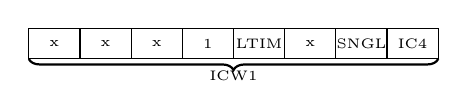
\begin{tikzpicture}[scale=0.65, every node/.style={font=\tiny, inner sep=0pt}]
    % Draw 8 boxes for bits
    \foreach \i in {0,...,7} {
        \draw (\i,0) rectangle ++(1,0.6);
    }
    % Bit labels (D7...D0)
    \foreach \i/\b in {0/x,1/x,2/x,3/1,4/LTIM,5/x,6/SNGL,7/IC4} {
        \node at (\i+0.5,0.3) {\b};
    }
    \draw [decorate,decoration={brace,amplitude=4pt,mirror},thick] (0,0) -- (8,0) node[midway,below=4pt, font=\tiny] {ICW1};
\end{tikzpicture}
\end{center}

\noindent
\begin{tabular}{@{}p{0.10\linewidth}p{0.22\linewidth}p{0.62\linewidth}@{}}
\hline
位 & 名称 & 含义 / 值 \\
\hline
D4 & 特征位 & 标识为 ICW1(启动初始化序列) \\
D3 & LTIM & 1:电平触发;0:边沿触发(上升沿) \\
D1 & SNGL & 1:单片工作(无 ICW3);0:级联(需 ICW3) \\
D0 & IC4  & 1:需要 ICW4;0:不需要 ICW4 \\
\hline
\end{tabular}

ICW1 写入必须通过偶地址端口($A_0 = 0$)。\red{8259A 物理上只有一根地址线 $A_0$},因而区分为:
\begin{itemize}
    \item \red{偶地址($A_0=0$)}:接收 ICW1、OCW2、OCW3。
    \item \red{奇地址($A_0=1$)}:接收 ICW2、ICW3、ICW4、OCW1。
\end{itemize}

ICW1 用于启动初始化序列并设定触发与级联等基本模式。

\green{\texttt{ICW2}}

\begin{center}
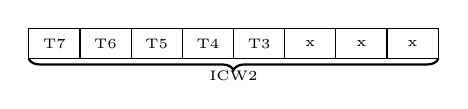
\begin{tikzpicture}[scale=0.65, every node/.style={font=\tiny, inner sep=0pt}]
    % Draw 8 boxes for bits
    \foreach \i in {0,...,7} {
        \draw (\i,0) rectangle ++(1,0.6);
    }
    % Bit labels (D7...D0)
    \foreach \i/\b in {0/T7,1/T6,2/T5,3/T4,4/T3,5/x,6/x,7/x} {
        \node at (\i+0.5,0.3) {\b};
    }
    \draw [decorate,decoration={brace,amplitude=4pt,mirror},thick] (0,0) -- (8,0) node[midway,below=4pt, font=\tiny] {ICW2};
\end{tikzpicture}
\end{center}


\concepttable{
    \conrow{作用}{设置\red{外部中断类型号的基值}(对应 IR0 的中断号)。}
    \conrow{位域}{D7--D3:由用户编程设定(中断向量的高 5 位);\quad D2--D0:初始化时通常为 \texttt{000},中断响应时由 8259A 根据 IR 编号 (0--7) 填入。}
    \conrow{向量计算}{中断向量 =(ICW2 的高 5 位)拼接(IR 的 3 位编号)。即 Vector = T7..T3 : IR2..IR0。}
    \conrow{示例}{例如 ICW2 = \texttt{08H}(二进制 \texttt{00001 000})或 \texttt{70H}(\texttt{01110 000}),其高 5 位分别为 \texttt{00001} 和 \texttt{01110}。}
}

\green{\texttt{ICW3}}

% ICW3:主/从片说明
\begin{center}
\begin{tikzpicture}[scale=0.65, every node/.style={font=\tiny, inner sep=0pt}]
    \foreach \i in {0,...,7} {
        \draw (\i,0) rectangle ++(1,0.6);
    }
    \foreach \i/\b in {0/D7,1/D6,2/D5,3/D4,4/D3,5/D2,6/D1,7/D0} {
        \node at (\i+0.5,0.3) {\b};
    }
    \draw [decorate,decoration={brace,amplitude=4pt,mirror},thick] (0,0) -- (8,0) node[midway,below=4pt, font=\tiny] {ICW3(主片):位掩码,位 i=1 表示从片连接到主片 IRi};
\end{tikzpicture}
\end{center}

当 ICW1 中的 SNGL=0(级联模式)时,主片须在 ICW3 中写入一个 8 位位掩码,位 i(0..7)置 1 表示该位对应的 IRi 引脚上连接有从片;其它位置 0。

\begin{center}
\begin{tikzpicture}[scale=0.65, every node/.style={font=\tiny, inner sep=0pt}]
    \foreach \i in {0,...,7} {
        \draw (\i,0) rectangle ++(1,0.6);
    }
    \foreach \i/\b in {0/x,1/x,2/x,3/x,4/x,5/D2,6/D1,7/D0} {
        \node at (\i+0.5,0.3) {\b};
    }
    \draw [decorate,decoration={brace,amplitude=4pt,mirror},thick] (0,0) -- (8,0) node[midway,below=4pt, font=\tiny] {ICW3(从片):低 3 位存从片 ID(0--7),高位无意义};
\end{tikzpicture}
\end{center}

从片的 ICW3 仅使用低 3 位存放该从片在主片上的 ID(0--7),高 5 位通常置 0。

\concepttable{
    \conrow{示例}{若某从片接在主片的 IR2:主片 ICW3 = 00000100B = 04H;该从片 ICW3 = 00000010B = 02H。}
}

\green{\texttt{ICW4}}

\begin{center}
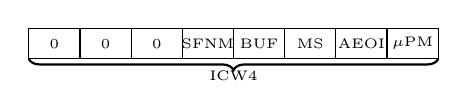
\begin{tikzpicture}[scale=0.65, every node/.style={font=\tiny, inner sep=0pt}]
    \foreach \i in {0,...,7} {
        \draw (\i,0) rectangle ++(1,0.6);
    }
    \foreach \i/\b in {0/0,1/0,2/0,3/SFNM,4/BUF,5/MS,6/AEOI,7/$\mu$PM} {
        \node at (\i+0.5,0.3) {\b};
    }
    \draw [decorate,decoration={brace,amplitude=4pt,mirror},thick] (0,0) -- (8,0) node[midway,below=4pt, font=\tiny] {ICW4};
\end{tikzpicture}
\end{center}


ICW4 为可选命令字(当 ICW1 的 D0=1 时需写入)。在 8086/8088 系统中常用,用于设置缓冲、自动 EOI 与微处理器工作模式(但是我们前面也没有整理这个,所以大抵是不重要的了)等。

\concepttable{
    \conrow{D4 — SFNM}{1: 特殊全嵌套(用于级联主片);\quad 0: 正常全嵌套}
    \conrow{D3 — BUF}{1: 缓冲模式;\quad 0: 非缓冲模式}
    \conrow{D2 — M/S}{在缓冲模式下有效:1 = 主片;\quad 0 = 从片}
    \conrow{D1 — AEOI}{1: 自动结束中断;\quad 0: 非自动(需软件发送 EOI)}
    \conrow{D0 — $\mu$PM}{1: 8086/8088 模式;\quad 0: MCS-80/85 模式}
}

\entry{\green{初始化编程总结}}{
    \concepttable{
        \conrow{单片模式}{
            写序:ICW1(偶地址 A0=0,启动初始化) → ICW2(奇地址,设定中断向量基值) →(若需要)ICW4(奇地址,设定 CPU 模式 / EOI 等)。
        }
        \conrow{级联模式(主片)}{
            写序:ICW1(偶) → ICW2(奇,基址) → ICW3(奇,标记连接的从片 IR 位) → ICW4(奇,微模式/缓冲/自动 EOI 等)。
        }
        \conrow{级联模式(从片)}{
            写序:ICW1(偶) → ICW2(奇,基址) → ICW3(奇,低 3 位为本从片 ID) → ICW4(奇)。
        }
    }
}
\entry{注}{
    主/从片须分别独立初始化:\textbf{仅 ICW1 写入偶地址端口(A0=0)},ICW2/ICW3/ICW4 均写入奇地址端口(A0=1)。
}


\green{初始化编程示例}

\entry{示例(PC/XT)}{
    \concepttable{
        \conrow{系统配置}{单片、边沿触发、向量基址 08H、非缓冲、非自动 EOI;端口 20H/21H。}
        \conrow{写序}{ICW1(偶地址端口) → ICW2(奇地址端口) → ICW4(奇地址端口)}
        \conrow{示例代码}{
            \texttt{MOV AL, 00010011B} \par
            \texttt{OUT 20H, AL} \par
            \texttt{MOV AL, 00001000B} \par
            \texttt{OUT 21H, AL} \par
            \texttt{MOV AL, 00000111B} \par
            \texttt{OUT 21H, AL}
        }
    }
}

\hlblue{\textbf{操作编程}}

运行时按需写入 OCW(操作命令字)以动态控制 8259A。

\concepttable{
    \conrow{OCW1}{用于操作 IMR(中断屏蔽寄存器),设置或修改中断屏蔽位。}
    \conrow{OCW2}{用于发送 EOI 并可设置/调整优先级循环。}
    \conrow{OCW3}{用于选择读取内部寄存器状态(IRR/ISR)或设置特殊屏蔽/读寄存器模式。}
}

\green{\texttt{OCW1}}

\begin{center}
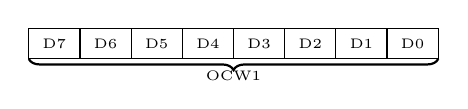
\begin{tikzpicture}[scale=0.65, every node/.style={font=\tiny, inner sep=0pt}]
    \foreach \i in {0,...,7} {
        \draw (\i,0) rectangle ++(1,0.6);
    }
    \foreach \i/\b in {0/D7,1/D6,2/D5,3/D4,4/D3,5/D2,6/D1,7/D0} {
        \node at (\i+0.5,0.3) {\b};
    }
    \draw [decorate,decoration={brace,amplitude=4pt,mirror},thick] (0,0) -- (8,0) node[midway,below=4pt, font=\tiny] {OCW1};
\end{tikzpicture}
\end{center}

OCW1 专门用于操作 \textbf{IMR(中断屏蔽寄存器)},用于设置哪些中断被\red{屏蔽(1)}或\red{允许(0)}。OCW1 必须写入\red{奇地址端口($A_0 = 1$)}。

\entry{\green{堂练 — 屏蔽单一中断线(IR4)}}{
    \concepttable{
        \conrow{题目条件}{
            在 IBM PC(8259A)系统中,8259A 的端口为 \texttt{20H}/\texttt{21H},要求仅屏蔽 \texttt{IR4},不改变其它中断屏蔽位。
        }
        \conrow{解题思路}{
            读出当前 IMR(OCW1),将 IR4 对应位(位 4)置 1,再写回以更新 IMR;为避免读-改-写期间的竞态可短暂禁止中断(\texttt{CLI})并在完成后恢复(\texttt{STI})。
        }
        \conrow{程序示例}{
            \texttt{CLI} \par
            \texttt{IN\ \ AL,\,21h} \par
            \texttt{OR\ \ AL,\,00010000b\ \ ; 设置位 4 (屏蔽 IR4)} \par
            \texttt{OUT\ \ 21h,\,AL} \par
            \texttt{STI}
        }
        \conrow{要点}{
            仅做读-改-写以保证其他位不被改变;在中断处理或多核并发环境下需谨慎处理中断使能状态并保存/恢复原状态。
        }
    }
}

\green{\texttt{OCW2}}

\begin{center}
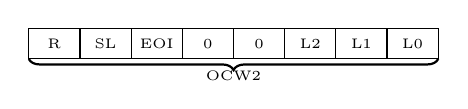
\begin{tikzpicture}[scale=0.65, every node/.style={font=\tiny, inner sep=0pt}]
    \foreach \i in {0,...,7} {
        \draw (\i,0) rectangle ++(1,0.6);
    }
    \foreach \i/\b in {0/R,1/SL,2/EOI,3/0,4/0,5/L2,6/L1,7/L0} {
        \node at (\i+0.5,0.3) {\b};
    }
    \draw [decorate,decoration={brace,amplitude=4pt,mirror},thick] (0,0) -- (8,0) node[midway,below=4pt, font=\tiny] {OCW2};
\end{tikzpicture}
\end{center}

\concepttable{
    \conrow{D7 — R}{1: 固定优先权;\quad 0: 循环优先权}
    \conrow{D6 — SL}{1: OCW2 最后 3 位有效;\quad 0: OCW2 最后 3 位无效}
    \conrow{D5 — EOI}{1: 发出 EOI(清除 ISR 中相应的服务位);\quad 0: 不发 EOI}
    \conrow{D4 - D3}{\red{特征位},均为 0}
    \conrow{D2 - D0}{与 EOI 一起使用时指定要结束的中断级号(0--7)。}
}

\green{\texttt{OCW3}}

\begin{center}
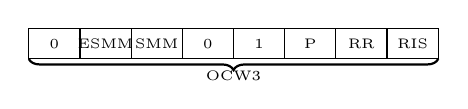
\begin{tikzpicture}[scale=0.65, every node/.style={font=\tiny, inner sep=0pt}]
    \foreach \i in {0,...,7} {
        \draw (\i,0) rectangle ++(1,0.6);
    }
    \foreach \i/\b in {0/0,1/ESMM,2/SMM,3/0,4/1,5/P,6/RR,7/RIS} {
        \node at (\i+0.5,0.3) {\b};
    }
    \draw [decorate,decoration={brace,amplitude=4pt,mirror},thick] (0,0) -- (8,0) node[midway,below=4pt, font=\tiny] {OCW3};
\end{tikzpicture}
\end{center}

OCW3 用于配置特殊屏蔽方式及查询模式。它与 OCW2 一样写入偶地址端口($A_0=0$),区分特征位为 $D_4=0,\;D_3=1$,主要功能为\red{切换/启用特殊屏蔽并选择读出内部寄存器(IRR/ISR)或进行查询(Poll)。}


\concepttable{
    \conrow{特殊屏蔽位(ESMM / SMM)}{
        ESMM:开启后使能 SMM 位效果;ESMM=0 时维持普通屏蔽。\par
        SMM:SMM=1 进入特殊屏蔽模式(允许低优先级中断中断高优先级,中断行为受限;用途少见);SMM=0 为普通屏蔽方式。
    }
    \conrow{查询命令(P)}{
        P=1:进入查询(Poll)模式,CPU 以程序查询方式读取状态时,8259A 返回是否有待处理中断的状态字,而不是中断向量号,便于轮询检测中断存在性。
    }
    \conrow{读取内部寄存器(RR / RIS)}{
        RR=1:启用读取内部寄存器功能。\par
        RIS=0:下一次读偶地址端口时返回 IRR(中断请求寄存器)。\par
        RIS=1:下一次读偶地址端口时返回 ISR(中断服务寄存器)。\par
        RR=0:取消读寄存器操作。
    }
}
\entry{查询方式(Poll)}{
    \concepttable{
        \conrow{触发条件}{CPU 向 8259A 写入 OCW3,设定 $P=1$,\red{紧接着执行一次 \texttt{IN} 指令},该 \texttt{IN} 被 8259A 解释为查询。}
        \conrow{功能}{CPU 主动询问 8259A 是否有待处理的中断请求;若有,8259A 在返回值中指示优先级最高的请求,否则返回“无请求”状态。}
    }
}


\section{第八章 常用接口技术}

\subsection{8255A}

\entry{8255 功能介绍}{
        \red{8255} 是一种\red{可编程的并行通信接口芯片},可用于 \red{CPU} 和外设之间进行并行数据传输。内部有\red{三个 8 位的数据端口},有三种工作方式。端口号的 \red{A0A1} 为 \red{00}、\red{01}、\red{10} 分别表示读写 \red{A、B、C 口};\red{11} 表示只写控制寄存器。
    }

\imgleft[0.3]{images/image-2025-12-26-00-05-16.png}{
    \entry{并行通信}{
        指\red{多位数据同时进行传送}的方式,其特点是\red{传输速度快}。
    }
        \concepttable{
            \conrow{方式 0}{基本的输入/输出方式,A/B/C 口均可用,C 口仅需设置方向。}
            \conrow{方式 1}{选通的输入/输出方式,A/B 口可用,支持中断方式传输,C 口部分引脚用于控制和中断信号。}
            \conrow{方式 2}{选通的双向传输方式,仅 A 口可用,支持双向传输和中断,C 口部分引脚用于控制和中断信号。}
        }
        \concepttable{
            \conrow{A 口}{可工作在方式 0、1、2,方式 2 时支持双向传输。}
            \conrow{B 口}{可工作在方式 0、1,仅支持单向传输。}
            \conrow{C 口}{只能工作在方式 0,高四位和低四位可分开使用,方式 1/2 时部分引脚用于控制和中断。}
        }
}
\red{方式 1、2}:选通输入输出方式,可以\red{中断方式传输},且\red{C 口会固定的引脚用作控制联络信号和中断请求信号}。\par
\red{仅 A 口工作在方式 2 时,可以双向传输},A 口工作在方式 0、1 及 B、C 口只能单向传输。\par
\entry{控制字}{
    控制字分为端口的\red{方式选择控制字}(可使 8255 的 3 个数据端口工作在不同的方式)和 C 口的\red{按位置位和复位控制字}(可使 C 口的任意一位置位和复位)。
    \red{★控制字送入的端口为最后一个端口}
}
\vspace{-0.3cm}
\begin{center}
\begin{tikzpicture}[scale=0.65, every node/.style={font=\tiny, inner sep=0pt}]
    % Draw 8 boxes for bits
    \foreach \i in {0,...,7} {
        \draw (\i,0) rectangle ++(1,0.6);
    }
    % Bit labels (D7...D0)
    \foreach \i/\b in {0/D7,1/D6,2/D5,3/D4,4/D3,5/D2,6/D1,7/D0} {
        \node at (\i+0.5,0.3) {\b};
    }
    % Value labels
    \node[red] at (0.5,0.85) {1};
    % Draw a brace and label
    \draw [decorate,decoration={brace,amplitude=4pt,mirror},thick] (0,0) -- (8,0) node[midway,below=4pt, font=\tiny] {方式控制字(8255A)};
\end{tikzpicture}
\end{center}
 
\subsection{8253}

\entry{概述}{
    ★\red{8253} 是一种\red{可编程的计数器/定时器接口芯片},最高计数频率为 \red{$2$MHz},可用于产生各种\red{定时波形},也可用于对\red{外部事件计数}。内部有\red{三个独立的 $16$ 位减一计数器}(互不干扰,支持\blue{二进制 (Binary) }或 \blue{二-十进制 (BCD码)} 计数),通过设置控制字,各计数器可以工作于 \red{$6$ 种工作方式}。
}
功能简述:

\imgleft[0.4]{images/image-2025-12-29-14-11-40.png}{

\concepttable{
    \conrow{CLK}{基准信号,即输入的\red{计数脉冲源}。所有输出变化均以此为时间基准。}
    \conrow{OUT1 (定时)}{启动后输出维持一段时间电平后跳变,用于产生确定的\red{时间延迟}。}
    \conrow{OUT2 (分频)}{输入信号频率较高,输出频率较低,输出周期是输入周期的\red{整数倍}。}
    \conrow{OUT3 (方波)}{分频的特殊形式,输出占空比为 \red{$50\%$},形成连续的\red{方波}。}
}

}

\imgleft[0.4]{images/image-2025-12-29-14-06-37.png}{

\entry{系统总线接口 (连接 CPU)}{
    \concepttable{
        \conrow{$D_7 \sim D_0$}{双向数据总线,用于 CPU 读写控制字或计数值。}
        \conrow{$\overline{CS}$}{片选信号,低电平有效,由地址译码电路产生。}
        \conrow{$\overline{RD} / \overline{WR}$}{读/写信号,低电平有效,控制数据传输方向。}
        \conrow{$A_1, A_0$}{端口选择:$00, 01, 10$ 分别对应计数器 $0, 1, 2$;$11$ 为控制寄存器。}
    }
}
\entry{计数通道信号 (连接外设)}{
    \concepttable{
        \conrow{$CLK_{0-2}$}{时钟输入,计数脉冲源,\red{下降沿}触发减 $1$ 操作。}
        \conrow{$GATE_{0-2}$}{门控输入,用于启动、停止或暂停计数过程。}
        \conrow{$OUT_{0-2}$}{输出信号,计数完成或达到条件时输出特定波形。}
    }
}

}

\entry{控制寄存器}{只能进行\red{写操作},不能读。CPU 通过向此寄存器写入“控制字”来设定各通道的工作方式。}

\entry{计数通道结构}{包含三个独立的计数通道(0、1、2),内部由以下三部分配合实现“预置 $\rightarrow$ 减计数 $\rightarrow$ 读出”逻辑:}
\concepttable{
    \conrow{初值寄存器 (CR)}{\red{16 位}。用于预置计数的起始值。}
    \conrow{执行部件 (CE)}{\red{16 位减法计数器}。在 $CLK$ 信号驱动下进行减 1 计数。}
    \conrow{输出锁存器 (OL)}{\red{16 位}。用于锁存当前计数值供 CPU 读取,不影响计数进行。}
}

\red{8253 没有状态寄存器},CPU \red{无法直接读取}状态寄存器来获知当前工作状态或回读控制字。这与具有状态回读功能的 \red{8254} 不同。

\noindent
\begin{minipage}[t]{0.38\linewidth}
    \entry{端口地址分配}{8253 占用 4 个 I/O 端口。CPU 通过 $A_1, A_0$ 选择:}
    \concepttable{
        \conrow{00}{计数通道 0}
        \conrow{01}{计数通道 1}
        \conrow{10}{计数通道 2}
        \conrow{11}{控制字寄存器}
    }
\end{minipage}
\hfill
\begin{minipage}[t]{0.58\linewidth}
    \entry{读写物理寄存器}{读写指向不同物理寄存器:}
    \concepttable{
        \conrow{写 (OUT)}{送入 \red{初值寄存器 (CR)}。}
        \conrow{读 (IN)}{来自 \red{输出锁存器 (OL)}。}
    }
    \tiny 这种“双缓冲”设计保证计数时读数稳定。
\end{minipage}
\par\vspace{2pt}

\noindent
\begin{minipage}[t]{0.49\linewidth}
    \entry{实例 1:连续地址 (8088)}{
        \concepttable{
            \conrow{设定}{地址范围:$0380H \sim 0383H$。地址连续(步长为 1)。}
            \conrow{分析}{$0380H (\dots 00) \rightarrow A_1A_0 = 00$ \par $0381H (\dots 01) \rightarrow A_1A_0 = 01$ \par $0382H (\dots 10) \rightarrow A_1A_0 = 10$ \par $0383H (\dots 11) \rightarrow A_1A_0 = 11$}
            \conrow{连接}{CPU 的 $A_1, A_0$ 直接连接到 8253 的 $A_1, A_0$。每一个逻辑地址都对应一个物理端口,无地址间隙。}
        }
    }
\end{minipage}
\hfill
\begin{minipage}[t]{0.49\linewidth}
    \entry{实例 2:偶地址对齐 (8086)}{
        \concepttable{
            \conrow{设定}{地址序列:$0380H, 0382H, \sim 0386H$ \par 只使用偶数地址。}
            \conrow{分析}{$0380H (\dots 00 \mathbf{0}) \rightarrow A_2A_1 = 00$;$0382H (\dots 01 \mathbf{0}) \rightarrow A_2A_1 = 01$;$0384H (\dots 10 \mathbf{0}) \rightarrow A_2A_1 = 10$;$0386H (\dots 11 \mathbf{0}) \rightarrow A_2A_1 = 11$。}
            \conrow{连接}{CPU $A_0$ 恒为 0。CPU 的 $A_2, A_1$ 错位连接到 8253 的 $A_1, A_0$。配合 16 位数据总线字节对齐要求。}
        }
    }
\end{minipage}

\entry{读/写逻辑真值表}{
    \concepttable{
        \conrow{片选前提}{所有操作必须在 $\overline{CS}=0$ 时有效。}
        \conrow{写 ($\overline{WR}=0$)}{根据 $A_1, A_0$ 写入通道 0/1/2 的计数初值寄存器,或写入控制字寄存器。}
        \conrow{读 ($\overline{RD}=0$)}{根据 $A_1, A_0$ 读取通道 0/1/2 的当前计数值。注意:\red{控制字寄存器只写不读}。}
    }
}

\entry{8 位总线与 16 位计数器接口}{
    8253 内部的计数初值寄存器 (CR) 和输出锁存器 (OL) 都是 16 位的,但外部数据总线 ($D_7 \sim D_0$) 只有 8 位。必须通过\red{两次 I/O 操作}来完成一个 16 位数据的传输,由控制寄存器中的控制字来指定读写顺序(如:先读/写低 8 位,再读/写高 8 位)。
}

\subsubsection{控制字}

\begin{center}
\begin{tikzpicture}[scale=0.65, every node/.style={font=\tiny, inner sep=0pt}]
    % Draw 8 boxes for bits
    \foreach \i in {0,...,7} {
        \draw (\i,0) rectangle ++(1,0.6);
    }
    % Bit labels (D7...D0)
    \foreach \i/\b in {0/D7,1/D6,2/D5,3/D4,4/D3,5/D2,6/D1,7/D0} {
        \node at (\i+0.5,0.3) {\b};
    }
    % Function labels
    \node at (0.5,0.85) {SC1}; \node at (1.5,0.85) {SC0};
    \node at (2.5,0.85) {RL1}; \node at (3.5,0.85) {RL0};
    \node at (4.5,0.85) {M2};  \node at (5.5,0.85) {M1}; \node at (6.5,0.85) {M0};
    \node at (7.5,0.85) {BCD};
    
    % Braces
    \draw [decorate,decoration={brace,amplitude=3pt},thick] (0,1) -- (2,1) node[midway,above=2pt] {计数器选择};
    \draw [decorate,decoration={brace,amplitude=3pt},thick] (2,1) -- (4,1) node[midway,above=2pt] {读写操作};
    \draw [decorate,decoration={brace,amplitude=3pt},thick] (4,1) -- (7,1) node[midway,above=2pt] {工作方式};
    \draw [decorate,decoration={brace,amplitude=3pt},thick] (7,1) -- (8,1) node[midway,above=2pt] {计数制};
    
    % Bottom label
    \node at (4,-0.4) {8253 控制字格式};
\end{tikzpicture}
\end{center}

\concepttable{
    \conrow{$SC_1, SC_0$}{
        \textbf{计数器选择}。因共用端口(3 个计数器共用一个控制端口),需指定目标通道。\par
        \red{00}: CNT0; \red{01}: CNT1; \red{10}: CNT2; \red{11}: 非法。
    }
    \conrow{$RL_1, RL_0$}{
        \textbf{读写格式}。定义 CR/OL 的读写位宽及顺序。\par
        \red{00}: \textbf{锁存命令} (不停止计数读取); \red{01}: 仅低8位; \red{10}: 仅高8位; \red{11}: \textbf{先低后高} (16位常用)。
    }
    \conrow{$M_2 \sim M_0$}{
        \textbf{工作方式}。设定方式 0 $\sim$ 5。
    }
    \conrow{$BCD$}{
        \textbf{计数制}。\red{0}: 二进制 ($FFFFH$); \red{1}: BCD码 ($9999$)。
    }
}

\noindent
\begin{minipage}[t]{0.49\linewidth}
    \entry{实例 1:8 位读写模式}{
        \blue{需求}:计数器 0,方式 2,仅使用低 8 位,初值 100,二进制计数。地址:$70H \sim 73H$。
    }
    \concepttable{
        \conrow{SC}{\red{00} (选择计数器 0)}
        \conrow{RL}{\red{01} (只读/写低 8 位)}
        \conrow{M}{\red{010} (方式 2,分频器)}
        \conrow{BCD}{\red{0} (二进制计数)}
        \conrow{控制字}{$00010100B = \red{14H}$}
    }
    \blue{汇编实现}:
    \begin{itemize}
        \item \texttt{MOV AL, 14H}
        \item \texttt{OUT 73H, AL \ \ ;写控制字}
        \item \texttt{MOV AL, 100 \ \ ;初值 100}
        \item \texttt{OUT 70H, AL \ \ ;写低 8 位}
    \end{itemize}
\end{minipage}
\hfill
\begin{minipage}[t]{0.49\linewidth}
    \entry{实例 2:16 位读写模式}{
        \blue{需求}:计数器 1,方式 1,16 位 (先低后高),初值 1234,BCD 码。地址:$70H \sim 73H$。
    }
    \concepttable{
        \conrow{SC}{\red{01} (选择计数器 1)}
        \conrow{RL}{\red{11} (先低 8 位后高 8 位)}
        \conrow{M}{\red{001} (方式 1,单稳态)}
        \conrow{BCD}{\red{1} (BCD 码计数)}
        \conrow{控制字}{$01110011B = \red{73H}$}
    }
    \blue{汇编实现}:
    \begin{itemize}
        \item \texttt{MOV AL, 73H}
        \item \texttt{OUT 73H, AL \ \ ;写控制字}
        \item \texttt{MOV AX, 1234H \ ;BCD 码初值}
        \item \texttt{OUT 71H, AL \ \ ;写低 8 位}
        \item \texttt{MOV AL, AH}
        \item \texttt{OUT 71H, AL \ \ ;写高 8 位}
    \end{itemize}
\end{minipage}

\entry{锁存命令}{解决在计数器运行过程中读取数值不稳定的问题。通过向控制寄存器写入 $RL_1RL_0 = 00$ 的控制字,将当前计数值复制到 \red{输出锁存器 (OL)} 中保持不变,而 \red{执行部件 (CE)} 继续计数。}

\entry{锁存读出示例}{
    \concepttable{
    \conrow{锁存机制}{向控制口发送控制字,其中 $RL_1RL_0 = 00$。8253 接收后锁存当前值,不影响内部计数。}
    \conrow{实例分析}{读取计数器 0 当前值:$SC=00, RL=00$,其余位无关,控制字为 \red{00H}。}
    \conrow{代码流程}{
        1. \texttt{MOV AL, 00H} \par
        2. \texttt{OUT 73H, AL} (向控制口发送锁存命令) \par
        3. \texttt{IN AL, 70H} (从数据口读取低 8 位) \par
        4. \texttt{IN AL, 70H} (从数据口读取高 8 位)
    }
    \conrow{注意}{读出操作必须符合初始化时设定的 \red{RL} 格式(如 16 位模式需连读两次)。}
    }
}

\entry{相关名词解释}{
    \concepttable{
    \conrow{CLK 脉冲}{指 \red{CLK} 引脚上的信号单元。在计数过程中,每一个 \red{CLK} 脉冲的\red{下降沿}到来时,计数器减 1。}
    \conrow{计数器}{与“计数通道”同义}
    \conrow{时常数}{指通过指令写入计数器的值,等同于\red{初值}。输出波形的周期或延时由该值决定:$\text{时间} = \text{初值} \times T_{CLK}$。}
    }
}

\subsubsection{方式 0}

\entry{功能定义}{
    主要用于\red{定时中断}。给定时间 $t_0$,到达后输出信号通知 CPU。
}

\noindent
\begin{minipage}[t]{0.55\linewidth}
    \concepttable{
        \conrow{初始化}{写入方式控制字后,输出引脚 \red{OUT 变为低电平}。}
        \conrow{计数过程}{写入初值后开始减 1 计数,期间 \red{OUT 保持低电平}。}
        \conrow{计数结束}{当计数值减到 0 时,\red{OUT 立即跳变为高电平}。产生的\red{上升沿信号}通常连接 CPU 中断请求引脚。}
    }
\end{minipage}%
\hfill
\begin{minipage}[t]{0.44\linewidth}
    \red{GATE} 是硬件门控信号,在方式 0 中充当“计数使能开关”:
    
    \concepttable{
        \conrow{0}{暂停计数,计数器保持当前值不变,忽略 CLK 脉冲。}
        \conrow{1}{允许计数,计数器正常工作。}
    }
\end{minipage}

\imgleft[0.4]{images/image-2025-12-29-15-24-32.png}{
    \entry{时序分析 (基本过程)}{
        重点在于 \red{$N+1$} 个时钟周期的由来。
        \concepttable{
            \conrow{写入控制字}{$\overline{WR}$ 有效 $\to$ \red{OUT 变低} (起始状态)。}
            \conrow{写入初值}{第二个 $\overline{WR}$ 将初值 $N$ 写入 CR。}
            \conrow{载入时刻}{写入后第 1 个 CLK 下降沿,数据 CR $\to$ CE。}
            \conrow{计数过程}{载入后开始减 1 ($N \to 0$)。总时长 \red{$N+1$} 个 CLK。}
            \conrow{终值输出}{CE 减为 0 时,\red{OUT 变高}。}
        }
    }
}

\imgleft[0.4]{images/image-2025-12-29-15-19-48.png}{
    \entry{GATE 控制 (暂停)}{
        \concepttable{
            \conrow{GATE=0}{暂停计数 (CE 保持),OUT 保持低。}
            \conrow{GATE=1}{恢复计数 (从暂停值继续)。}
        }
    }
    \entry{结论}{利用 GATE 可\red{加长 OUT 低电平宽度}。实际时间 = 预置 + 暂停。}
}

\imgleft[0.4]{images/image-2025-12-29-15-22-52.png}{
    \entry{重写初值 (重启动)}{
        若在计数未结束时写入新初值,8253 会放弃当前进程,在下一个 CLK \red{重新装入新初值并重新开始}。同样实现了\red{加长 OUT 低电平宽度}的效果。
    }
    \entry{周期数}{写入时常数为 $N$ 时,OUT 低电平宽度为 \red{$N+1$} 个 CLK 周期。}
    \entry{计数完成后}{CE 寄存器会变成FFFFH,OUT(OL 锁存器)一直输出高电平,但是 CE 持续在-1 计数}
}

\entry{方式 0 编程示例}{
    已知端口 $40H \sim 43H$,计数器 0,方式 0,初值 1500,二进制计数。
}
\concepttable{
    \conrow{控制字}{SC=00, RL=11, M=000, BCD=0 $\to$ \red{30H}}
    \conrow{时常数}{$1500 = 05DCH$ (低位 \red{DCH},高位 \red{05H})}
}
\blue{汇编实现}:
\begin{itemize}
    \item \texttt{MOV DX, 43H \ \ ;指向控制口}
    \item \texttt{MOV AL, 30H \ \ ;写控制字}
    \item \texttt{OUT DX, AL}
    \item \texttt{MOV DX, 40H \ \ ;指向计数器 0 数据口}
    \item \texttt{MOV AX, 1500 \ ;AX = 05DCH}
    \item \texttt{OUT DX, AL \ \ ;写低 8 位 (DCH)}
    \item \texttt{MOV AL, AH \ \ ;取高 8 位 (05H)}
    \item \texttt{OUT DX, AL \ \ ;写高 8 位}
\end{itemize}
\entry{核心逻辑}{
    写初值 $\to$ OUT 低 $\to$ 计数 $\to$ 0 $\to$ OUT 高。\red{定时时长 $= (N+1) \times T_{CLK}$。}可通过 GATE 硬件信号暂停,或重写初值延长定时。
}

\subsubsection{方式 1}

\entry{功能定义}{
    \red{单脉冲形成}。即产生一个宽度可控的\red{负脉冲}。

    \concepttable{
        \conrow{触发源}{\red{硬件触发}。区别于方式 0 的软件写入触发,方式 1 必须由 \red{GATE} 引脚的\red{上升沿}(由低电平变高电平)来触发。}
        \conrow{脉冲宽度}{输出负脉冲的宽度为 \red{$N \times T_{CLK}$},其中 $N$ 为预置的初值。}
    }

}

\imgleft[0.4]{images/image-2025-12-29-15-43-06.png}{

    \concepttable{
        \conrow{初始化}{写入方式控制字后 \red{OUT 变高};写入初值后 OUT 保持高电平。}
        \conrow{触发时刻}{\red{GATE 上升沿}触发。在随后的下一个 CLK 下降沿,OUT 由高变低。}
        \conrow{计数与结束}{计数器减 1 期间 OUT 为低;减至 0 时 OUT 跳变为高。低电平宽度 $= N \times T_{CLK}$。}
    }
    \entry{可重触发性}{
        在脉冲未结束时,若 \red{GATE 再次出现上升沿},8253 会在下一个 CLK 将初值寄存器 (CR) 的值\red{重新装入}执行单元 (CE),使计数器重新开始,从而\red{延长 OUT 低电平宽度}。
    }

}

\imgleft[0.4]{images/image-2025-12-29-15-43-35.png}{

\entry{修改初值 (方式 1)}{在脉冲输出过程中,若 CPU 修改计数初值:}
\concepttable{
    \conrow{系统响应}{新初值 $N_{new}$ 仅存入 \red{初值寄存器 (CR)}。当前计数器 (CE) 不受影响,继续按旧值 $N_{old}$ 减至 0,当前脉冲宽度不变。}
    \conrow{生效时刻}{仅在 \red{下一次 GATE 上升沿} 到来时,新值 $N_{new}$ 才从 CR 装入 CE。}
    \conrow{结论}{写入新初值\red{不会立即重启}计数,而是预置给下一次触发使用。}
}

}


\noindent{\setlength{\tabcolsep}{2pt}
    \begin{tabular}{@{}p{0.48\linewidth}|p{0.48\linewidth}@{}}
    \hline
    \centering \blue{方式 0 (软件触发)} & \centering \blue{方式 1 (硬件触发)} \tabularnewline \hline
    写初值操作直接启动计数 & GATE 上升沿触发启动 \\
    GATE \red{电平}敏感:1 计数,0 暂停 & GATE \red{边沿}敏感:上升沿重触发 \\
    低电平宽度为 \red{$N+1$} 个 CLK & 低电平宽度为 \red{$N$} 个 CLK \\ \hline
    \end{tabular}}
    \concepttable{
    \conrow{相同点}{均为减 1 计数;工作时输出低电平;均具备定时功能。}
}

\noindent
\begin{minipage}[t]{0.49\linewidth}
    \entry{实例 1-单一通道编程}{\par
        \blue{需求}:计数器 2,方式 1,初值 15,仅低 8 位。地址:控制口 \red{COUNTD},计数器 2 \red{COUNTC}。
    }
    \concepttable{
        \conrow{控制字}{$SC=10, RL=01, M=001, BCD=0 \to \red{92H}$}
        \conrow{汇编实现}{
            \texttt{MOV AL, 92H} \par
            \texttt{OUT COUNTD, AL \ ;写控制字} \par
            \texttt{MOV AL, 15} \par
            \texttt{OUT COUNTC, AL \ ;写初值}
        }
    }
\end{minipage}
\hfill
\begin{minipage}[t]{0.49\linewidth}
    \entry{实例 2-波形分析与混合}{\par
        \blue{需求}:根据波形反推。OUT0 为方式 0,OUT1 为方式 1。初值均为 7。
    }
    \concepttable{
        \conrow{CNT0 控制字}{$SC=00, RL=01, M=000 \to \red{10H}$}
        \conrow{CNT1 控制字}{$SC=01, RL=01, M=001 \to \red{52H}$}
        \conrow{汇编实现}{
            \texttt{MOV AL, 10H; OUT COUNTD, AL} \par
            \texttt{MOV AL, 52H; OUT COUNTD, AL} \par
            \texttt{MOV AL, 7} \par
            \texttt{OUT COUNTA, AL \ ;CNT0 初值} \par
            \texttt{OUT COUNTB, AL \ ;CNT1 初值}
        }
    }
\end{minipage}

\subsubsection{方式 2}

\entry{功能定义}{
    分频脉冲形成。作为 \red{$N$ 分频器}使用,产生\red{连续的、周期性的}负脉冲。每输入 $N$ 个时钟脉冲,输出 $1$ 个低电平脉冲。
}

\noindent
\begin{minipage}[t]{0.49\linewidth}
\vspace{-0.2cm}
\concepttable{
    \conrow{初始化}{写入控制字后 \red{OUT 立即变高}。写入初值 $N$ 后,在下一个 CLK 下降沿将初值装入执行单元 (CE)。}
    \conrow{计数过程}{计数器从 $N$ 开始递减。在 $N$ 减至 $1$ 期间,\red{OUT 保持高电平}。}
    \conrow{关键跳变}{当计数值减到 \red{$1$} 时(注意不是 $0$),\red{OUT 跳变为低电平},并维持 $1$ 个时钟周期 ($T_{CLK}$)。}
    \conrow{自动重装}{经过 $1$ 个周期的低电平后,\red{计数器自动重新装入初值 $N$,OUT 恢复高电平,开始新一轮计数。}}
}

\end{minipage}
\hfill
\begin{minipage}[t]{0.49\linewidth}

\entry{结论}{
    方式 2 输出的是周期信号,周期 $T = N \times T_{CLK}$。其中高电平持续 $N-1$ 个周期,低电平持续 $1$ 个周期。
}
\vspace{0.5cm}
\entry{GATE 硬件控制}{
    \concepttable{
        \conrow{GATE=1}{允许计数,正常执行分频功能。}
        \conrow{GATE=0}{禁止计数。若在计数过程中变低,OUT 立即变高;恢复为 $1$ 后,计数器将\red{重新装入初值}开始计数。}
    }
}

\end{minipage}

\entry{分频}{
        输出信号频率 $f_{out} = f_{in} / N$。
}

\imgleft[0.4]{images/image-2025-12-31-18-50-39.png}{

    \concepttable{
        \conrow{启动阶段}{$\overline{WR}$ 写入初值 $N$。下一个 CLK 下降沿,CE 载入 $N$,OUT 保持高电平。}
        \conrow{计数阶段}{CLK 驱动 CE 递减 ($N \to \dots \to 1$)。当 \red{CE=1} 时,\red{OUT 变为低电平}。}
        \conrow{循环阶段}{维持 $1$ 个 CLK 低电平后,CE 自动重装初值 $N$,OUT 恢复高电平,周而复始形成连续脉冲。}
    }

}

\imgleft[0.4]{images/image-2025-12-31-18-55-24.png}{
    \entry{GATE 信号控制与硬件同步}{
        方式 2 下,外部硬件信号 \red{GATE} 对计数过程具有控制和同步作用。
    }
    \concepttable{
        \conrow{GATE=0}{强制停止。计数器停止计数,\red{OUT 强制变为高电平}(若当前为低则立即拉高)。}
        \conrow{GATE=1}{允许计数,正常执行分频。}
        \conrow{GATE 上升沿}{触发\red{硬件同步}。无论当前计数值,立即在下一个 CLK \red{重新装入初值 $N$,从头开始计数}。常用于使计数周期与外部信号对齐。}
    }
}

\imgleft[0.4]{images/image-2025-12-31-18-57-39.png}{

    \entry{修改初值}{
        在计数过程中,若 CPU 通过软件修改计数初值:
    }
    \concepttable{
        \conrow{本次周期}{新初值仅存入 \red{初值寄存器 (CR)}。执行单元 (CE) 仍按旧值继续计数,直到完成当前周期(含低电平脉冲),不会出现“半截”脉冲。}
        \conrow{生效时刻}{在当前周期结束、触发\red{自动重装}时,新值才从 CR 装入 CE。}
        \conrow{对比方式 0}{方式 0 写入即生效(立即重启);方式 2 写入后\red{下周期生效},确保输出波形的完整性。}
    }

}

\entry{方式 2 特性总结}{

    \concepttable{
        \conrow{初始状态}{写入控制字后,\red{OUT 立即变为高电平}。}
        \conrow{启动时机}{写入初值后的下一个 \red{CLK} 下降沿,初值装入 \red{CE} 并开始减 1 计数。}
        \conrow{输出波形}{当计数减至 \red{1} 时,输出一个宽度为 \red{1 个 $T_{CLK}$} 的负脉冲。}
        \conrow{分频特性}{输出为连续周期信号,周期 \red{$T = N \times T_{CLK}$},频率 \red{$f_{out} = f_{in} / N$}。}
        \conrow{同步方式}{\blue{软件同步}:写入新初值,当前周期结束后生效;\blue{硬件同步}:\red{GATE 上升沿}触发立即重装初值并重新开始。}
        \conrow{GATE 逻辑}{\red{0}:停止计数且 \red{OUT} 变高;\red{1}:允许计数。}
    }

}

\subsubsection{方式 2 - 编程实例}

\entry{实例:5 分频器}{
    \blue{需求}:计数器 1,方式 2,初值 5,二进制,仅低 8 位。
}
\concepttable{
    \conrow{控制字}{SC=01, RL=01, M=010, BCD=0 $\to$ \red{54H}}
    \conrow{汇编实现}{
        \texttt{MOV AL, 54H} \par
        \texttt{OUT COUNTD, AL \ ;写控制字} \par
        \texttt{MOV AL, 5} \par
        \texttt{OUT COUNTB, AL \ ;写初值}
    }
}

\entry{波形特征}{
    总周期 $= N = 5$ 个 $T_{CLK}$;高电平持续 $N-1 = 4$ 个周期;低电平持续 $1$ 个周期。OUT1 在 $05, 04, 03, 02$ 期间为高,在 $01$ 期间为低,然后循环。
}

\subsubsection{方式 2 - 时常数计算}

\blue{频率已知}:$N = \dfrac{f_{in}}{f_{out}}$

\blue{周期已知}:$N = \dfrac{T_{out}}{T_{in}}$

\noindent
\begin{minipage}[t]{0.32\linewidth}
    \entry{实例 1}{
        \blue{已知}:$f_{in} = 2$ MHz,$f_{out} = 1$ kHz
    }
    \concepttable{
        \conrow{计算}{$N = \dfrac{2 \times 10^6}{1 \times 10^3}$\par
        $= \red{2000}$}
    }
\end{minipage}%
\hfill
\begin{minipage}[t]{0.32\linewidth}
    \entry{实例 2}{
        \blue{已知}:$T_{in} = 1\ \mu$s,$T_{out} = 1.3$ ms
    }
    \concepttable{
        \conrow{计算}{$1.3$ ms $= 1300\ \mu$s \par 
        \vspace{3pt}
        $N = \dfrac{1300}{1} = \red{1300}$}
    }
\end{minipage}%
\hfill
\begin{minipage}[t]{0.32\linewidth}
    \entry{实例 3}{
        \blue{已知}:$f_{in} = 1$ MHz ($T_{in} = 1\ \mu$s)
    }
    \concepttable{
        \conrow{波形图}{低电平 1.5 ms,高 3 ms}
        \conrow{计算}{$T_{out} = 4.5$ ms $= 4500\ \mu$s \par $N = \red{4500}$}
    }
\end{minipage}

\subsubsection{方式 3}

\entry{功能定义}{
    \red{方波信号发生器}。与方式 2 类似,也是一种分频器,但输出对称或近似对称的方波。输出信号周期 $T_{out} = N \times T_{CLK}$。
}

\noindent
\begin{minipage}[t]{0.49\linewidth}

    \img[\linewidth]{images/image-2025-12-31-20-50-11.png}

    \concepttable{
        \conrow{N 为偶数}{输出\red{完全对称}方波。高电平持续 $N/2$ 个 $T_{CLK}$,低电平持续 $N/2$ 个 $T_{CLK}$。}
        \conrow{N 为奇数}{输出\red{近似对称}方波。高电平持续 $(N+1)/2$ 个 $T_{CLK}$,低电平持续 $(N-1)/2$ 个 $T_{CLK}$。}
    }

\end{minipage}
\hfill
\begin{minipage}[t]{0.49\linewidth}

    \img[\linewidth]{images/image-2025-12-31-20-51-26.png}
    \vspace{4pt}
    \entry{GATE 硬件控制}{
        与方式 2 逻辑一致:
        \concepttable{
            \conrow{GATE=1}{允许计数,正常输出方波。}
            \conrow{GATE=0}{禁止计数,\red{OUT 立即跳变为高电平}。}
            \conrow{GATE 上升沿}{触发硬件同步,使计数器\red{重新装入初值}开始计数。}
        }   
    }

\end{minipage}

\entry{修改初值}{
    在计数过程中写入新初值,不会立即影响当前输出。新初值将在\red{当前半个周期(高电平或低电平)结束}、发生电平跳变时装入执行单元。
}

\noindent
\begin{minipage}[t]{0.49\linewidth}

    \img[\linewidth]{images/image-2025-12-31-20-56-48.png}

    \entry{方式 3 偶数计数逻辑}{
        当计数初值 $N$ 为偶数时,8253 内部执行单元 (CE) 采用\red{减 2 计数}方式以实现对称方波。
    }
    \concepttable{
        \conrow{初始化}{写入方式 3 控制字后,\red{OUT 端初始为高电平}。}
        \conrow{前半周期 (高)}{写入偶数初值 $N$ 后,CE 从 $N$ 开始每隔一个 CLK \red{减 2}。当 $CE=0$ 时,OUT 翻转为低,\red{并自动重装初值 $N$}。}
        \conrow{后半周期 (低)}{CE 再次从 $N$ 开始每脉冲\red{减 2}。当 $CE=0$ 时,OUT 翻转为高,并再次重装初值 $N$。}
        \conrow{波形特征}{高低电平宽度相等,均为 $(N/2) \times T_{CLK}$,输出为\red{完全对称方波}。}
    }

\end{minipage}%
\hfill
\begin{minipage}[t]{0.49\linewidth}

    \img[\linewidth]{images/image-2025-12-31-21-02-18.png}

    \entry{方式 3 奇数计数逻辑}{
        当初值 $N$ 为奇数时,8253 内部通过修正逻辑处理不对称性。
    }
    \vspace{0.65cm}
    \concepttable{
        \conrow{第一阶段 (高)}{装入时硬件自动将 $N$ 修正为偶数 $N-1$,并进行“减 2”计数。实际输出高电平时间为 $(N+1)/2 \times T_{CLK}$(由于修正周期的存在)。}
        \conrow{第二阶段 (低)}{计数器重新装入修正后的偶数 $N-1$,进行“减 2”计数。实际输出低电平时间为 $(N-1)/2 \times T_{CLK}$。}
    }

\end{minipage}

\noindent
\begin{minipage}[t]{0.49\linewidth}

    \img[\linewidth]{images/image-2025-12-31-20-56-48.png}

    \entry{方式 3 偶数初值时序分析 ($N=4$)}{
     
        \concepttable{
            \conrow{初始化}{写入控制字后,\red{OUT} 端初始化为高电平。}
            \conrow{写入初值}{通过 $\overline{WR}$ 信号的负脉冲将初值 \red{$N=4$} 写入。}
            \conrow{启动延迟}{写入初值后的下一个 \red{CLK} 下降沿,计数器正式开始工作。}
            \conrow{计数逻辑}{执行单元 (CE) 采用 \red{减 2} 方式变化:$04 \to 02 \to 00$。}
            \conrow{波形输出}{CE 递减期间 \red{OUT 保持高电平} (2 个周期);减至 $00$ 后,OUT 变低,CE 自动重装为 $04$ 并再次减至 $00$,此时 \red{OUT 保持低电平} (2 个周期)。}
        }

    }

    \entry{应用场景}{方式 3 模式非常适合生成\red{低频时钟信号},例如将系统高频晶振分频后提供给低速外设使用。}

\end{minipage}%
\hfill
\begin{minipage}[t]{0.49\linewidth}

\img[\linewidth]{images/image-2025-12-31-21-02-18.png}

\vspace{3pt}

\entry{方式 3 奇数初值时序分析 ($N=5$)}{
    \concepttable{
        \conrow{高电平阶段}{宽度为 \red{3} 个 $T_{CLK}$。内部状态:$04 \to 02 \to 00$。对应 $(N+1)/2$。}
        \conrow{低电平阶段}{宽度为 \red{2} 个 $T_{CLK}$。内部状态:$04 \to 02$。对应 $(N-1)/2$。}
        \conrow{波形特征}{高电平比低电平宽一个时钟周期,形成\red{近似对称}的方波。}
    }
}

\end{minipage}

\entry{方式 3 特性总结}{
    \concepttable{
        \conrow{初始状态}{写入控制字后,\red{OUT} 立即变高。}
        \conrow{偶数初值 $N$}{高电平 $N/2$,低电平 $N/2$,输出\red{完全对称}方波。}
        \conrow{奇数初值 $N$}{高电平 $(N+1)/2$,低电平 $(N-1)/2$,输出\red{近似对称}方波。}
        \conrow{功能本质}{产生周期为 $N$ 的方波(即 \red{$N$ 分频})。}
        \conrow{软件同步}{写入新初值后,不立即打断当前半周期,需等待当前半周期结束后在下一次翻转重装时生效。}
        \conrow{硬件同步}{\red{GATE 上升沿}触发,立即复位计数器并从高电平周期的起始点重新计数(相位同步)。}
        \conrow{GATE 控制}{\red{0}:计数停止,\red{OUT 保持当前电平不变}(注意:方式 2 是强制变高);\red{1}:允许工作。}
    }
}

\entry{\hlblue{方式 3 编程示例 01:基本设计}}{
    \blue{场景}:8254 计数器 0 连接 CPU 的 \red{5 MHz} 时钟,输出 \red{0.5 MHz} 方波。
}

\concepttable{
    \conrow{参数计算}{输入频率 $f_{in} = 5$ MHz;输出频率 $f_{out} = 0.5$ MHz;分频系数 $N = f_{in}/f_{out} = 5/0.5 = \red{10}$。}
    \conrow{控制字}{SC=00, RL=01 (低 8 位), M=011 (方式 3), BCD=0 $\to$ \red{16H}}
    \conrow{汇编实现}{
        \texttt{MOV DX, COUNTD} \par
        \texttt{MOV AL, 16H} \par
        \texttt{OUT DX, AL \ \ ;写控制字} \par
        \texttt{MOV DX, COUNTA} \par
        \texttt{MOV AL, 10} \par
        \texttt{OUT DX, AL \ \ ;写初值}
    }
}

\entry{波形特征}{
    $N=10$ 为偶数,输出\red{完全对称方波}。高电平持续 $5$ 个 $T_{CLK}$,低电平持续 $5$ 个 $T_{CLK}$。周期 $T_{out} = 10 \times 0.2\ \mu\text{s} = 2\ \mu\text{s}$,对应频率 $0.5$ MHz。
}

\entry{\hlblue{方式 3 - 编程示例 02:级联方案}}{

\entry{级联设计题目}{
    \blue{系统配置}:8086 CPU 主频为 \red{5 MHz}。
    
    \blue{任务要求}:
    \concepttable{
        \conrow{任务 A}{计数器 0 输出 \red{1 MHz} 方波。}
        \conrow{任务 B}{计数器 2 产生 \red{1 Hz} 的单脉冲周期信号。}
    }
}

\noindent
\begin{minipage}[t]{0.33\linewidth}
    \entry{\hlred{级联方式 1:串行级联}}{

        \entry{硬件连接逻辑}{
            \concepttable{
                \conrow{计数器 1}{输入:\red{5 MHz} 系统时钟;初值:$N_1=5000$;输出:\red{1 kHz}。}
                \conrow{计数器 2}{输入:来自计数器 1 的输出 (\red{1 kHz});初值:$N_2=1000$;输出:\red{1 Hz}。}
            }
        }

        \entry{关键连接}{
            计数器 1 的 \red{OUT1} $\to$ 计数器 2 的 \red{CLK2}。
        }

        \entry{编程实现}{
            \concepttable{
                \conrow{计数器 1}{控制字:\red{76H};初值:\red{5000}。}
                \conrow{计数器 2}{控制字:\red{B4H};初值:\red{1000}。}
            }
        }

        \blue{汇编代码}:
        \begin{itemize}
            \item \texttt{MOV AL, 76H}
            \item \texttt{OUT COUNTD, AL}
            \item \texttt{MOV AL, B4H}
            \item \texttt{OUT COUNTD, AL}
            \item \texttt{MOV AX, 5000}
            \item \texttt{OUT COUNTB, AL}
            \item \texttt{MOV AL, AH}
            \item \texttt{OUT COUNTB, AL}
            \item \texttt{MOV AX, 1000}
            \item \texttt{OUT COUNTC, AL}
            \item \texttt{MOV AL, AH}
            \item \texttt{OUT COUNTC, AL}
        \end{itemize}

    }
\end{minipage}%
\hfill
\begin{minipage}[t]{0.33\linewidth}
    \entry{\hlred{级联方式 2:并行输入}}{

        \entry{硬件连接逻辑}{
            \concepttable{
                \conrow{计数器 0}{输入:\red{5 MHz};初值:$N_0=5$;输出:\red{1 MHz}(任务 A)。}
                \conrow{计数器 1}{输入:\red{5 MHz}(并行);初值:$N_1=5000$;输出:\red{1 kHz}。}
                \conrow{计数器 2}{输入:来自计数器 1 (\red{1 kHz});初值:$N_2=1000$;输出:\red{1 Hz}(任务 B)。}
            }
        }

        \entry{关键连接}{
            计数器 0 与 1-2 组并行;计数器 1 的 \red{OUT1} $\to$ 计数器 2 的 \red{CLK2}。
        }

        \entry{编程实现}{
            \concepttable{
                \conrow{计数器 0}{控制字:\red{16H};初值:\red{5}。}
                \conrow{计数器 1}{控制字:\red{76H};初值:\red{5000}。}
                \conrow{计数器 2}{控制字:\red{B4H};初值:\red{1000}。}
            }
        }

        \blue{汇编代码}:
        \begin{itemize}
            \item \texttt{MOV AL, 16H}
            \item \texttt{OUT COUNTD, AL}
            \item \texttt{MOV AL, 76H}
            \item \texttt{OUT COUNTD, AL}
            \item \texttt{MOV AL, B4H}
            \item \texttt{OUT COUNTD, AL}
            \item \texttt{MOV AL, 5}
            \item \texttt{OUT COUNTA, AL}
            \item \texttt{MOV AX, 5000}
            \item \texttt{OUT COUNTB, AL}
            \item \texttt{MOV AL, AH}
            \item \texttt{OUT COUNTB, AL}
            \item \texttt{MOV AX, 1000}
            \item \texttt{OUT COUNTC, AL}
            \item \texttt{MOV AL, AH}
            \item \texttt{OUT COUNTC, AL}
        \end{itemize}

    }
\end{minipage}
\hfill
\begin{minipage}[t]{0.33\linewidth}

\entry{\hlred {级联方式3:完全串联级联}}{
    
    \entry{硬件连接逻辑}{
        充分利用计数器 0 的中间成果,形成 \red{C0 $\to$ C1 $\to$ C2} 的全级联结构。
        \concepttable{
            \conrow{计数器 0}{输入:\red{5 MHz};初值:$N_0=5$;输出:\red{1 MHz}(任务 A)。}
            \conrow{计数器 1}{输入:来自计数器 0 (\red{1 MHz});初值:$N_1=1000$;输出:\red{1 kHz}。}
            \conrow{计数器 2}{输入:来自计数器 1 (\red{1 kHz});初值:$N_2=1000$;输出:\red{1 Hz}(任务 B)。}
        }
    }

    \entry{关键连接}{
        计数器 0 的 \red{OUT0} $\to$ 计数器 1 的 \red{CLK1};计数器 1 的 \red{OUT1} $\to$ 计数器 2 的 \red{CLK2}。总分频比 $= 5 \times 1000 \times 1000 = 5,000,000$。
    }

    \entry{编程实现}{
        \concepttable{
            \conrow{计数器 0}{控制字:\red{16H};初值:\red{5}。}
            \conrow{计数器 1}{控制字:\red{76H};初值:\red{1000}。}
            \conrow{计数器 2}{控制字:\red{B4H};初值:\red{1000}。}
        }
    }

    \blue{汇编代码}:
    \begin{itemize}
        \item \texttt{MOV AL, 16H}
        \item \texttt{OUT COUNTD, AL}
        \item \texttt{MOV AL, 76H}
        \item \texttt{OUT COUNTD, AL}
        \item \texttt{MOV AL, B4H}
        \item \texttt{OUT COUNTD, AL}
        \item \texttt{MOV AL, 5}
        \item \texttt{OUT COUNTA, AL}
        \item \texttt{MOV AX, 1000}
        \item \texttt{OUT COUNTB, AL}
        \item \texttt{MOV AL, AH}
        \item \texttt{OUT COUNTB, AL}
        \item \texttt{MOV AX, 1000}
        \item \texttt{OUT COUNTC, AL}
        \item \texttt{MOV AL, AH}
        \item \texttt{OUT COUNTC, AL}
    \end{itemize}

}

\end{minipage}
}

\entry{方案对比}{
    \concepttable{
        \conrow{方案 1 (串行)}{C1 分频系数大 (5000),C0 与 C1-C2 组独立。}
        \conrow{方案 2 (并行)}{C0 独立完成 1 MHz,C1-C2 组并行接入 5 MHz。}
        \conrow{方案 3 (完全串联)}{充分利用 C0 中间成果,形成完整级联链路。适合需要多级分频的场景。}
    }
}

\entry{\hlblue{8253 控制字与工作方式:共性总结}}{
    \entry{1) 初始化/逻辑复位}{
        向\red{控制寄存器}写入控制字时,芯片内部执行\red{逻辑复位}:清除旧配置,\red{OUT} 引脚回到该方式规定的初始状态(通常为高或低),为新一轮计数做准备。
    }

    \entry{2) GATE 信号的有效形式(按触发源分类)}{
        \concepttable{
            \conrow{电平控制(软件触发)}{\red{方式 0、方式 4}:\red{GATE=1} 允许计数,\red{GATE=0} 暂停计数;计数启动主要依靠\red{软件写入初值}。}
            \conrow{上升沿触发(硬件触发)}{\red{方式 1、方式 5}:必须检测到 \red{GATE} 从 0$\to$1 的\red{上升沿}才启动计数,用于外部硬件触发定时。}
            \conrow{双重触发(分频/发生器)}{\red{方式 2、方式 3}:既可通过\red{软件写初值}启动/更新周期,也可通过 \red{GATE 上升沿}强制\red{重同步}(从头开始当前周期)。}
        }
    }

    \entry{3) CR 初值装入 CE 的时刻(按载入时机分类)}{
        \concepttable{
            \conrow{方式 0、方式 4}{写入初值后,在\red{下一个 CLK}(触发沿)时,\red{CR$\to$CE} 装入并开始计数。}
            \conrow{方式 1、方式 5}{写入初值后\red{不立即装入};需等待 \red{GATE 上升沿}到来后,在\red{下一个 CLK} 才 \red{CR$\to$CE} 装入开始计数。}
            \conrow{方式 2、方式 3}{三种载入来源:\red{写初值后启动装入};每周期结束时\red{自动重装};\red{GATE 上升沿}可强制装入实现同步。}
        }
    }

    \entry{4) 计数到 0 后的行为(是否周期性)}{
        \concepttable{
            \conrow{单次计数(不自动重装)}{\red{方式 0、1、4、5}:到达终值并完成 OUT 动作后,\red{内部计数并不停止},仍会继续减 1(例如 $0\to FFFFH \to FFFEH \to \cdots$),但 OUT 通常保持在该方式规定的终态/后续状态。}
            \conrow{循环计数(自动重装)}{\red{方式 2、3}:当 CE 到达终值后,芯片自动将 CR 中初值\red{再次装入} CE,进入下一周期,是形成连续波形的基础。}
        }
    }
}

\newpage

\green{此页开始收集整理作业题与教材(周杰英版)课后习题答案}

\section{第一章\ 微机概述}

\section{第二章\ 微机结构}

\section{第三章\ 80x86指令系统}

\section{第四章\ 汇编语言程序设计基础}

\newpage

\green{此页开始收集本人另找的习题解析与考研指导的习题}

\section{第一章\ 微机概述}

\section{第二章\ 微机结构}

\section{第三章\ 80x86指令系统}

\subsection{8086 的寻址方式}

\entry{\green{试题 3-1-1}}{(西南交通大学2004年) 判断题:立即数寻址方式的操作数是在代码段中的,因此在执行指令的过程中也要执行总线周期。( )}

\entry{分析}{考查立即数寻址方式的特点。}

\entry{解答}{
    \concepttable{
        \conrow{定义}{立即数寻址方式下,操作数直接包含在指令中,它是一个 8 位或 16 位的常数,称为立即数。立即数在机器码中紧跟在操作码之后,存放在代码段内。}
        \conrow{总线周期}{从存储器的代码段取指时,BIU 会执行取指的总线周期并把指令(含随后的立即数字节)送入指令队列。由于立即数是指令的一部分,由 BIU 的指令序列提供,\textbf{不需要另外单独占用总线周期}。}
        \conrow{结论}{因此该判断命题是 \red{错误} 的。}
    }
}


\section{第四章\ 汇编语言程序设计基础}

\subsection{汇编语言的执行过程}

\entry{\green{试题 4-1-1}}{(西安理工大学2004年) 说明 ASM 程序的作用。}

\entry{分析}{考查汇编程序的汇编过程。}

\entry{解答}{
    \concepttable{
        \conrow{定义与说明}{
            汇编源程序是按严格的语法规则用汇编语言编写的程序,称为汇编语言源程序,简称为汇编源程序或源程序。8086指令系统中的每条指令都是构成源程序的基本语句。
        }
        \conrow{汇编与链接流程}{
            汇编语言的指令和机器语言的指令之间有一一对应的关系,但机器不能识别源程序,要通过汇编程序翻译成二进制代码的目标程序,然后由连接程序将目标文件与库文件相连,最后得到可执行的程序,才可在机器上直接运行。
        }
        \conrow{MASM 与 ASM 的比较}{
            8086常用的汇编程序有宏汇编程序MASM和小汇编程序ASM。宏汇编程序MASM是能够汇编含有宏指令和大量伪指令源程序的汇编程序,支持标号、表达式等,功能强,但占用更多的内存容量,MASM需96KB以上的内存支持。小汇编程序ASM的汇编能力有限,对于指令中的符号地址都不能汇编,ASM需要64KB的内存支持。
        }
    }
}

\entry{\green{试题 4-1-2}}{(西安理工大学2005年) 说明 LINK 程序的作用。}

\img{images/image-2026-01-11-17-55-35.png}

\entry{分析}{考查汇编程序的汇编过程。}

\entry{解答}{
    \concepttable{
        \conrow{汇编产物}{
            调用宏汇编程序MASM或小汇编程序ASM对源文件进行汇编,汇编程序对源文件进行两遍扫描,汇编后产生二进制目标文件(OBJ文件),但二进制目标文件(OBJ文件)仍然不可执行,必须经过连接,将它转换成EXE文件才可执行。
        }
        \conrow{LINK 的功能}{
            连接程序为 \texttt{LINK.exe}, 它可以把多个模块连接在一起,这些模块可以是库文件或汇编程序产生的目标文件。
        }
        \conrow{生成的文件}{
            执行 LINK 程序后产生两个文件,一个为可执行的 EXE 文件,另一个为 MAP 文件,它是连接映像文件,给出了每个段在存储器中的分配情况。
        }
    }
}

% --- 手动换栏命令(如果需要强制换列)---
% \columnbreak 

\end{multicols*}

\end{document}
